\chapter{Програмни конструкции}

%Компютърните програми са съставени от стриктна последователност инструкции. Такива последователности се наричат алгоритъм. Ние хората всеки ден изпълняваме различни алгоритми, като част от нашето ежедневие. Да се приготвим и да отидем на училище е един алгоритъм. Събуждаме се, ставаме, обличаме се, правим си сутрешния тоалет, закусваме, излизаме от вкъщи, придвижваме се до училище. Много ярък пример за алгоритъм са рецептите за готвене. В една рецепта има начални продукти, след това точни инструкции как продуктите са се обработят и смесят, като има ясна представа какъв трябва да бъде крайният резултат. При компютърните програми има основен набор от инструкции, които съставляват изразните средства на съответния програмен език. Чарът на блоковите езици е, че този основен набор от инструкции е представен визуално, под формата на цветни блокчета. Подредбата на цветните блокчета в строго определена последователност води до създаването на малки компютърни програми. 
%
%В случая на Scratch, програмата има ясно определена стартова точка и ясно определена финална точка. При App Inventor подходът е малко по-различен. Там последователността от инструкции, съставляващи писаната програма, се въвежда в малки фрагменти, наречени събития. Събитията възникват при различни действия от страна на потребителя или операционната система. При Scratch говорим за последователно програмиране, а при App Inventor говорим за събитийно програмиране. Основните програмни конструкции в двете програмни среди до голяма степен са идентични, но има и някои съществени разлики. За да можем да пишем ефективни и надеждни програми е важно добре да познаваме изразните средства на програмните среди с които работим. 
%
%\section{Изразни средства в Scratch}
%
%Базовите градивни блокчета в Scratch са организирани в цветни групи (Фиг. \ref{fig0051}). Тази организация помага за по-бързо ориентиране и по-ефективна употреба на различните блокчета. 
%
%\begin{figure}[H]
%  \centering
%  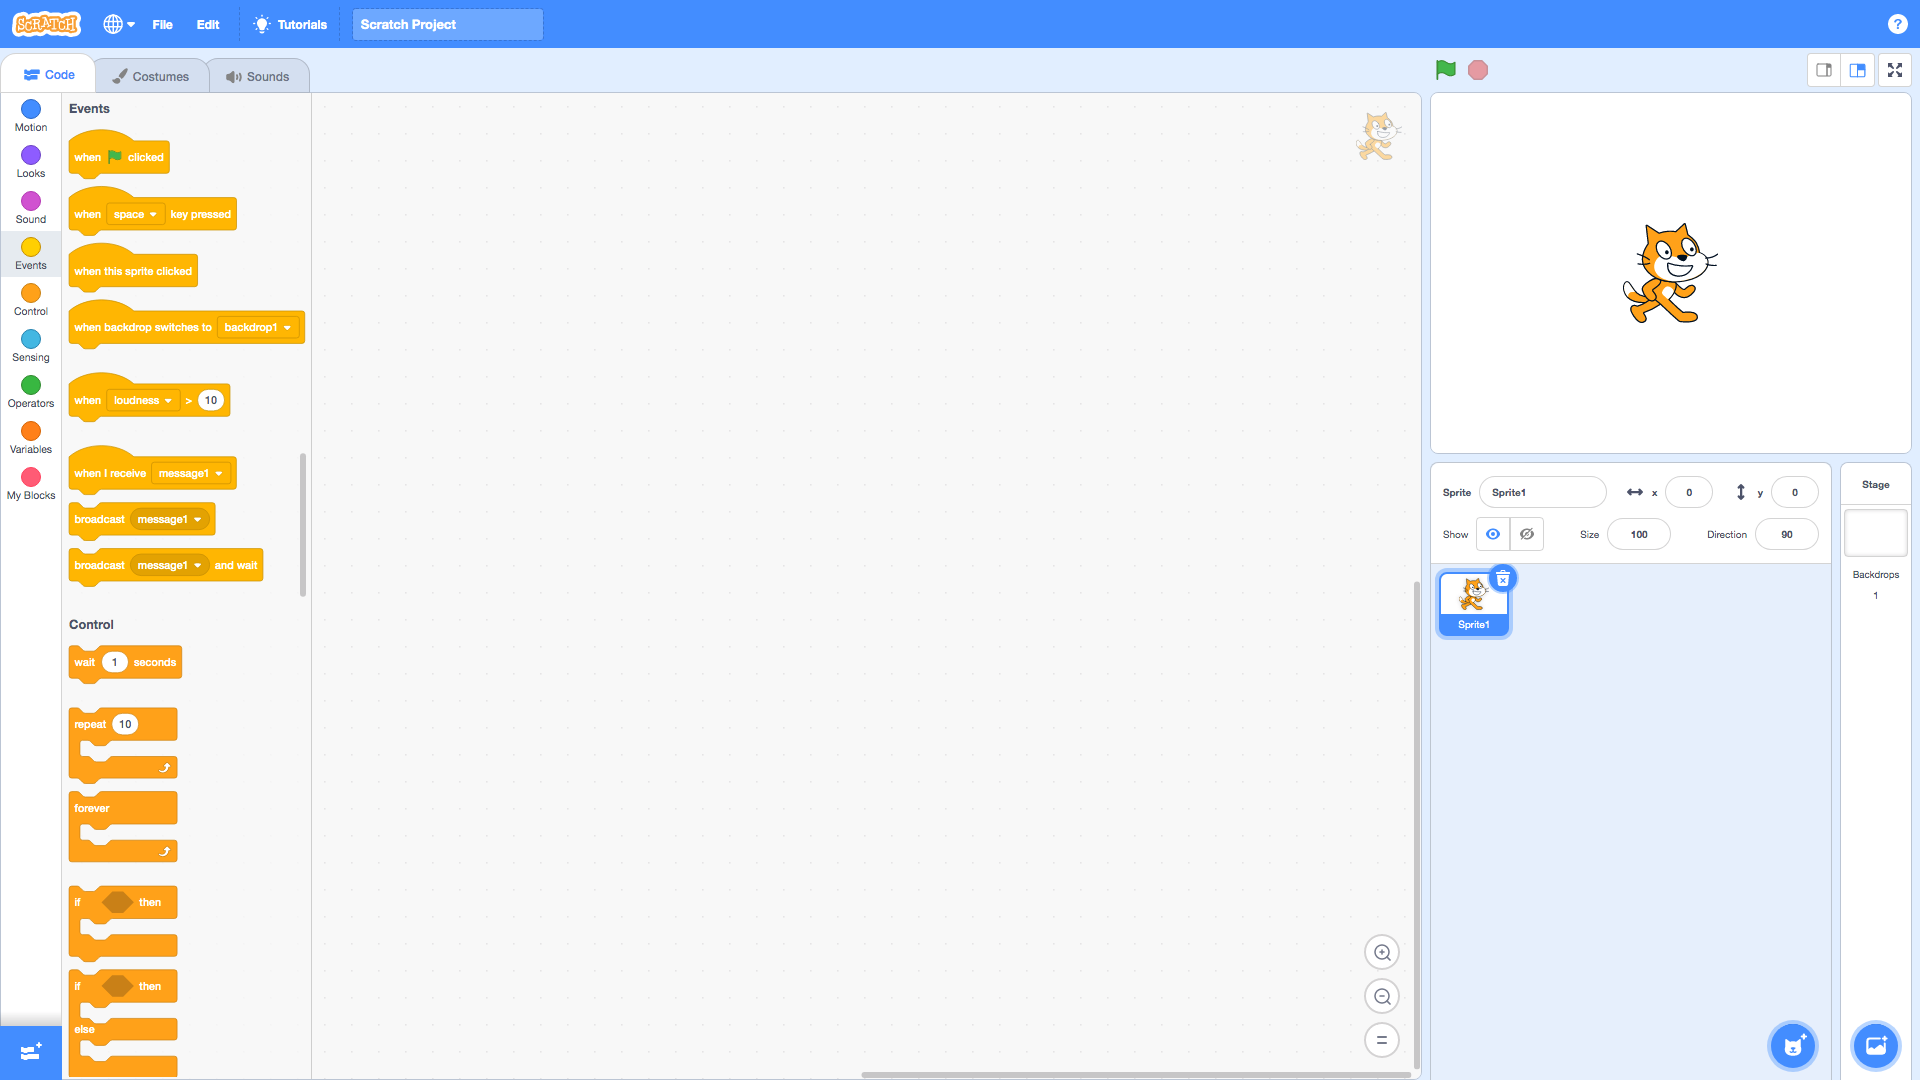
\includegraphics[width=1.0\linewidth,height=0.5\linewidth]{fig0051.png}
%  \caption{Групиране на инструкциите}
%\label{fig0051}
%\end{figure}
%
%Най-важното блокче в програмата е блокчето, което дава старт за изпълнение на инструкциите, които са подредени под него. Това блокче има зелен флаг (Фиг. \ref{fig0052}) и определя какво ще последва след стартирането на програмата.
%
%\begin{figure}[H]
%  \centering
%  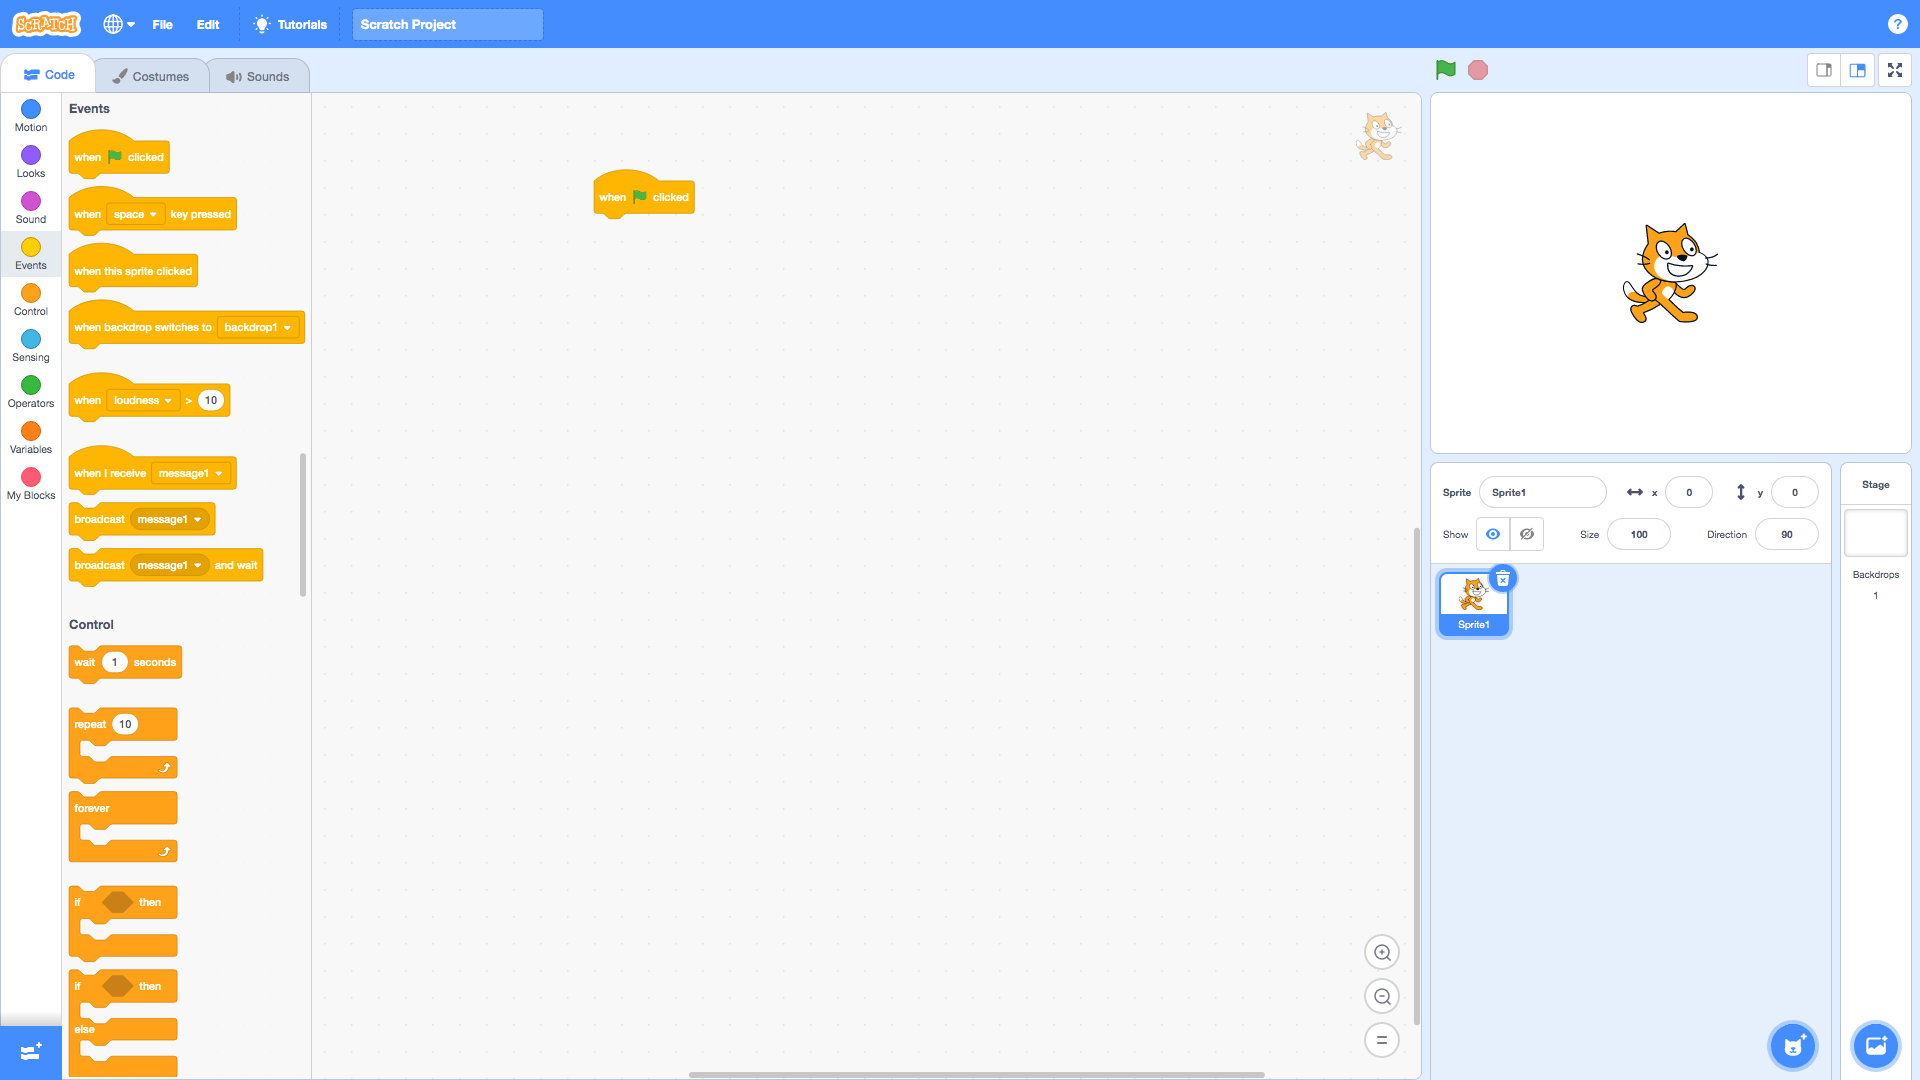
\includegraphics[width=1.0\linewidth,height=0.5\linewidth]{fig0052.png}
%  \caption{Начална точка на програмата}
%\label{fig0052}
%\end{figure}
%
%Блокчето за старт на програмата се намира в светло оранжевата група, която е предназначена да реагира на събития от страна на потребителя. Точният момент в който потребителят иска програмата да започне своето изпълнение е неопределен във времето и поради тази причина Scratch трябва да улови събитие, предизвикано от самия потребител. 
%
%Второто по важност блокче служи за край на програмата (Фиг. \ref{fig0053}). То се намира в тъмно оранжевата група и има за задача да спре всички процеси, извършващи се по време на изпълнението на самата програма.
%
%\begin{figure}[H]
%  \centering
%  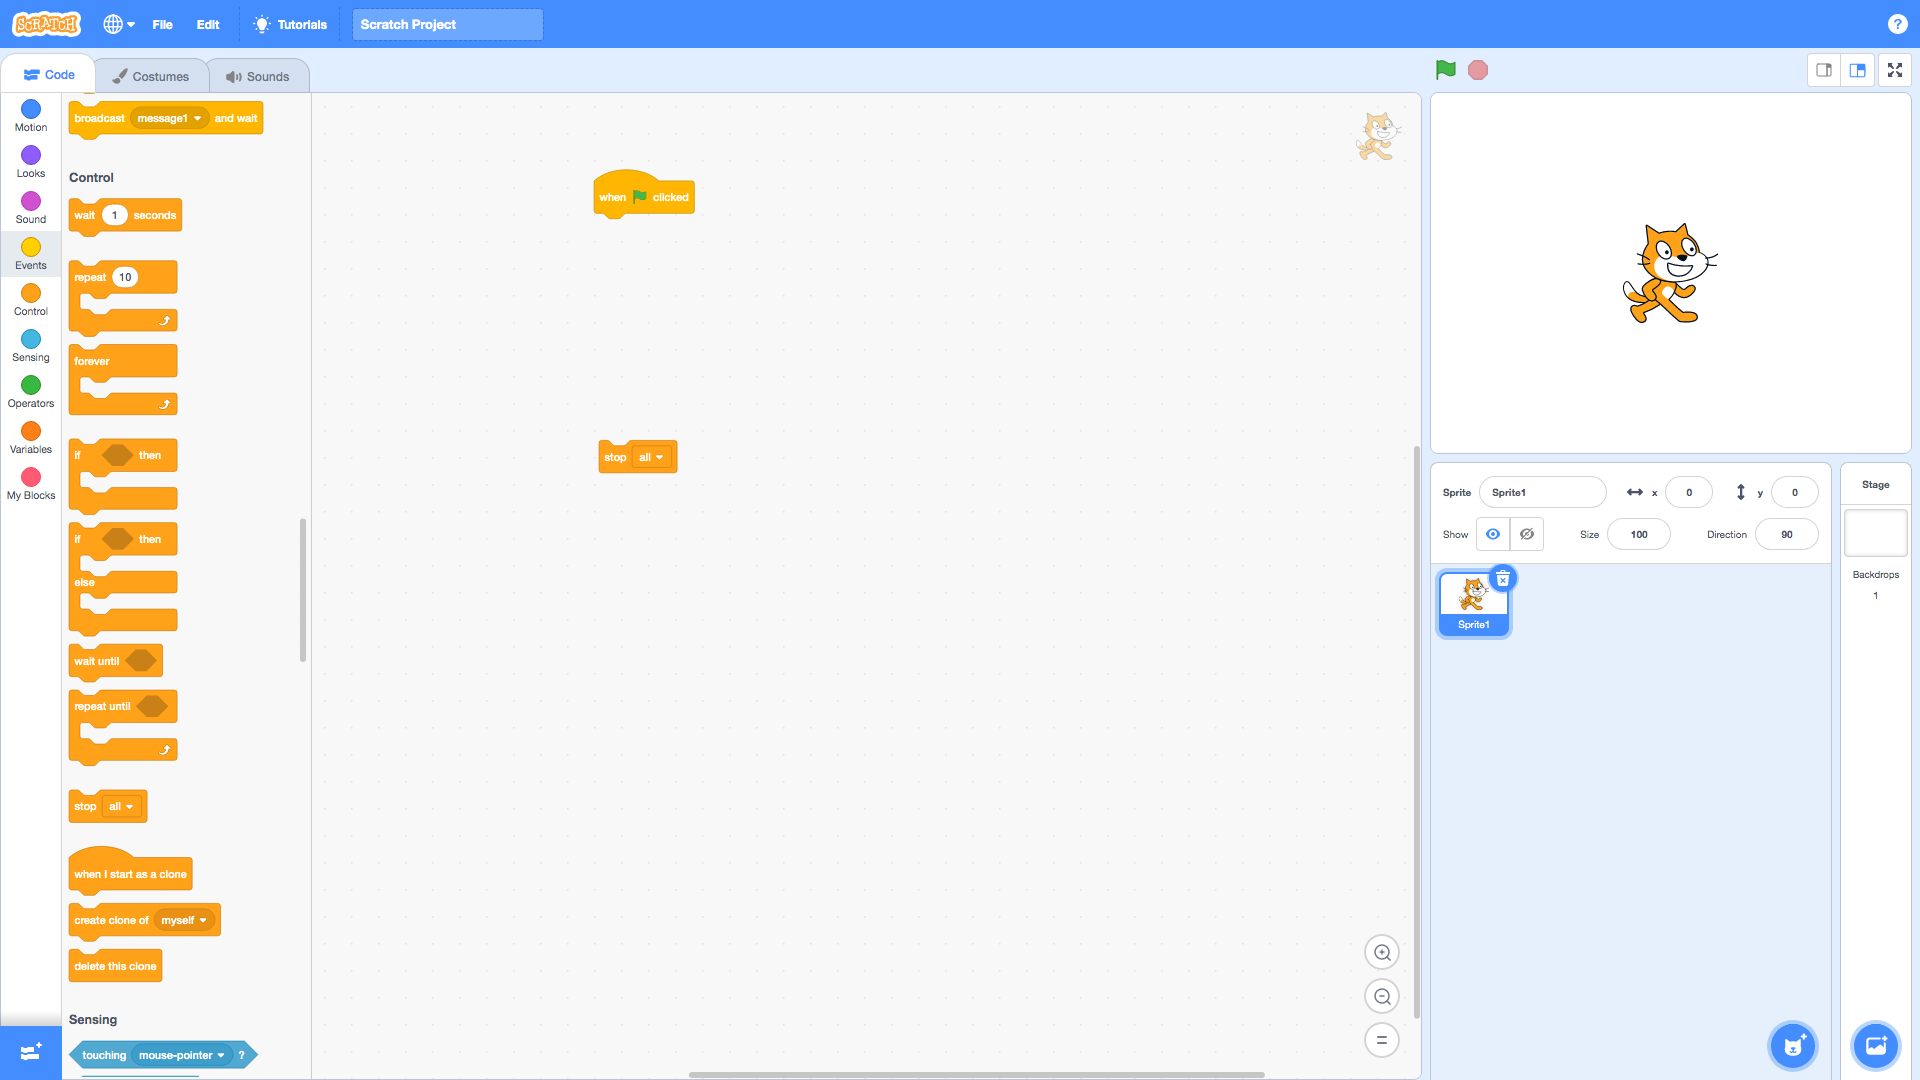
\includegraphics[width=1.0\linewidth,height=0.5\linewidth]{fig0053.png}
%  \caption{Крайна точка на програмата}
%\label{fig0053}
%\end{figure}
%
%Тъмно оранжевата група съдържа блокчета за контрол на изпълнението. Тези блокчета позволяват програмата да поема по различни пътища, както и група от действия да се повтарят многократно. 
%
%В Scratch блокчетата инструкции основно контролират картинки, наречени спрайтове (sprites). За разлика от обикновеното компютърно изображение, спрайтът е графичен обект, който съдържа множество кадри, показващи изображението на героя в различни конфигурации. Всяка нова програма в Scratch започва с един спрайт, на оранжевата котка, разположена на координати (x=0,y=0). Работното пространство е двуизмерна координатна система с център (0,0). 
%
%\begin{figure}[H]
%  \centering
%  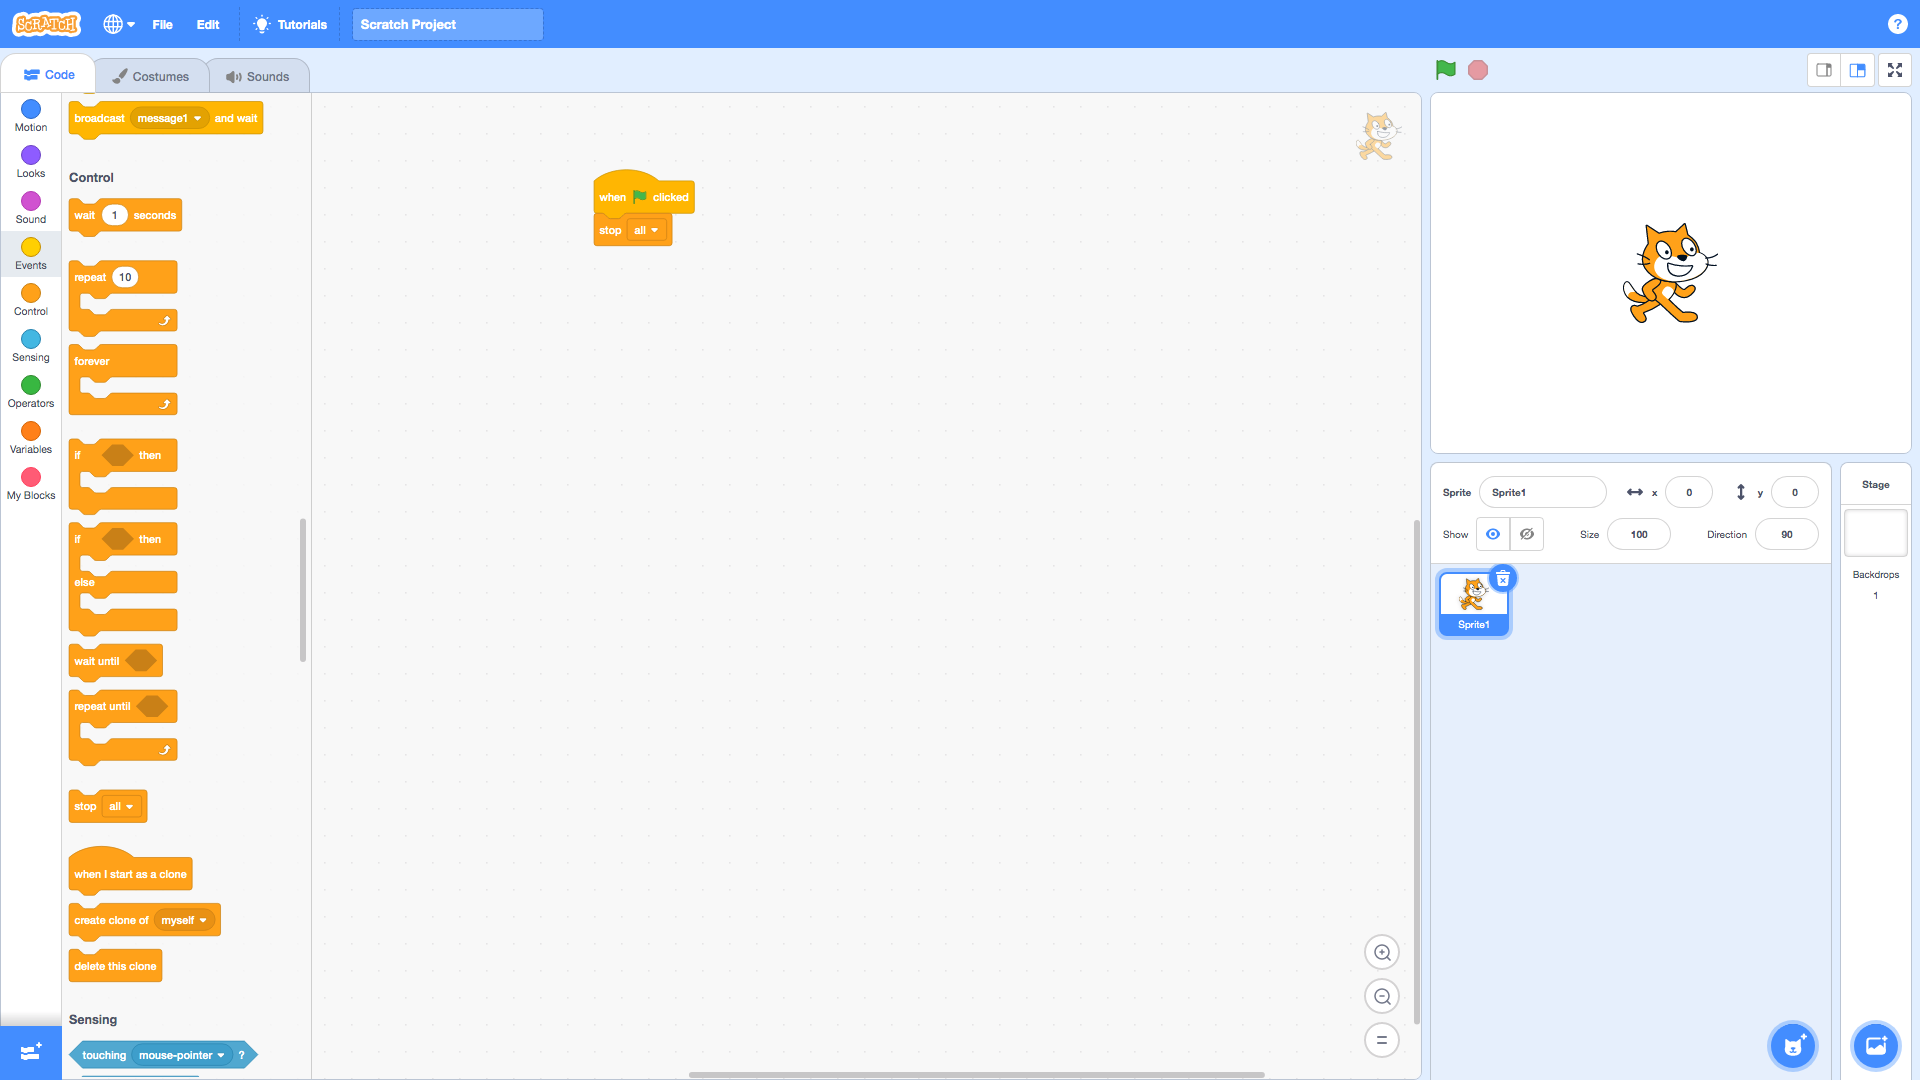
\includegraphics[width=1.0\linewidth,height=0.5\linewidth]{fig0054.png}
%  \caption{Завършване веднага след започване}
%\label{fig0054}
%\end{figure}
%
%Ако бъдат съединени, блокчетата за начало и за край (Фиг. \ref{fig0054}), то програмата не изпълнява нищо. Практически, тази програма приключва веднага след като е започнала. Програма, която не прави нищо е напълно безсмислена. За да започне нещо да се случва се използват блокчетата в синята група. Първото блокче инструктира котето да се премести 10 стъпки, като броя стъпки може да бъде променени, чрез изписване на друго число във вътрешността на блокчето (Фиг. \ref{fig0055}).
%
%\begin{figure}[H]
%  \centering
%  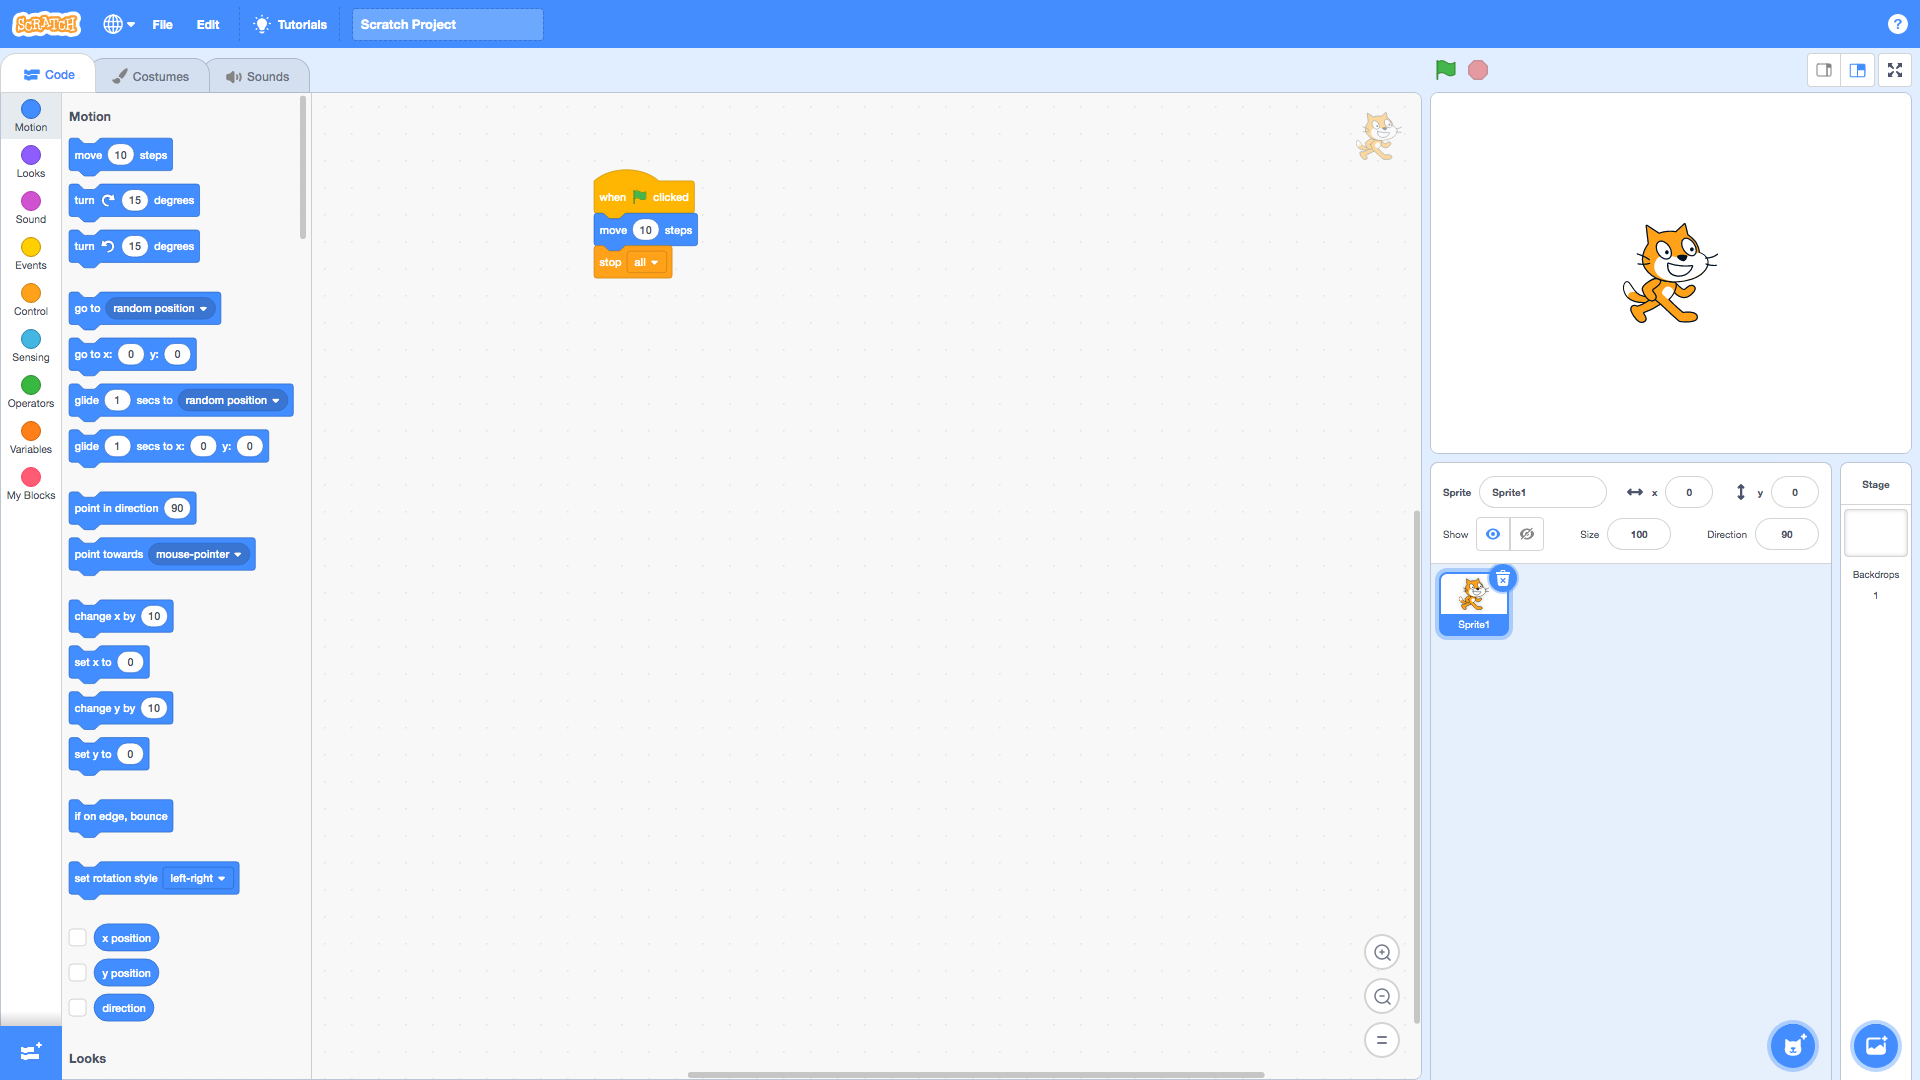
\includegraphics[width=1.0\linewidth,height=0.5\linewidth]{fig0055.png}
%  \caption{Преместване на героя}
%\label{fig0055}
%\end{figure}
%
%Следващият блок в групата инструктира героя да се завърти на определено число градуси, по часовниковата стрелка, спрямо собствения си център (Фиг. \ref{fig0056}).
%
%\begin{figure}[H]
%  \centering
%  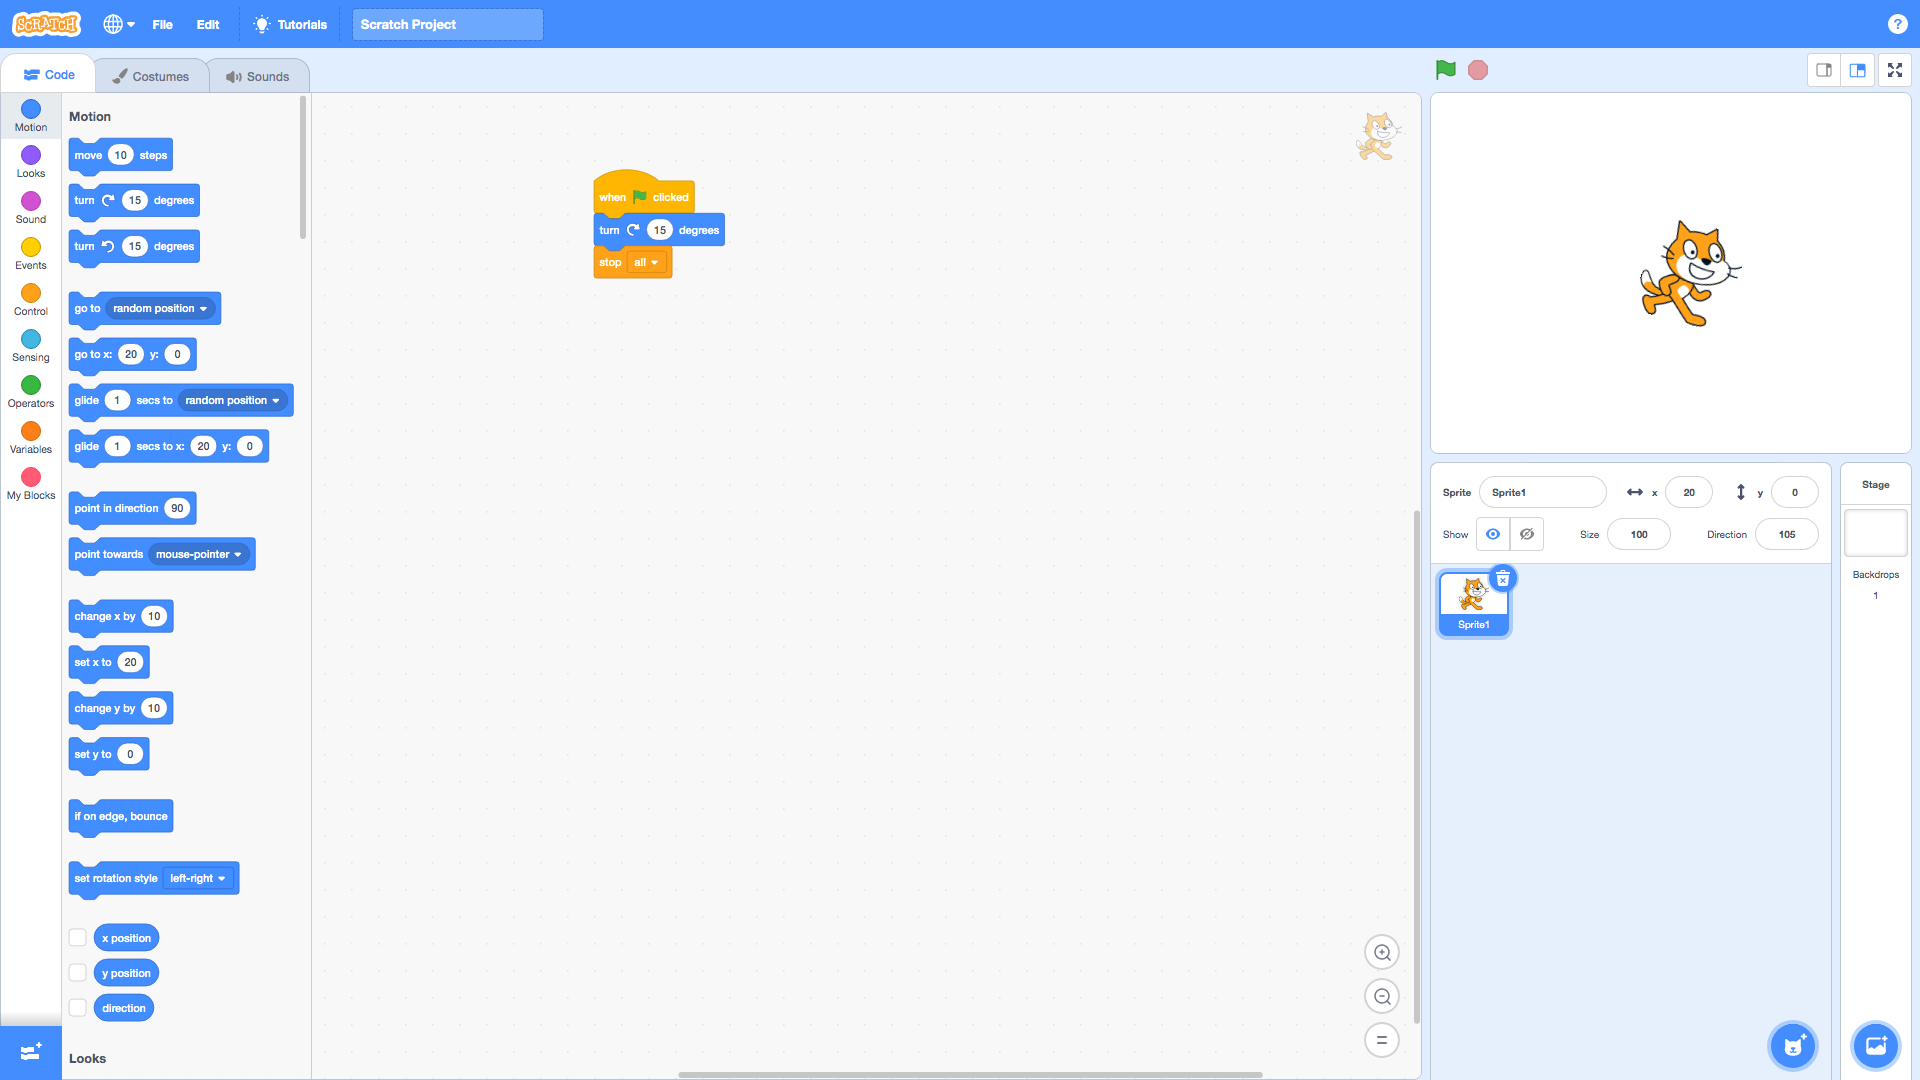
\includegraphics[width=1.0\linewidth,height=0.5\linewidth]{fig0056.png}
%  \caption{Завъртане по часовниковата стрелка}
%\label{fig0056}
%\end{figure}
%
%Аналогично, със следващото блокче в групата, завъртането може да се изпълни и в посока обратна на часовниковата стрелка (Фиг. \ref{fig0057}).
%
%\begin{figure}[H]
%  \centering
%  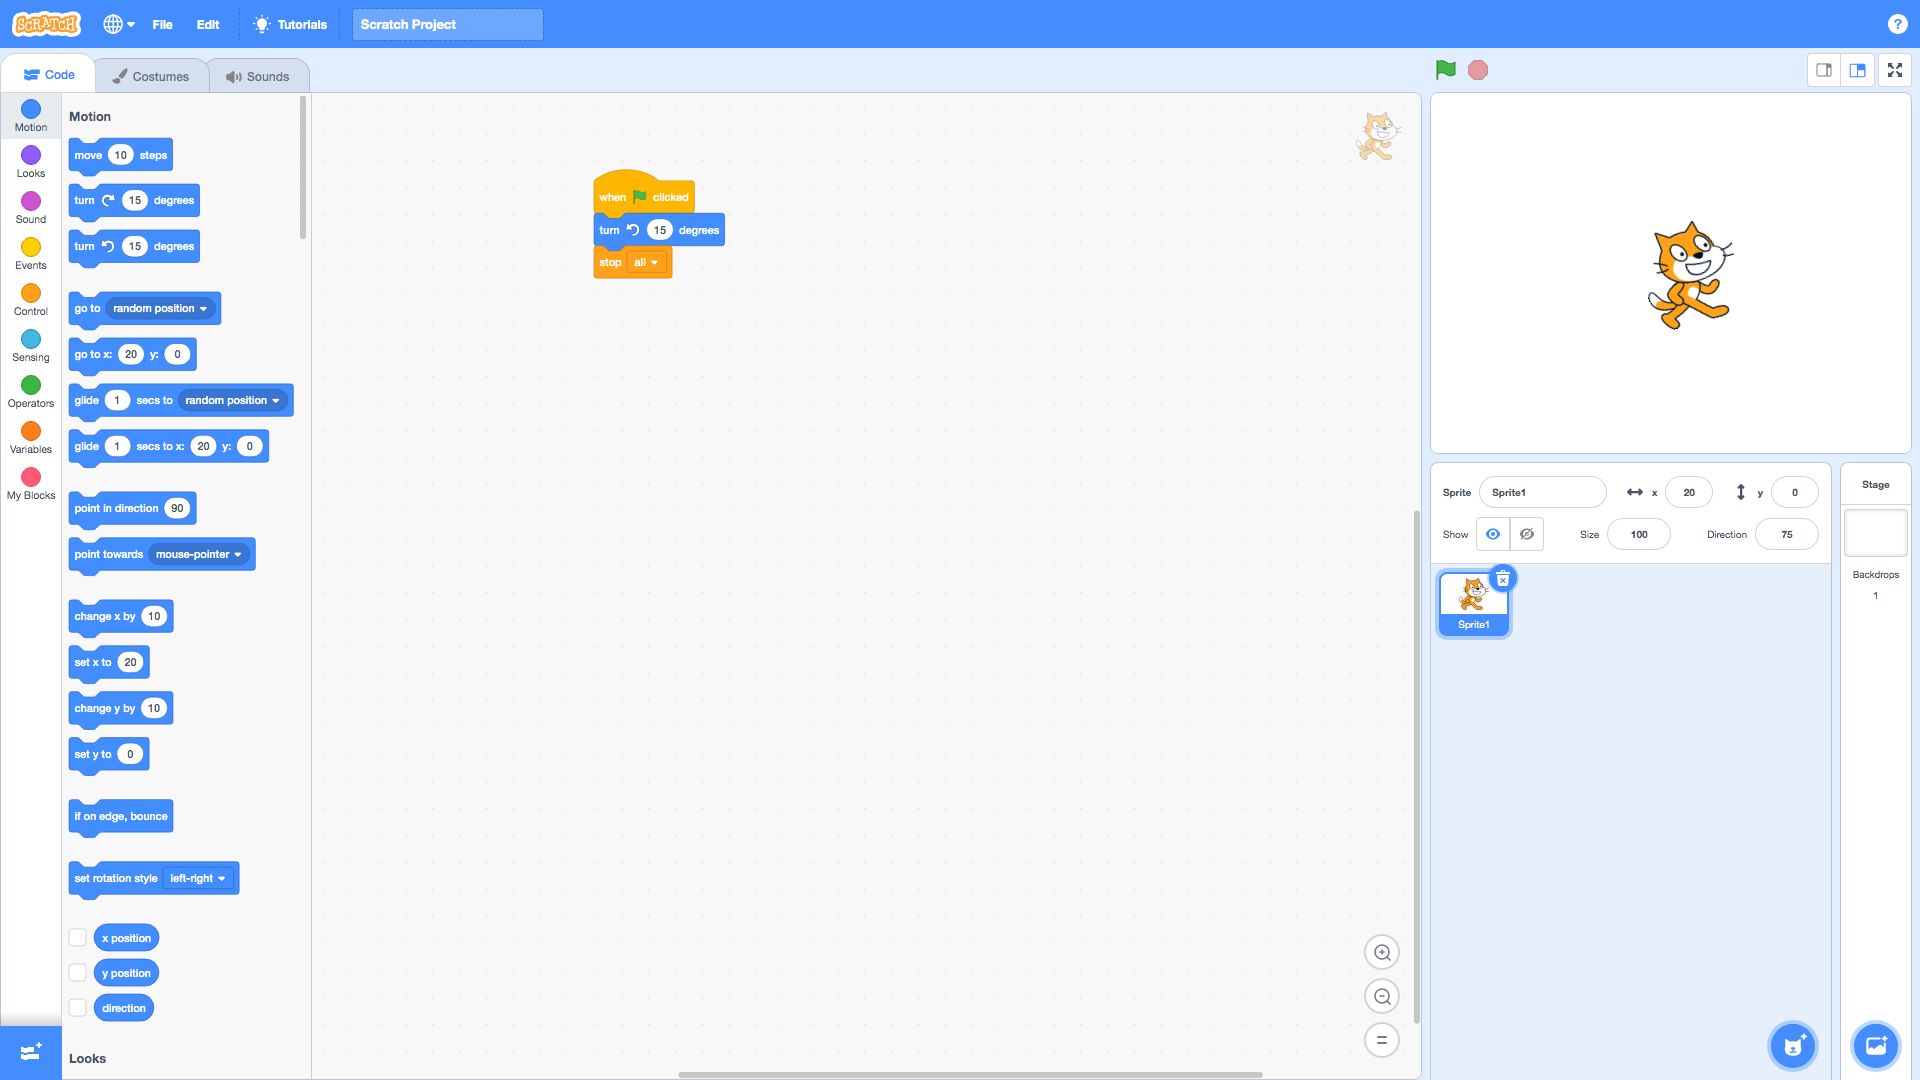
\includegraphics[width=1.0\linewidth,height=0.5\linewidth]{fig0057.png}
%  \caption{Завъртане обратно на часовниковата стрелка}
%\label{fig0057}
%\end{figure}
%
%Следващия блок в групата дава възможност героят да се премести на случайни координати или на координати посочени с мишката (Фиг. \ref{fig0058}).
%
%\begin{figure}[H]
%  \centering
%  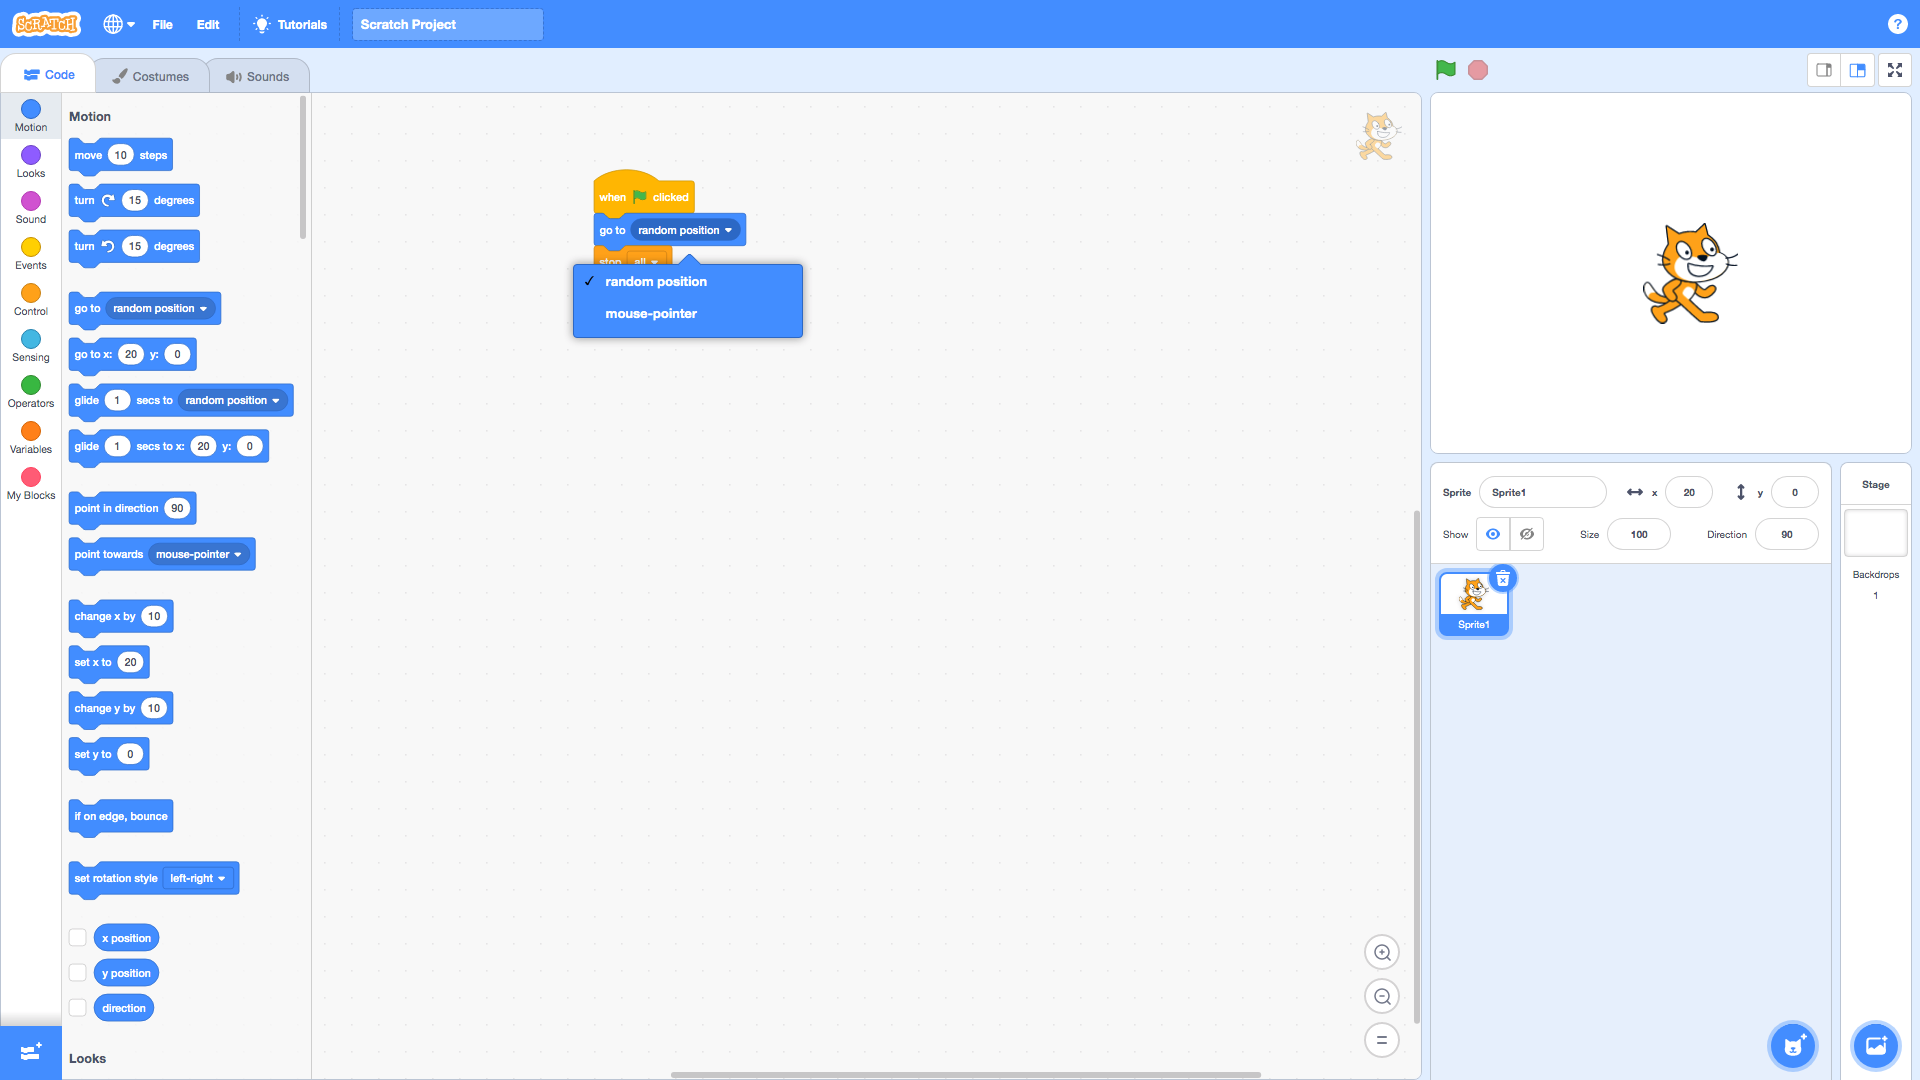
\includegraphics[width=1.0\linewidth,height=0.5\linewidth]{fig0058.png}
%  \caption{Преместване на случайна позиция}
%\label{fig0058}
%\end{figure}
%
%Движението на героя може да бъде зададено и чрез абсолютни координати с блокче, позволяващо да се впишат числа за абцисната и ординатната ос (Фиг. \ref{fig0059}).
%
%\begin{figure}[H]
%  \centering
%  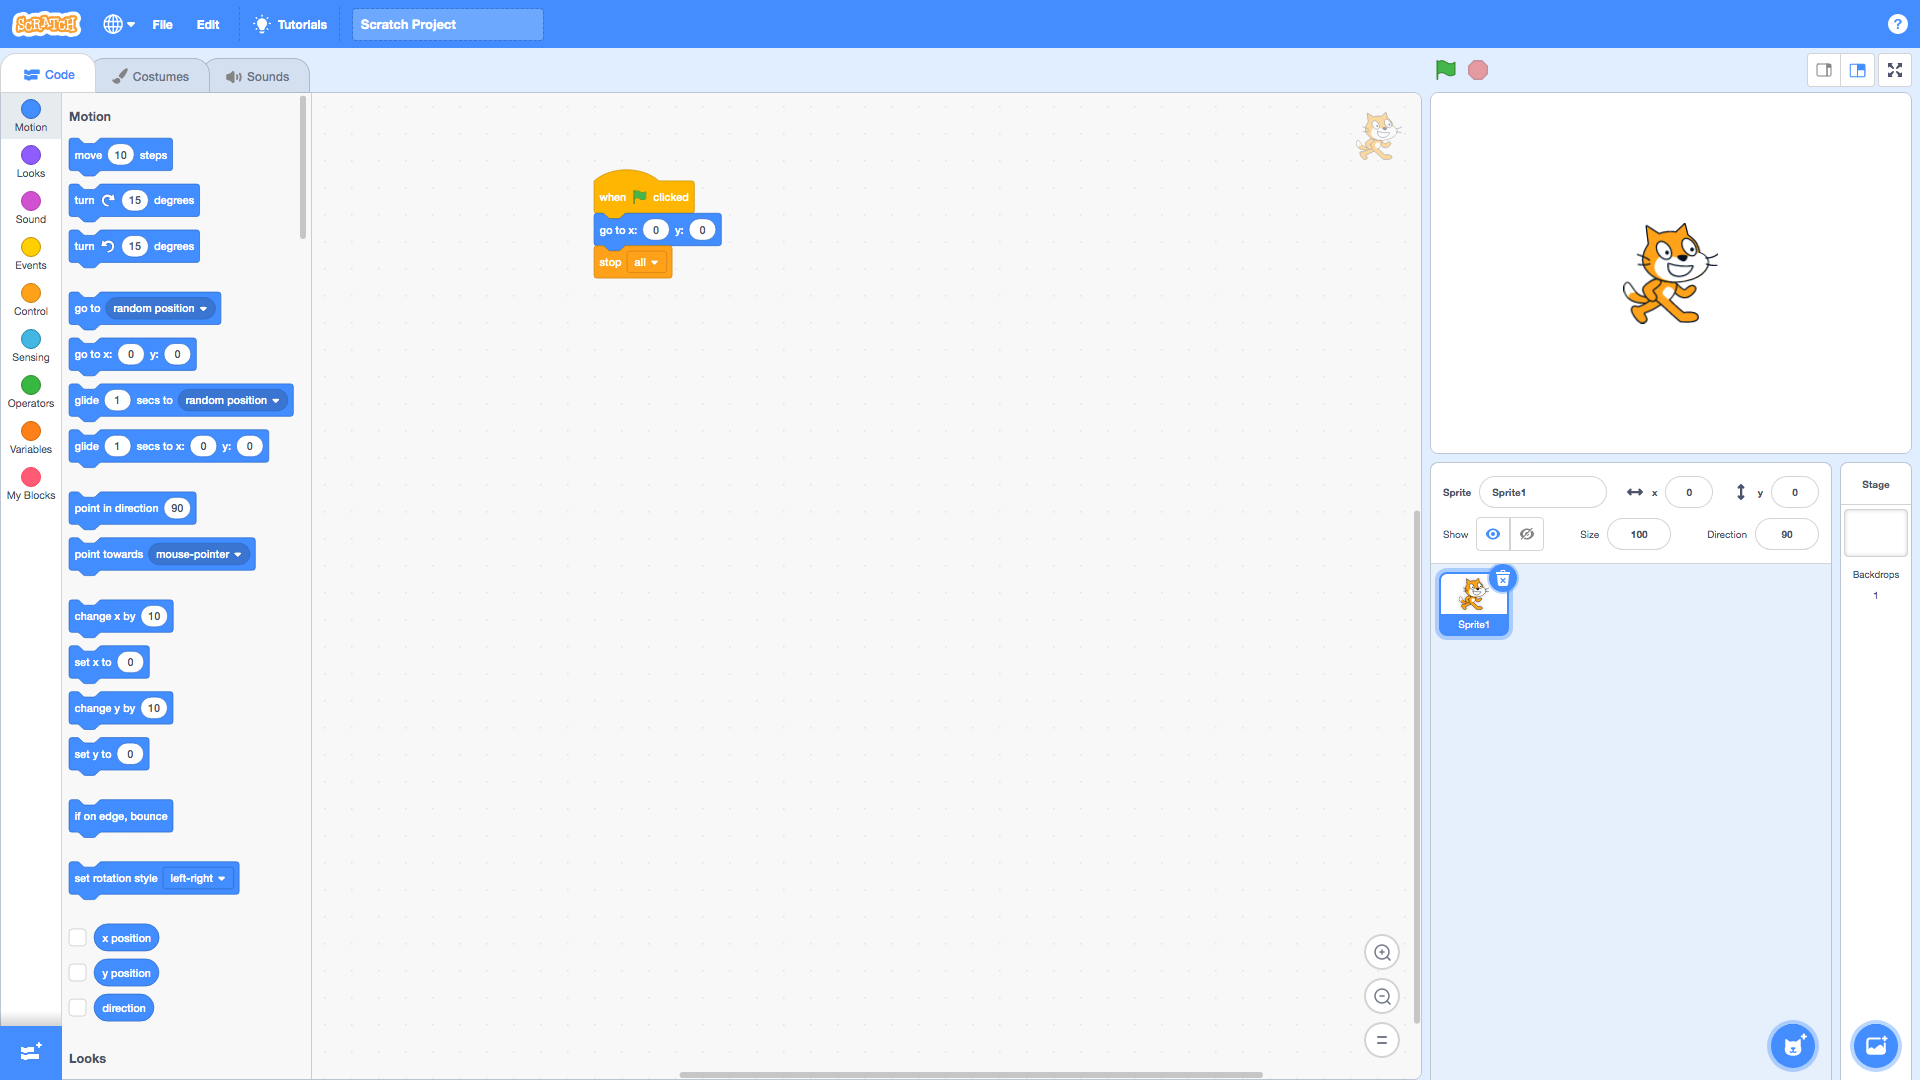
\includegraphics[width=1.0\linewidth,height=0.5\linewidth]{fig0059.png}
%  \caption{Преместване по абсолютни координати}
%\label{fig0059}
%\end{figure}
%
%Плавно придвижване, по предварително зададен интервал от време, е възможно на случайни координати или координати посочени с мишката, благодарение на следващото блокче в групата (Фиг. \ref{fig0060}).
%
%\begin{figure}[H]
%  \centering
%  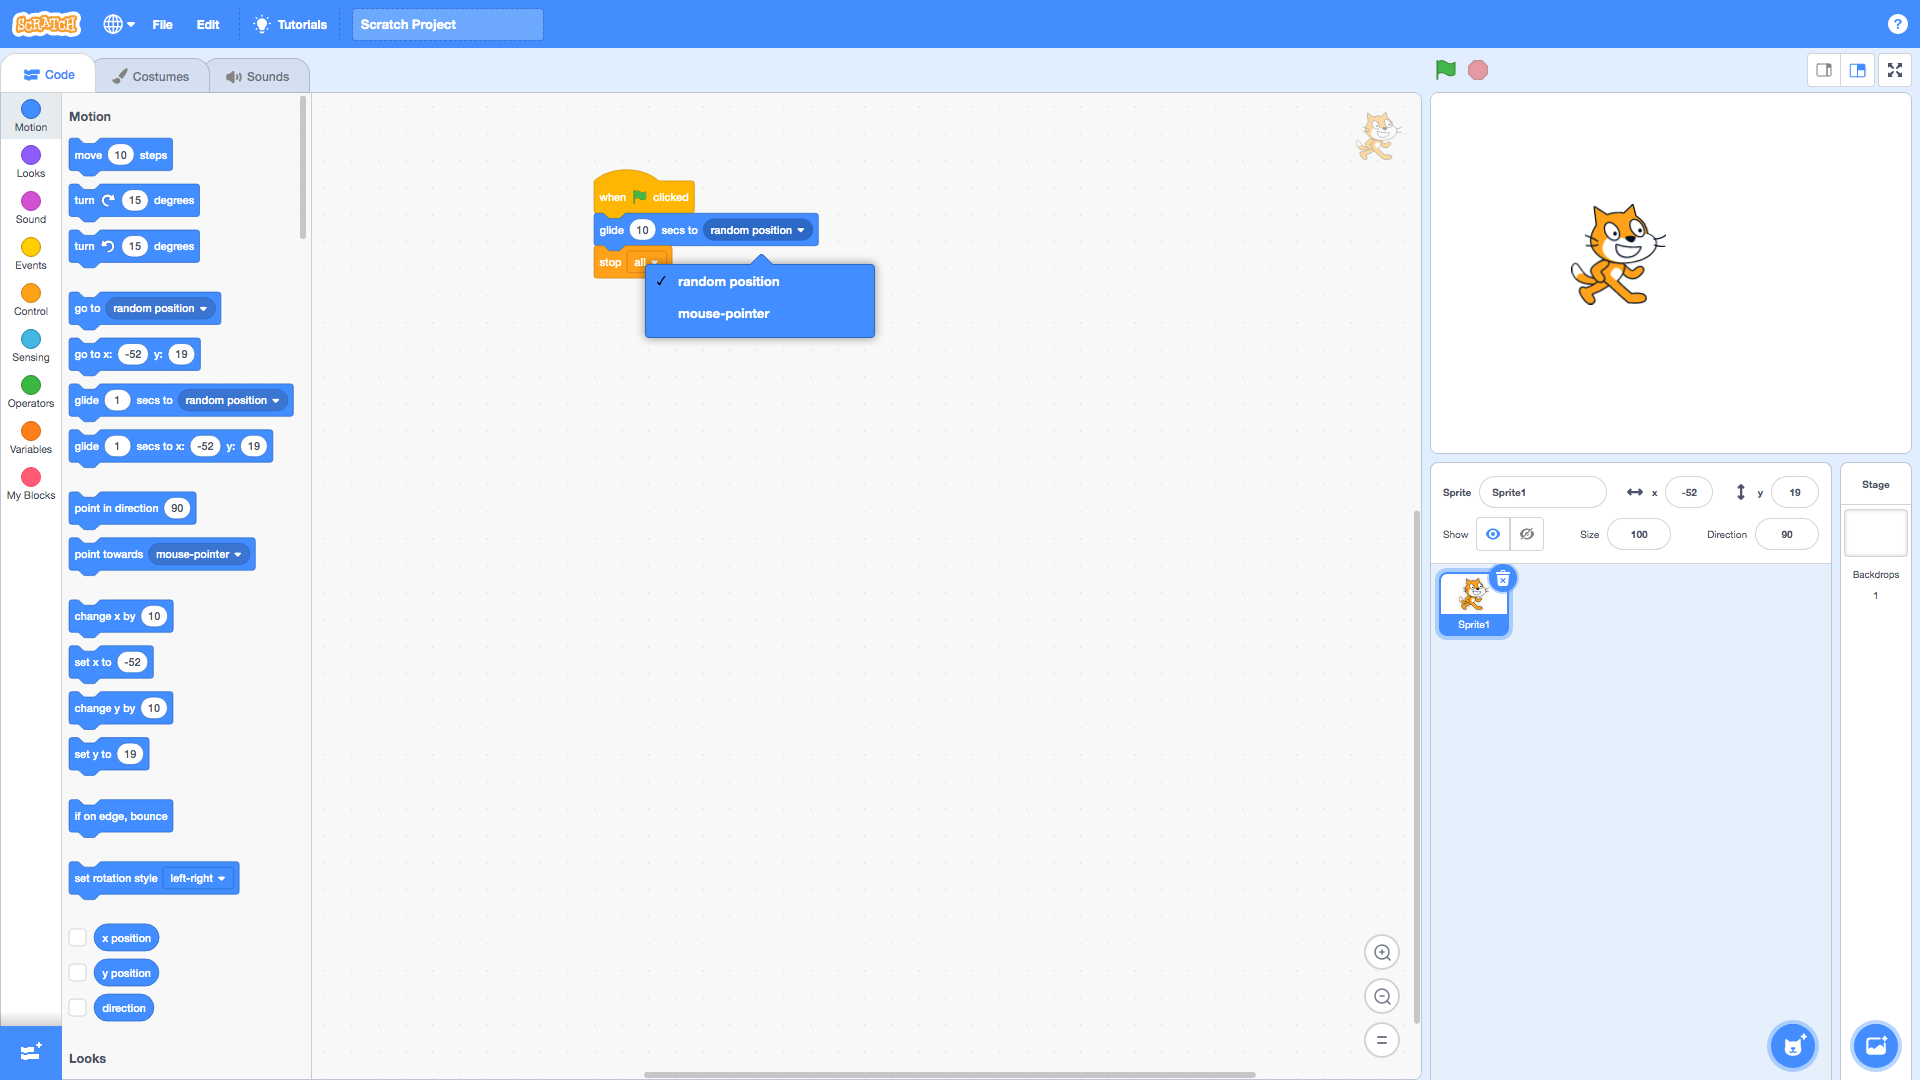
\includegraphics[width=1.0\linewidth,height=0.5\linewidth]{fig0060.png}
%  \caption{Плъзгане до случайна позиция}
%\label{fig0060}
%\end{figure}
%
%Плавното плъзгане до предварително зададени координати, за предварително определен интервал от време, е възможно с блокчето предназначено за тази цел (Фиг. \ref{fig0061}).
%
%\begin{figure}[H]
%  \centering
%  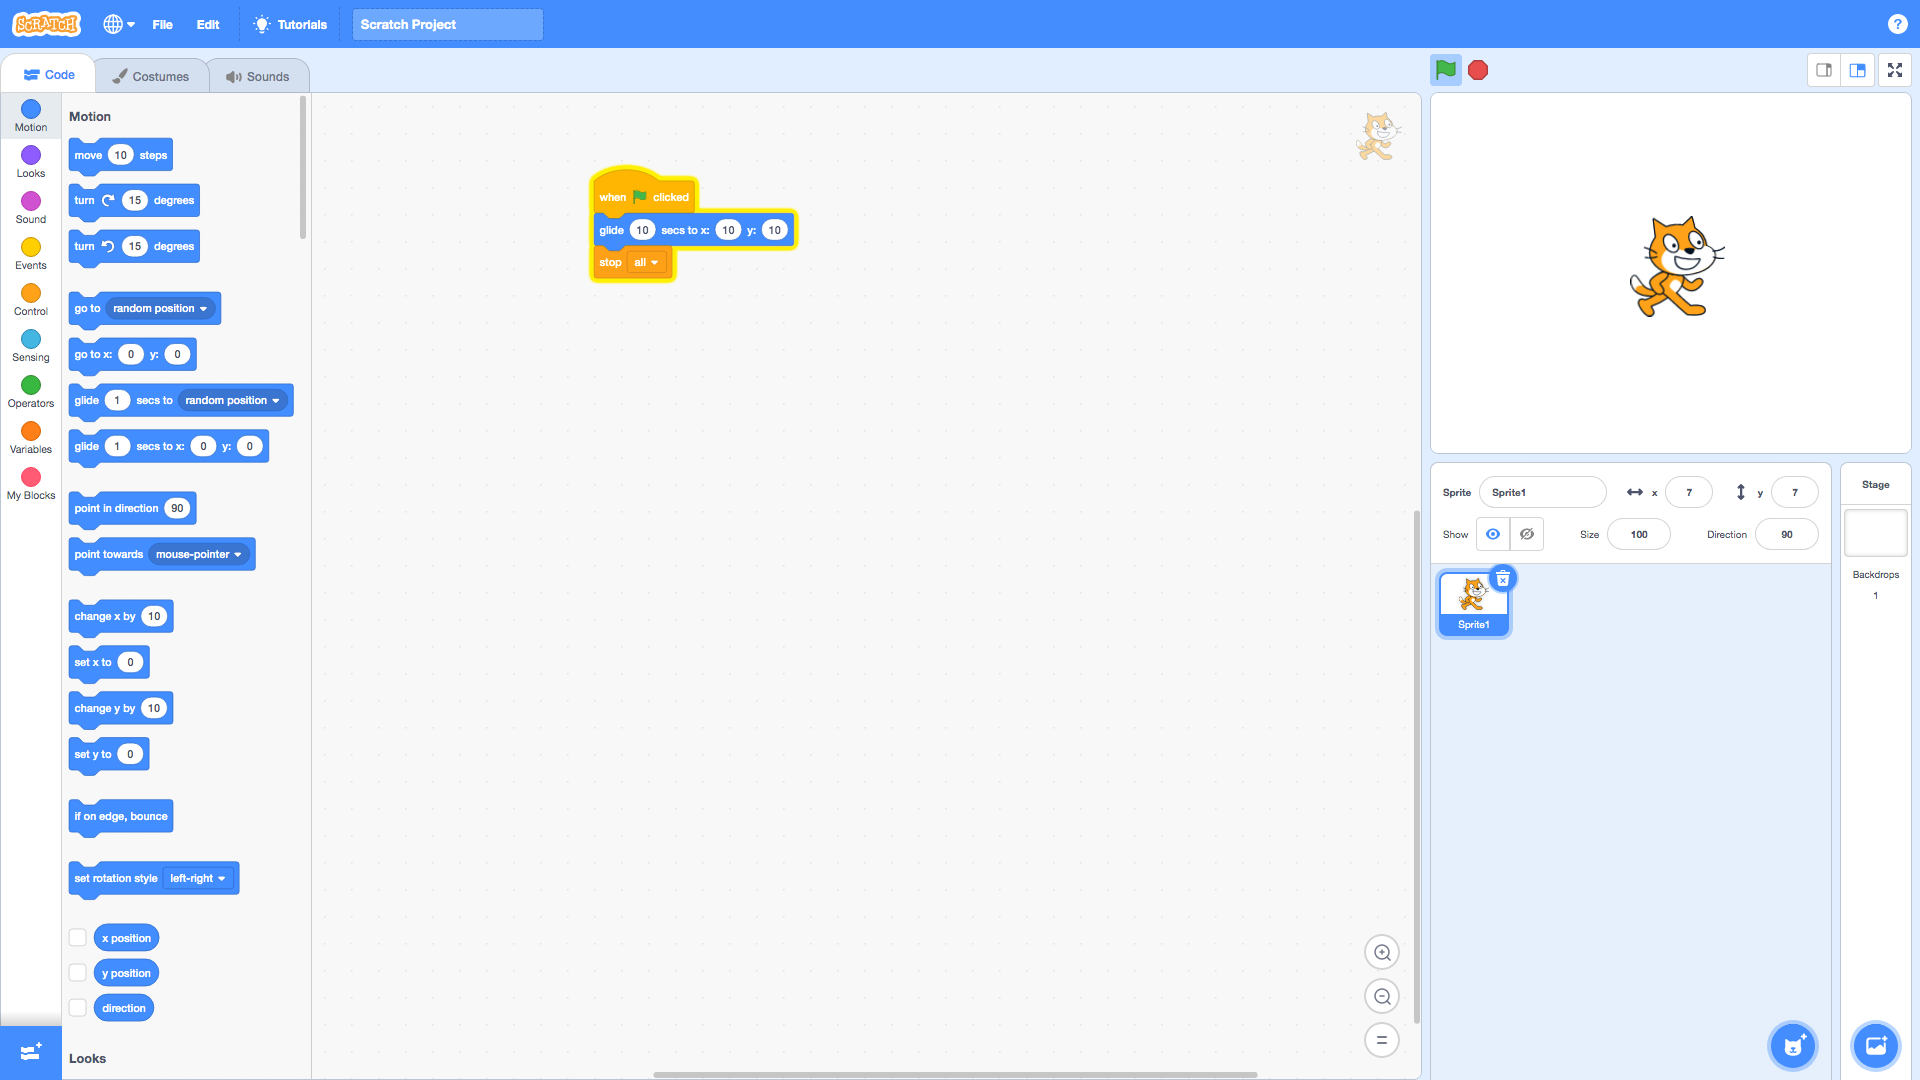
\includegraphics[width=1.0\linewidth,height=0.5\linewidth]{fig0061.png}
%  \caption{Плъзгане до зададени координати}
%\label{fig0061}
%\end{figure}
%
%Анимираният герой има характеристика за ориентация, под формата на ъгъл. При 90 градуса, оранжевата котка гледа на дясно. За да се промени ориентацията на героя се използва блокче с възможност за въвеждане на конкретен ъгъл (Фиг. \ref{fig0062}).
%
%\begin{figure}[H]
%  \centering
%  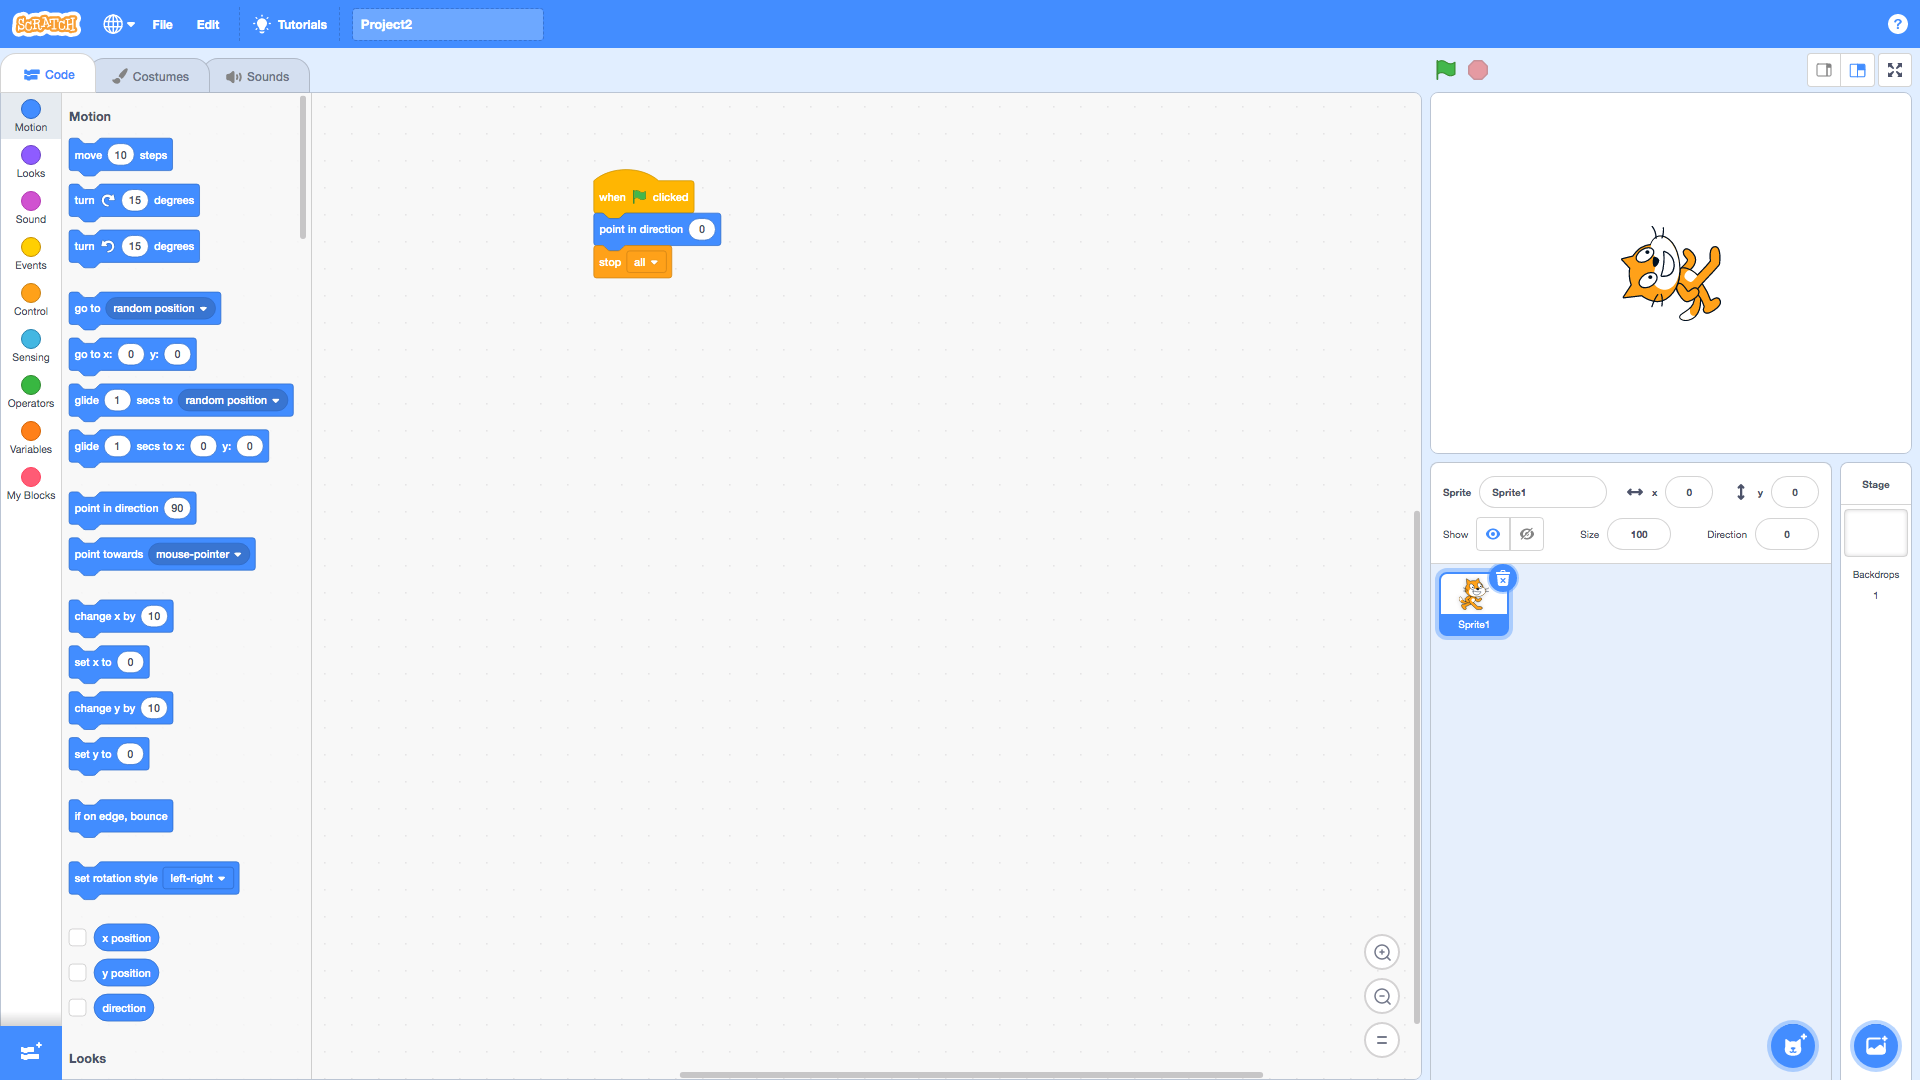
\includegraphics[width=1.0\linewidth,height=0.5\linewidth]{fig0062.png}
%  \caption{Ъглова ориентация}
%\label{fig0062}
%\end{figure}
%
%При по-сложни сценарии за управление на героя, понякога е нужно героят да следи показалеца на мишката. За тази цел има определено блокче, което изпълнява тази инструкция (Фиг. \ref{fig0063}).
%
%\begin{figure}[H]
%  \centering
%  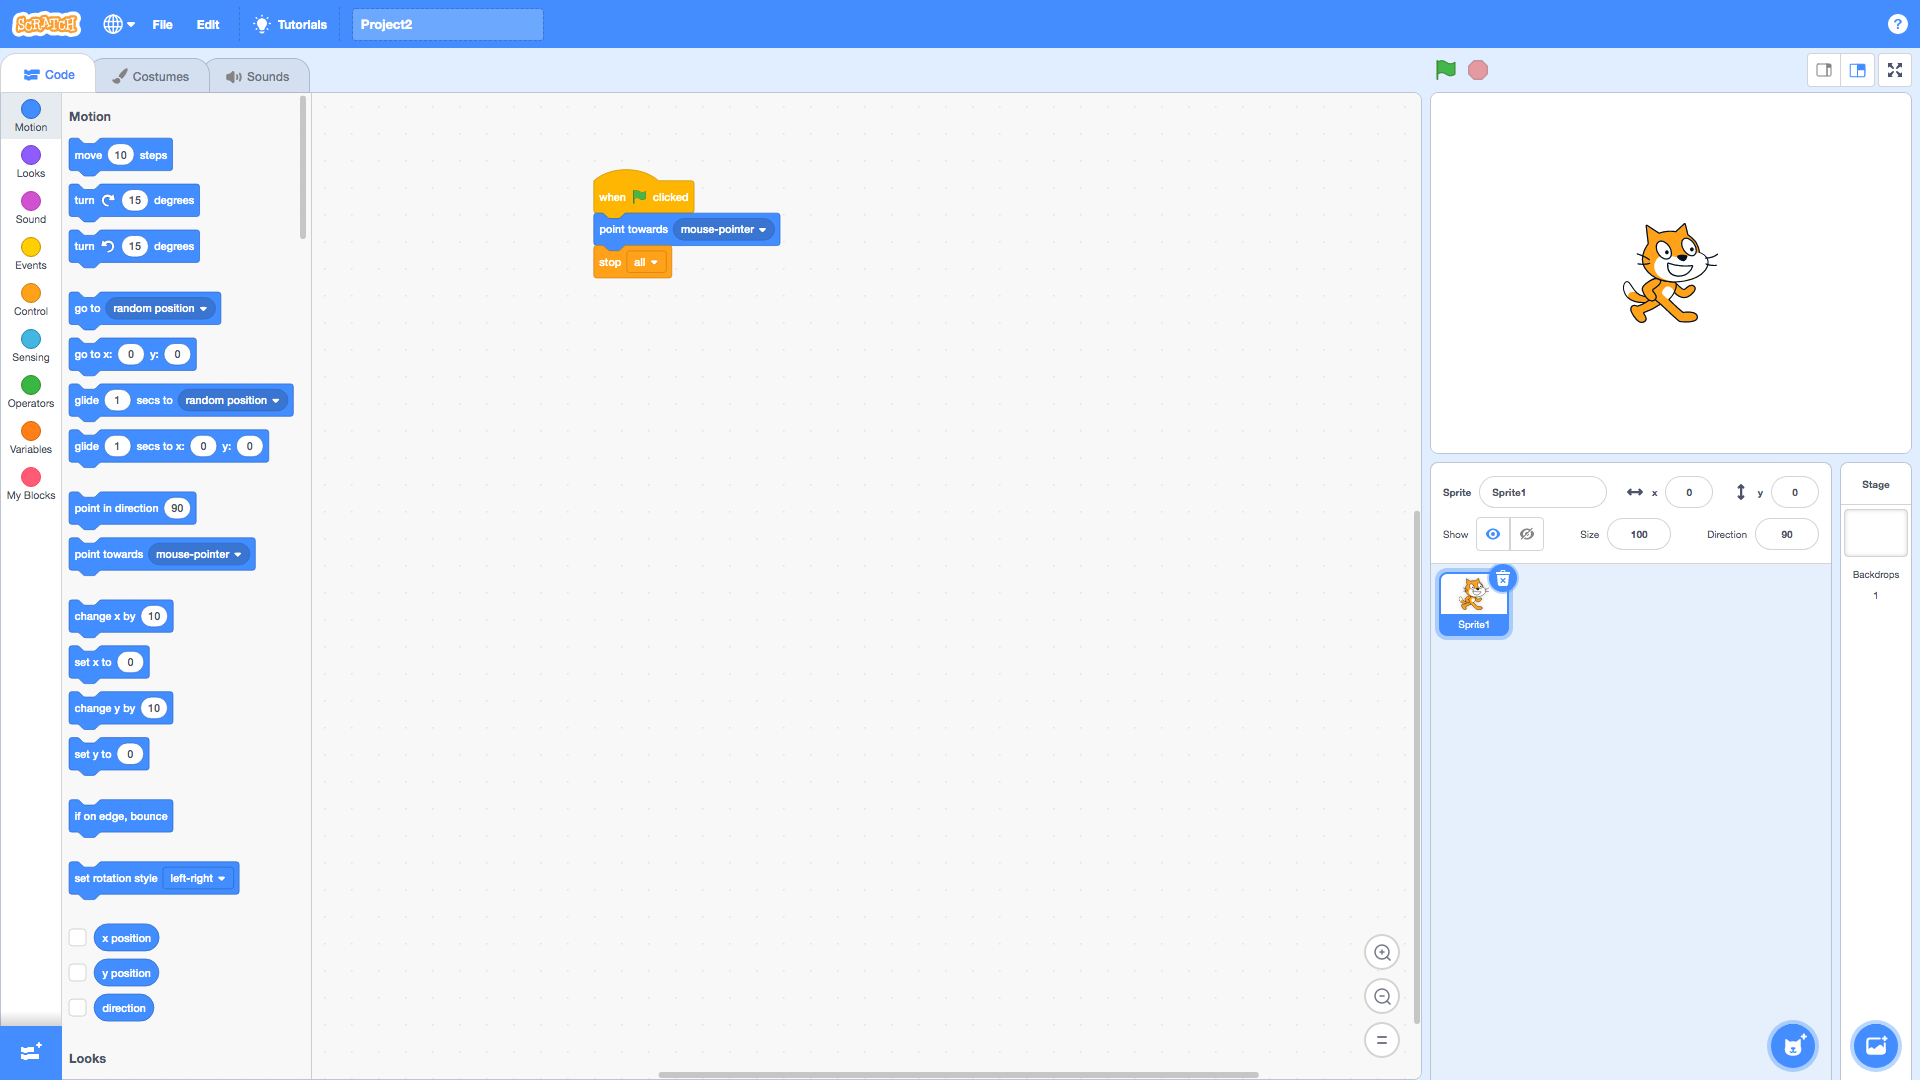
\includegraphics[width=1.0\linewidth,height=0.5\linewidth]{fig0063.png}
%  \caption{Ориентация по показалеца на мишката}
%\label{fig0063}
%\end{figure}
%
%Блокчетата могат да се поставят едно след друго, като за последователна промяна на относителните x и y координатите (относителни, спрямо текущата позиция) на героя има специално определени блокчета (Фиг. \ref{fig0064}).
%
%\begin{figure}[H]
%  \centering
%  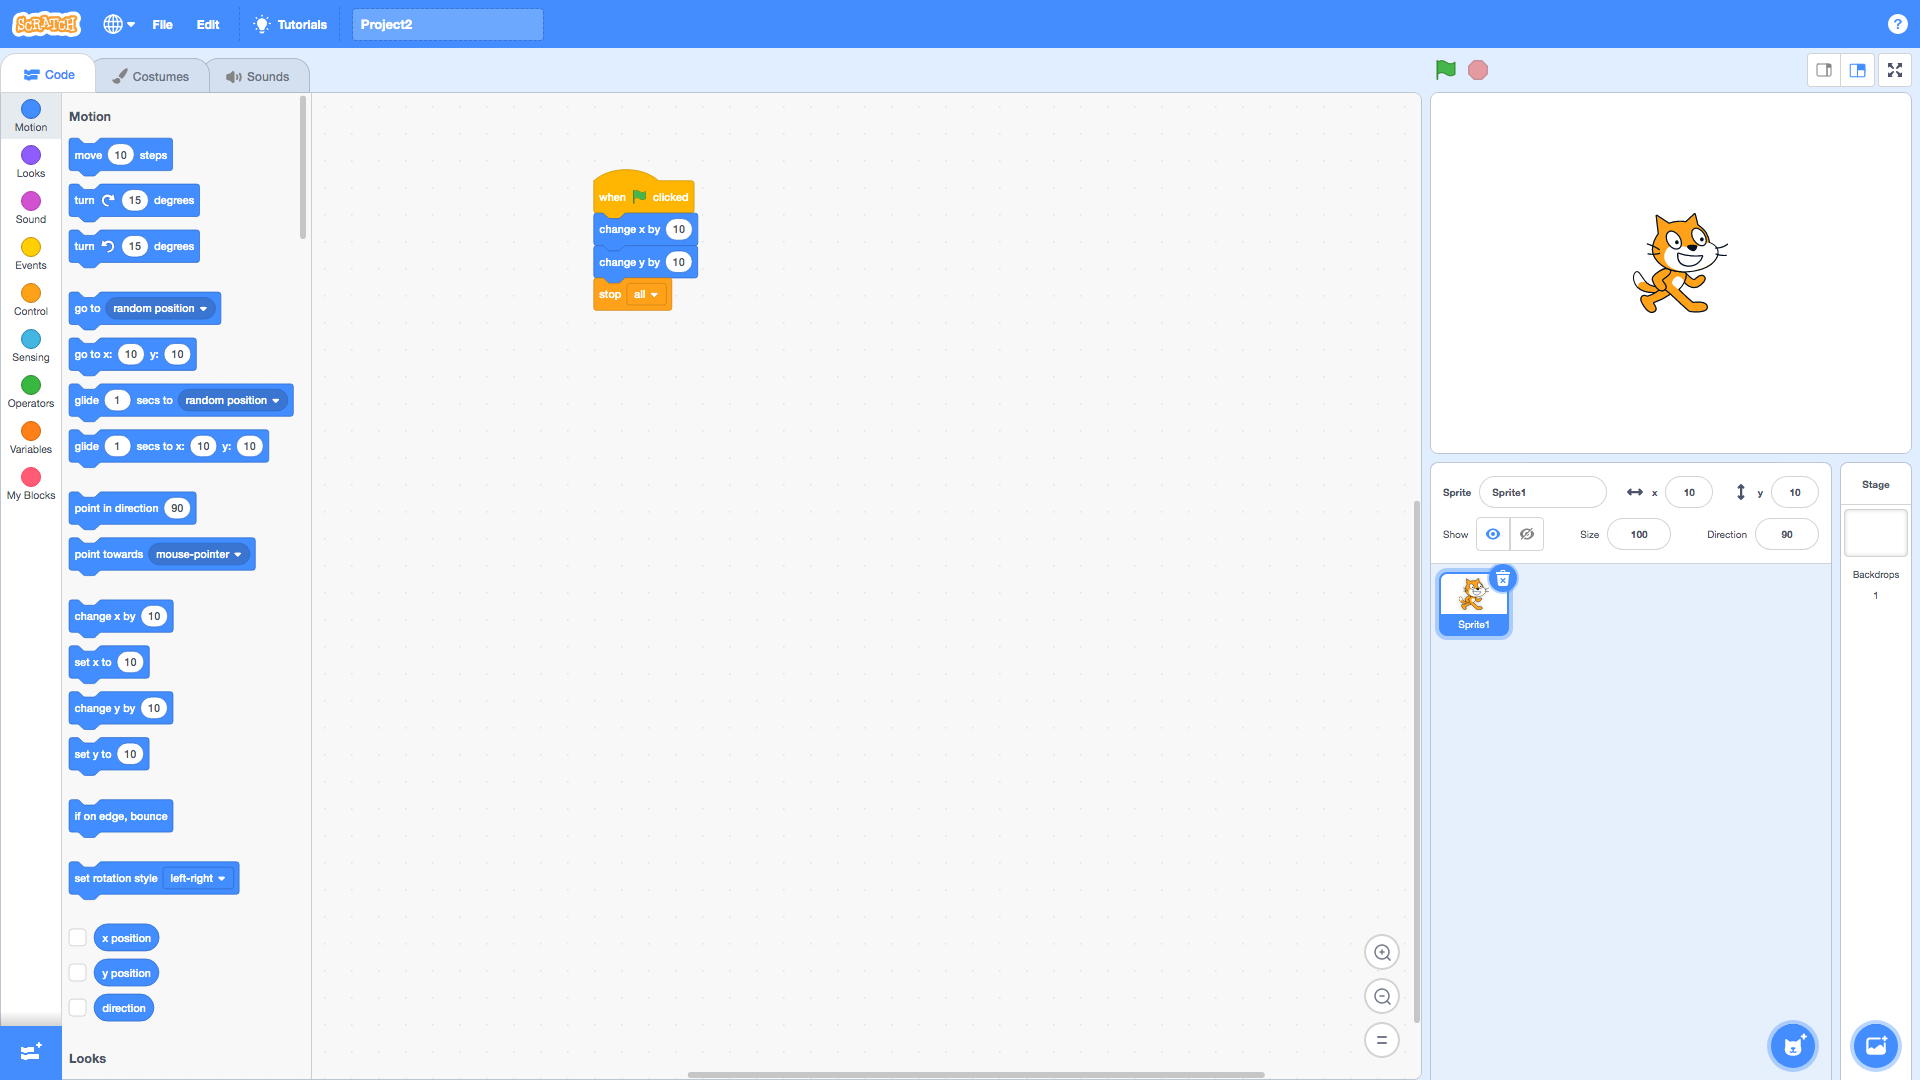
\includegraphics[width=1.0\linewidth,height=0.5\linewidth]{fig0064.png}
%  \caption{Последователна промяна на относителни координати}
%\label{fig0064}
%\end{figure}
%
%Освен относителна промяна на координатите е възможна и абсолютна промяна на координатите, като абсолютната промяна е спрямо центъра на координатната система (Фиг. \ref{fig0065}).
%
%\begin{figure}[H]
%  \centering
%  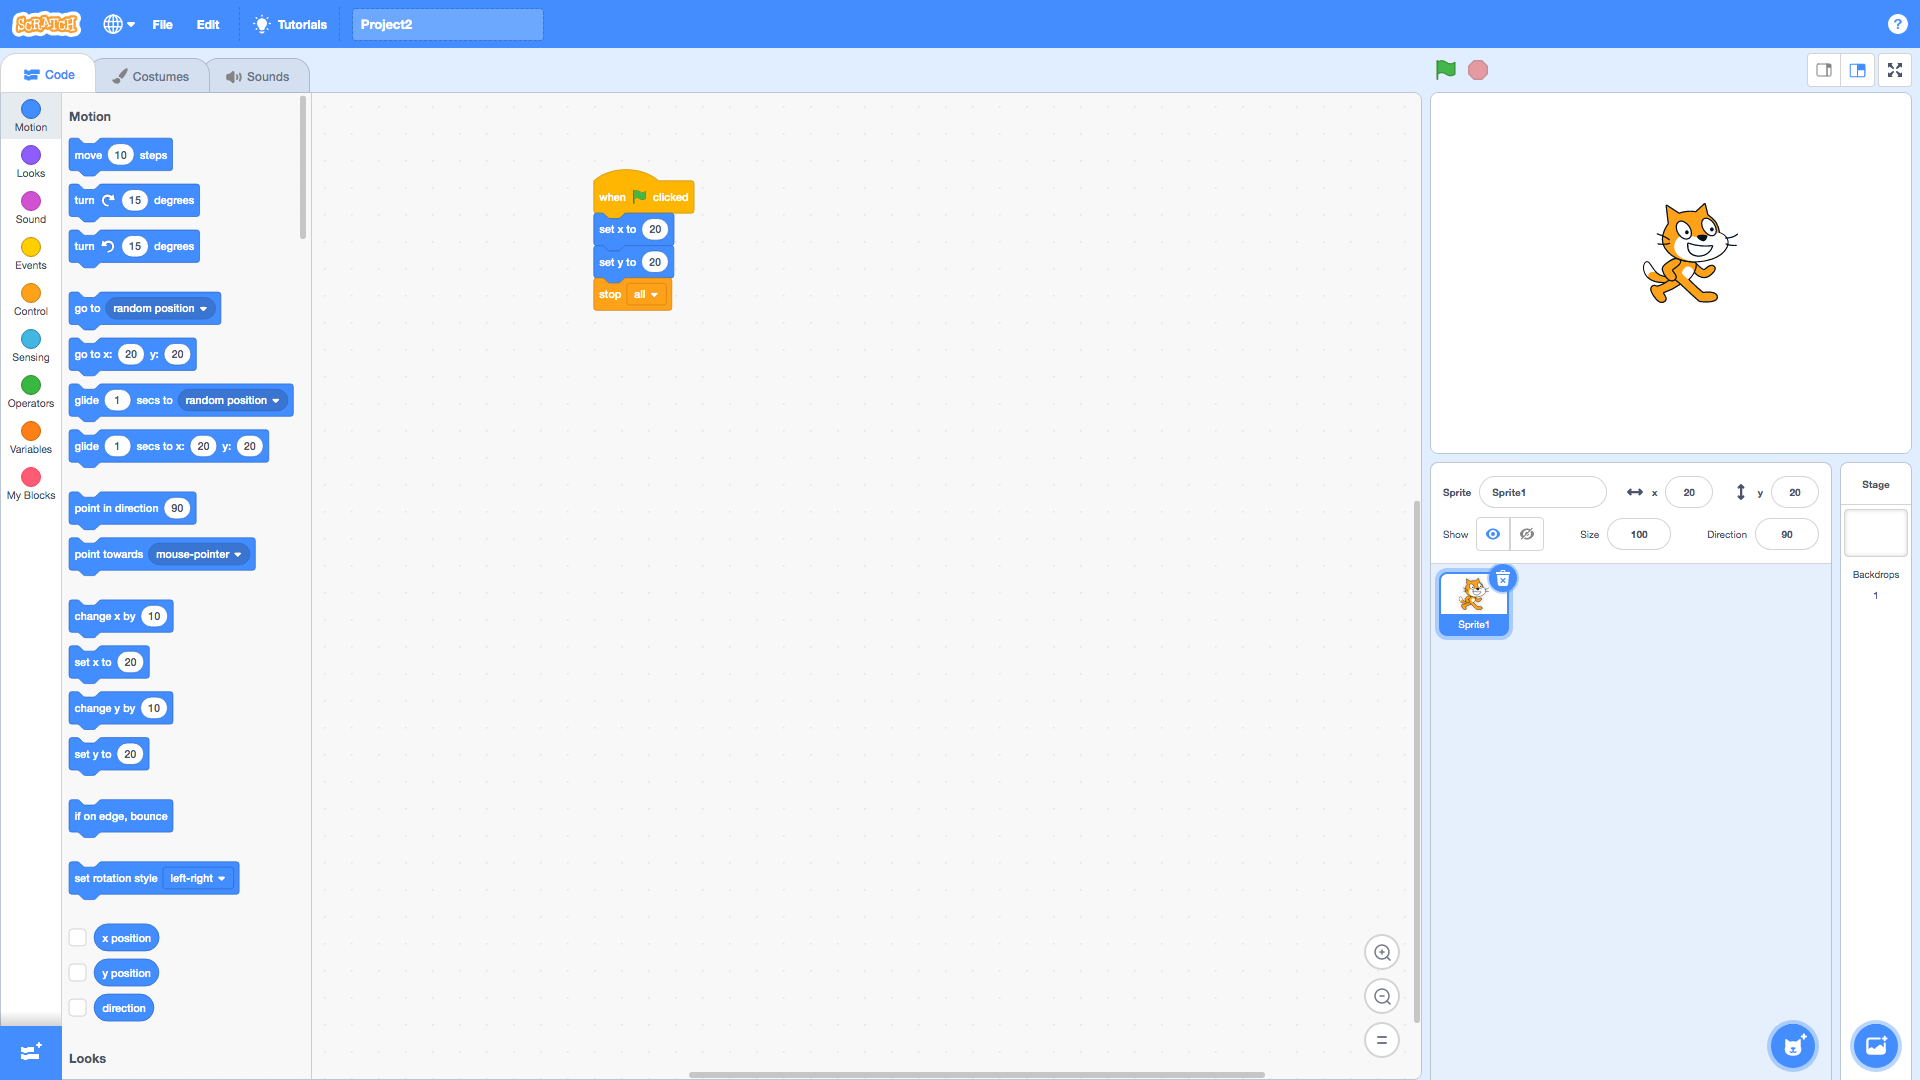
\includegraphics[width=1.0\linewidth,height=0.5\linewidth]{fig0065.png}
%  \caption{Последователна промяна на абсолютни координати}
%\label{fig0065}
%\end{figure}
%
%При своето движение, когато анимираният герой достигне границите на работното пространство, единият вариант е движението да продължи извън видимата зона. Другият вариант е да се вземат мерки и героят да отскача от ръбовете на работното пространство. За това отскачане има конкретно блокче (Фиг. \ref{fig0066}). За да се илюстрира работата му е нужна малко по-сложна последователност от инструкции. При всяко стартиране на програмата, първо се променят относителните координати, а след това се извършва отскачане от ръба, ако е необходимо. За да бъде малко по-интересен сценарият за проверка, вместо фиксирани стойности за относително отместване се използва вграждане на едно от зелените блокчета, което позволява генериране на случайно число в предварително определен диапазон. Съществено е да се забележи, че зеленото блокче има овална форма, което подсказва, че то е предназначено за вграждане в някой от другите блокове, които имат овален слот. 
%
%\begin{figure}[H]
%  \centering
%  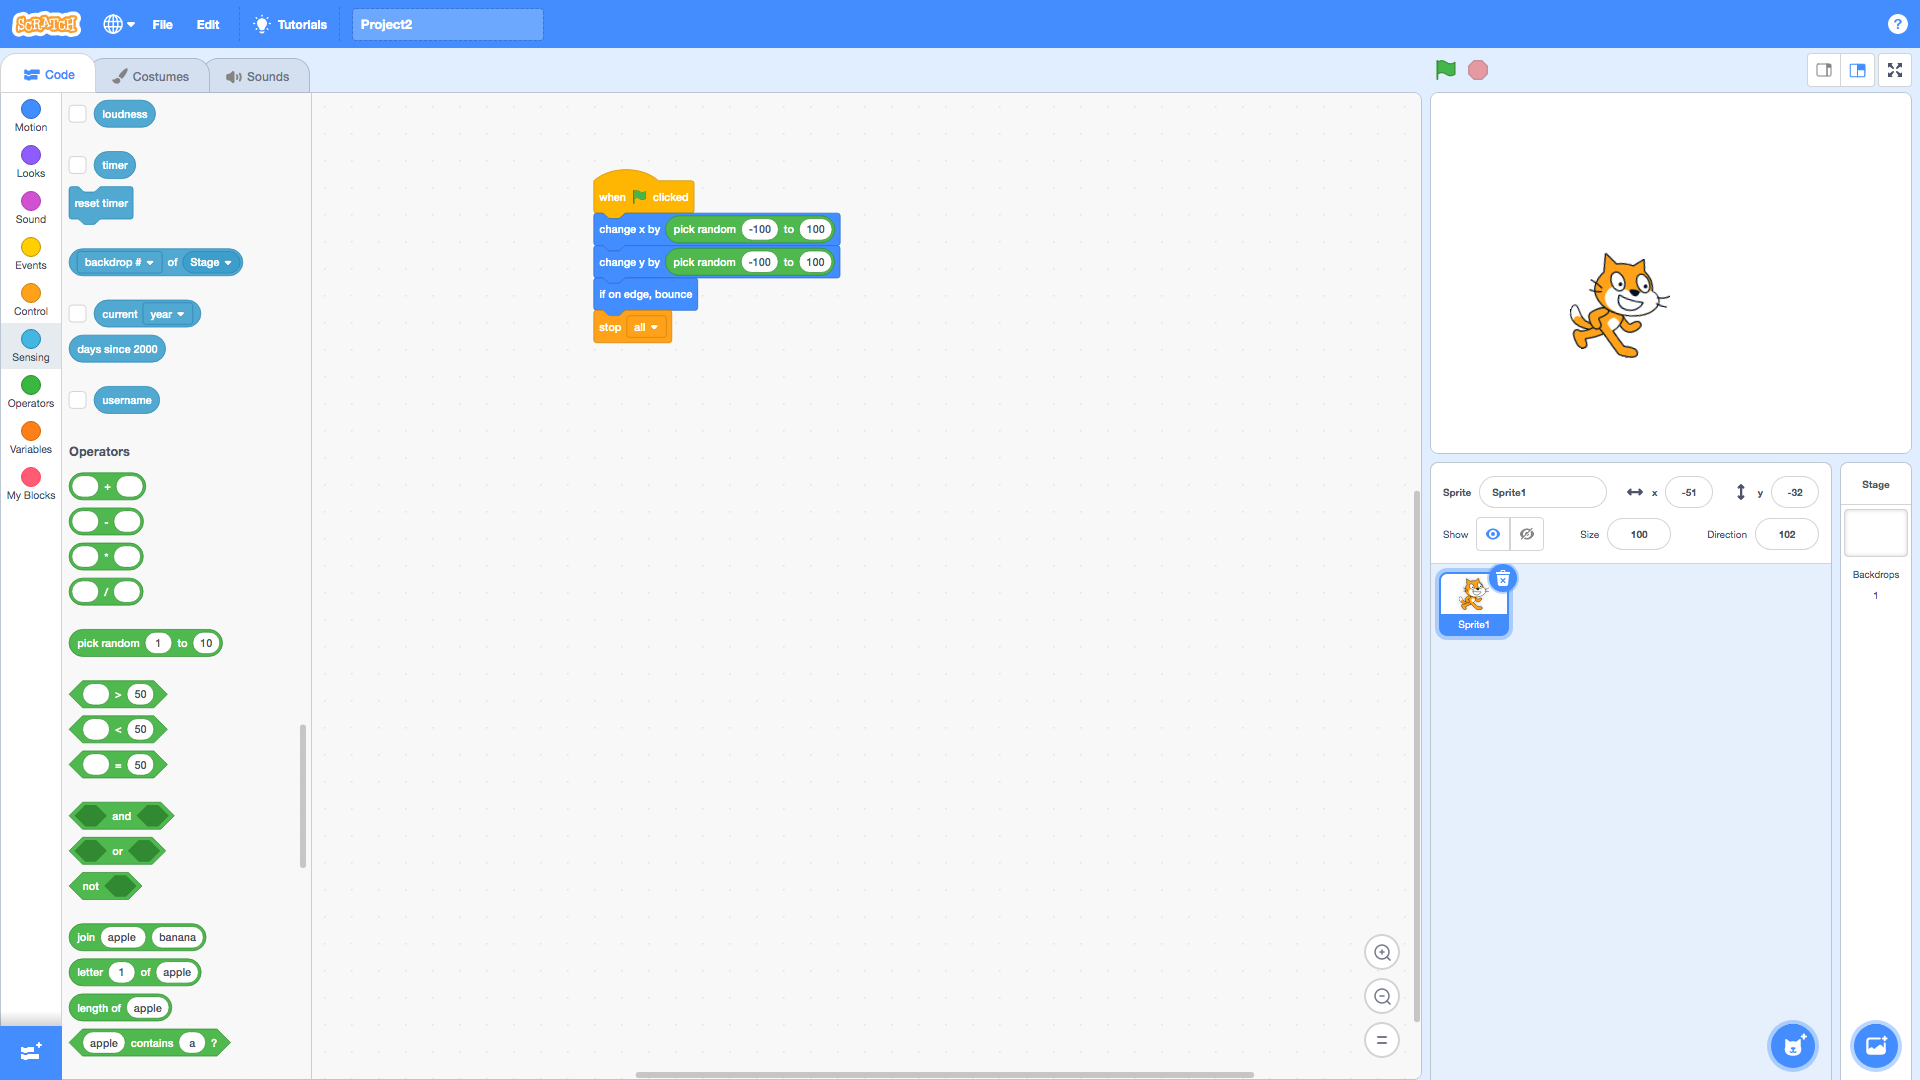
\includegraphics[width=1.0\linewidth,height=0.5\linewidth]{fig0066.png}
%  \caption{Отскачане от ръбовете}
%\label{fig0066}
%\end{figure}
%
%Следващо, много полезно блокче, от групата на тъмно оранжевите е блокчето за изчакване на период от време (Фиг. \ref{fig0067}). Когато това блокче бъде поставено между блокчетата за начало и край, програмата изчаква зададения брой секунди, преди да преустанови изпълнението си. По време на изпълнение, ясно може да се забележи, че около последователността от инструкции се появява жълта рамка, която символизира режима на изпълняващи се инструкции. 
%
%\begin{figure}[H]
%  \centering
%  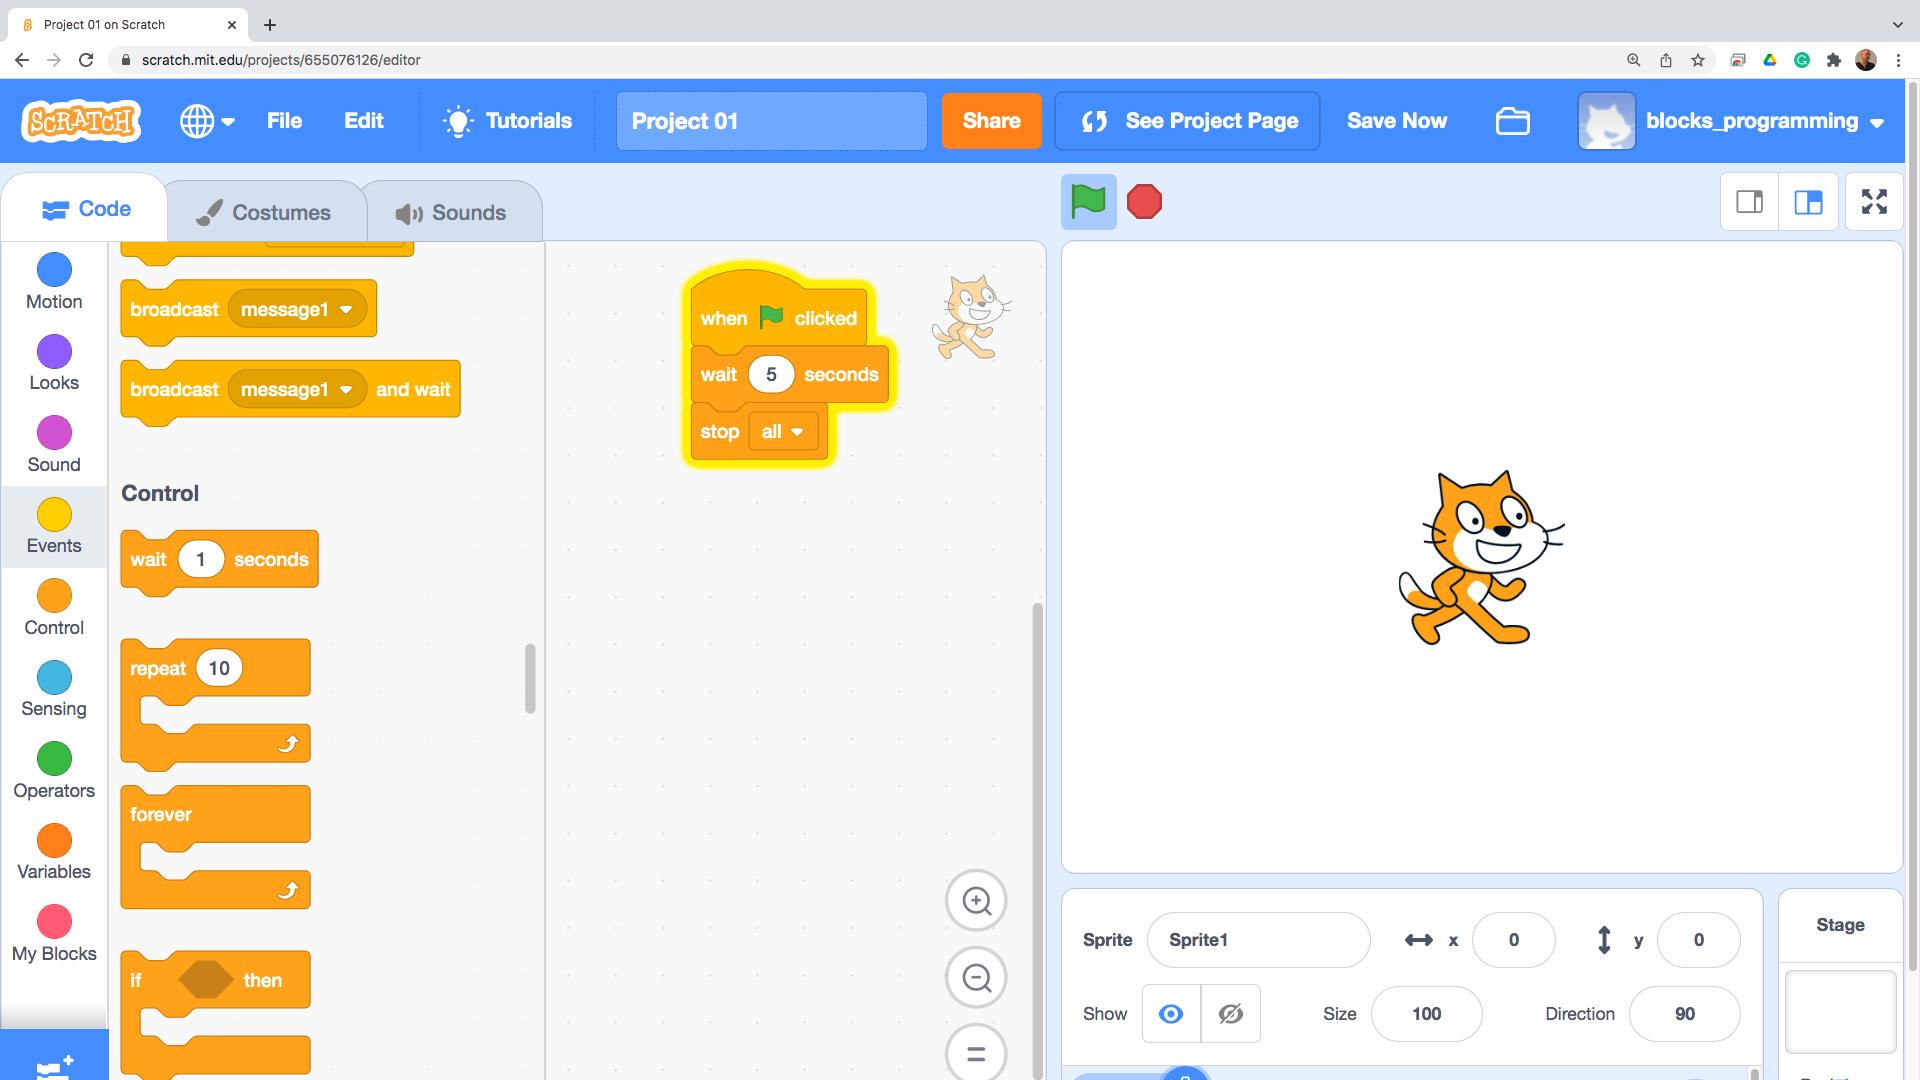
\includegraphics[width=1.0\linewidth,height=0.5\linewidth]{fig0067.png}
%  \caption{Инструкция за изчакване}
%\label{fig0067}
%\end{figure}
%
%Групата на лилавите блокчета съдържат инструкции за външното оформление на анимирания герой. Първите две блокчета са предназначени за реплики (Фиг. \ref{fig0068}), които героят казва (изписват се както в комикс). Първото блокче задава текст, който стои на екрана до следващата инструкция. Точно за това е нужно да има няколко секунди изчакване, така че текстът да остане видим за потребителя. Второто блокче има и параметър с който да се определи колко секунди текстът да бъде видим за потребителя. 
%
%\begin{figure}[H]
%  \centering
%  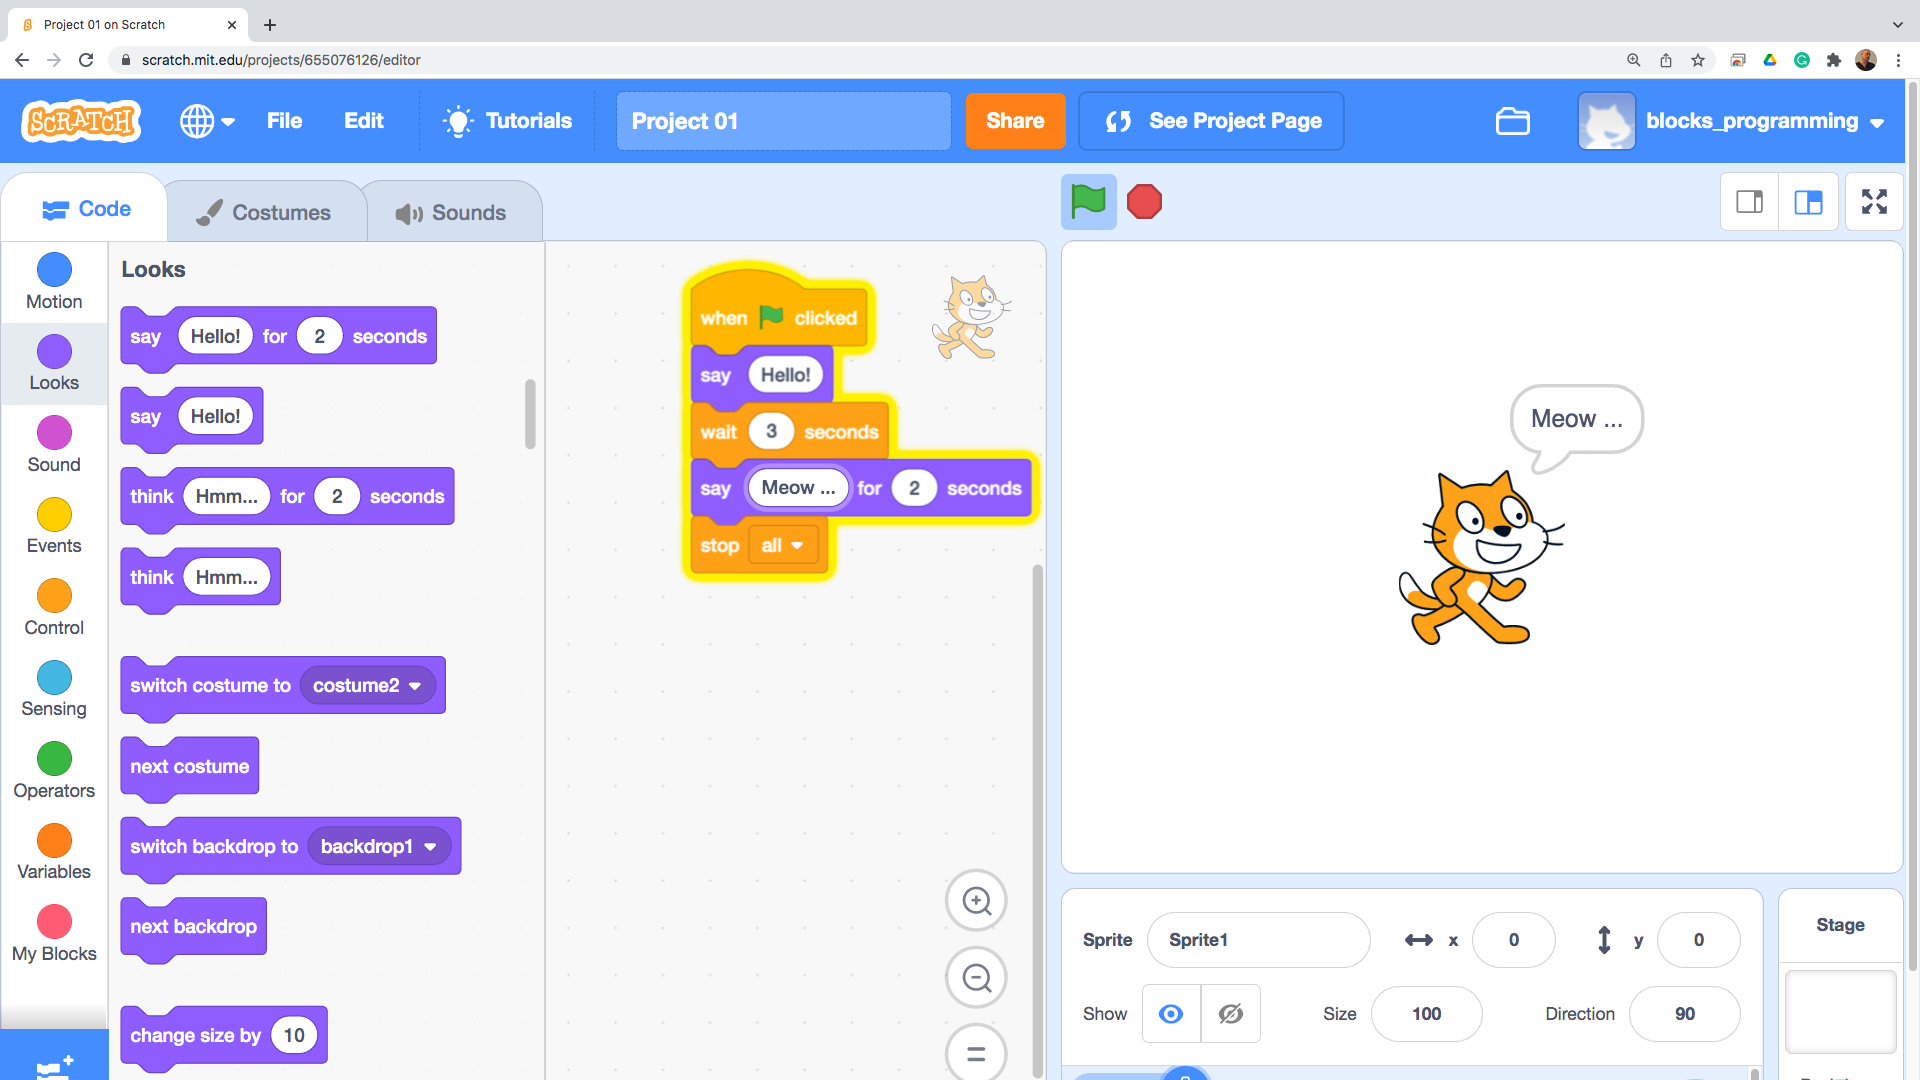
\includegraphics[width=1.0\linewidth,height=0.5\linewidth]{fig0068.png}
%  \caption{Изписване на реплики за изговаряне}
%\label{fig0068}
%\end{figure}
%
%Вторите две блокчета са предвидени за реплики, които анимираният герой си мисли, но не изрича. Разликата се състои в начина по който се визуализира текстът (Фиг. \ref{fig0069}).
%
%\begin{figure}[H]
%  \centering
%  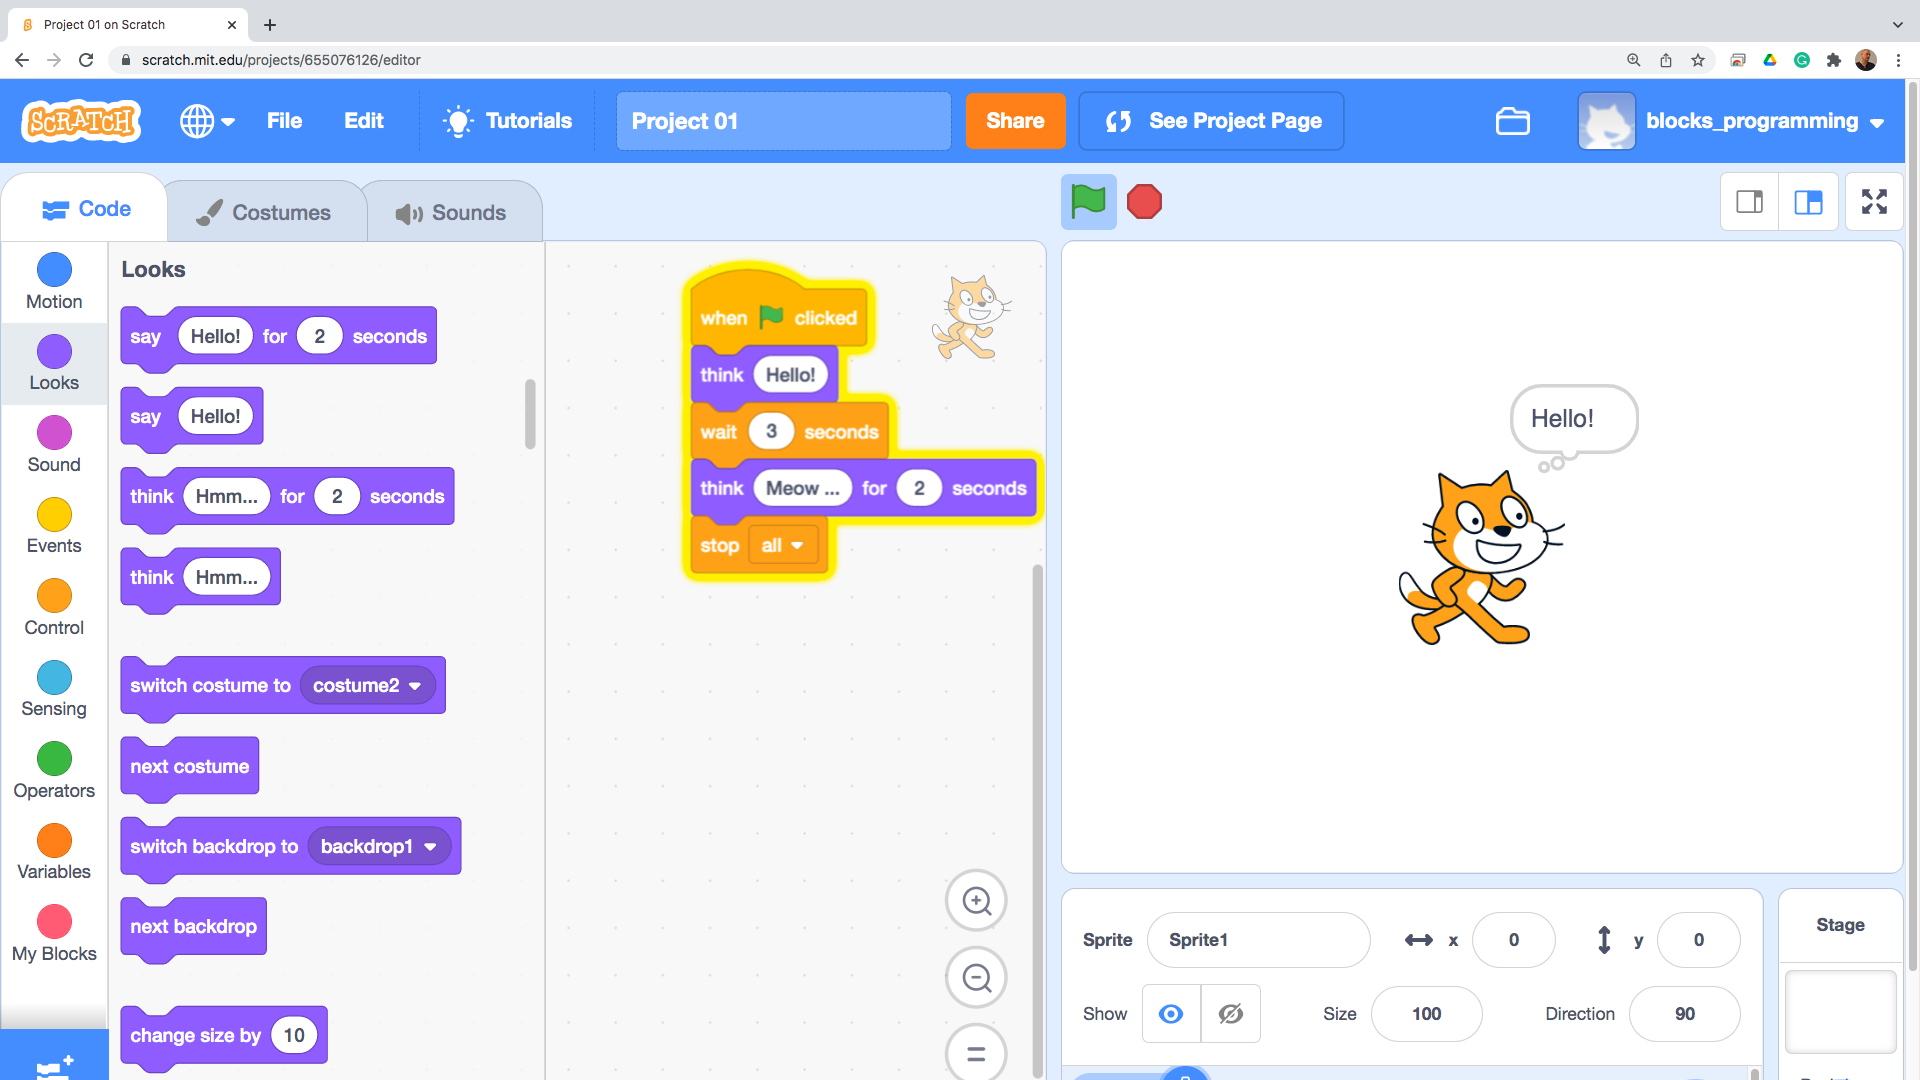
\includegraphics[width=1.0\linewidth,height=0.5\linewidth]{fig0069.png}
%  \caption{Изписване на реплики, като мисъл}
%\label{fig0069}
%\end{figure}
%
%Анимираните герои в Scratch са под формата на спрайтове. Спрайтът е набор от различни изображения за героя в различни пози. За смяната на тези различни пози се използват две блокчета (Фиг. \ref{fig0070}), като първото задава конкретен кадър в спрайта, а второто задава следващия кадър в последователността.
%
%\begin{figure}[H]
%  \centering
%  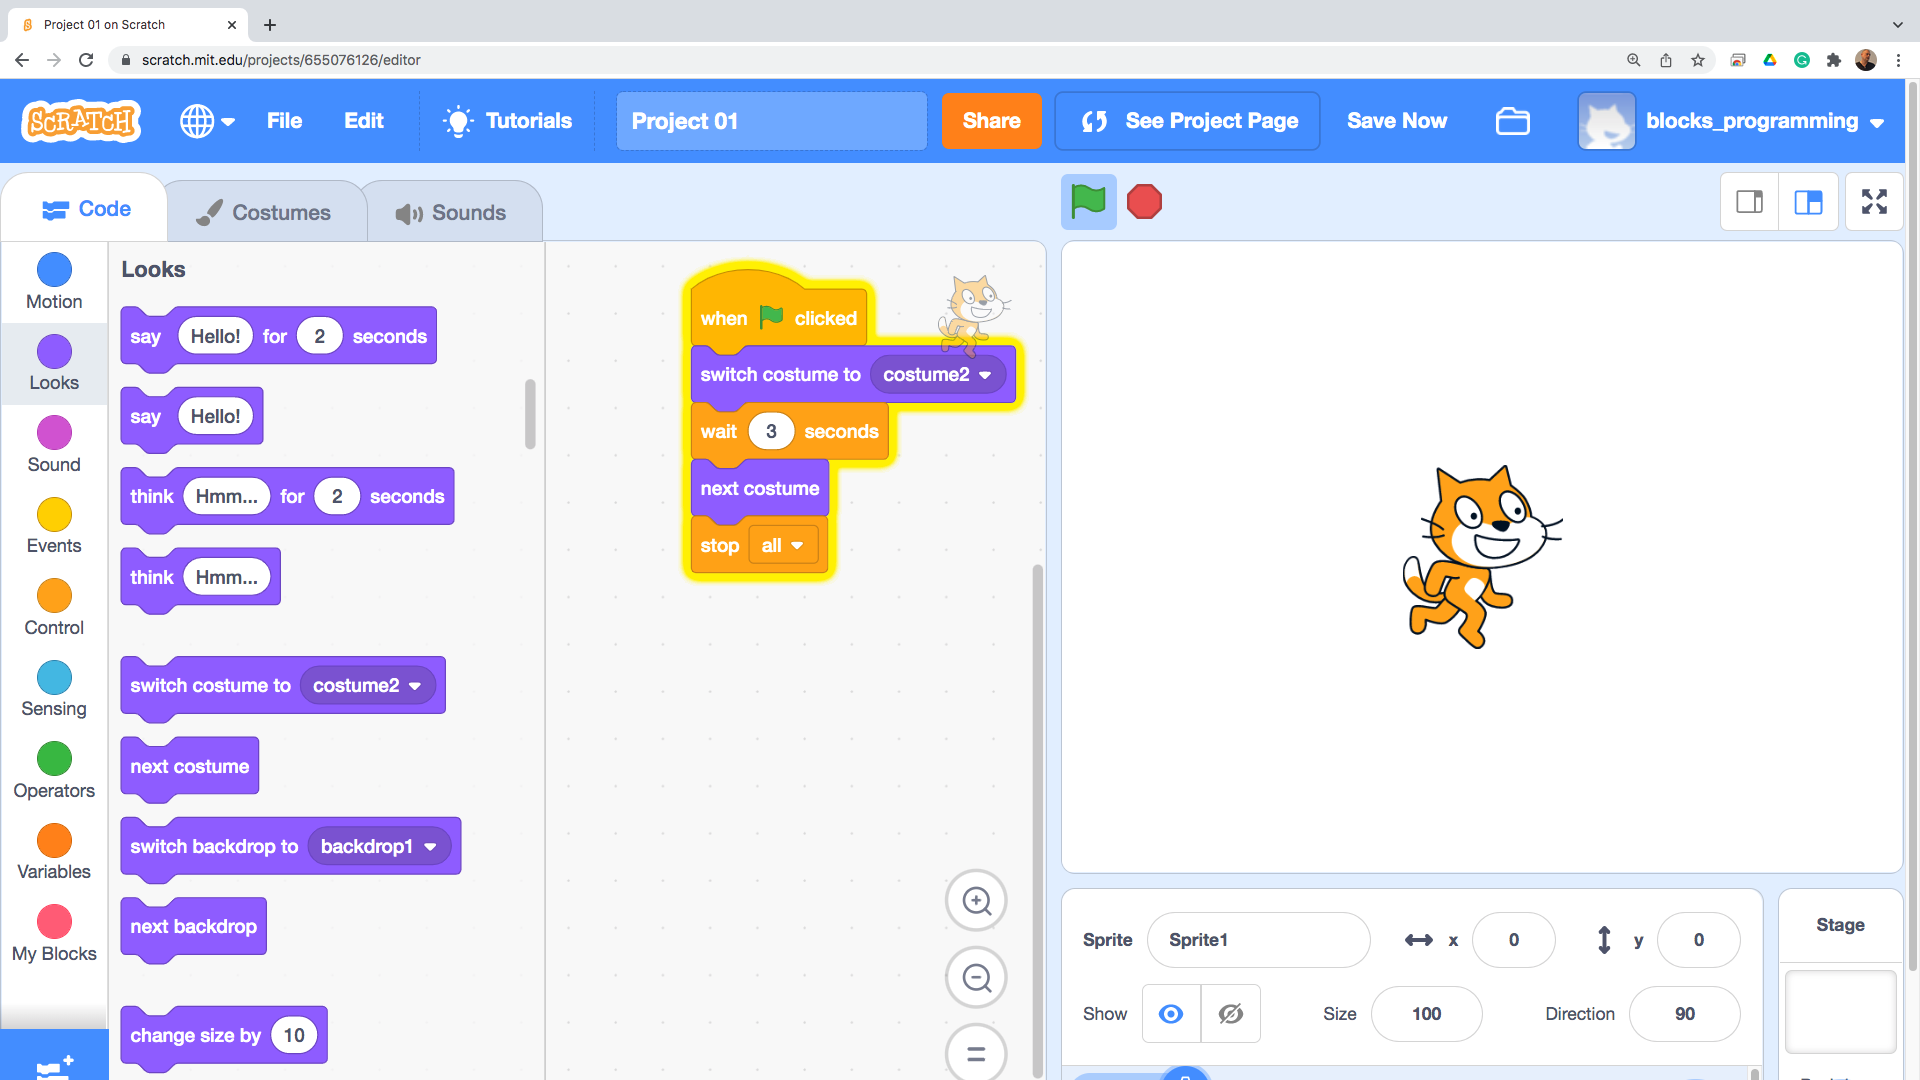
\includegraphics[width=1.0\linewidth,height=0.5\linewidth]{fig0070.png}
%  \caption{Смяна на пози}
%\label{fig0070}
%\end{figure}
%
%На работната сцена освен анимираните герои (под формата на спрайтове) има и фоново изображение. Това фоново изображение също подлежи на промяна, за което са предвидени две отделни блочета (Фиг. \ref{fig0071}). С първото може да се избират фонови изображения напред, назад, по случаен принцип или с конкретно название, а с второто блокче следващото изображение в последователността. 
%
%\begin{figure}[H]
%  \centering
%  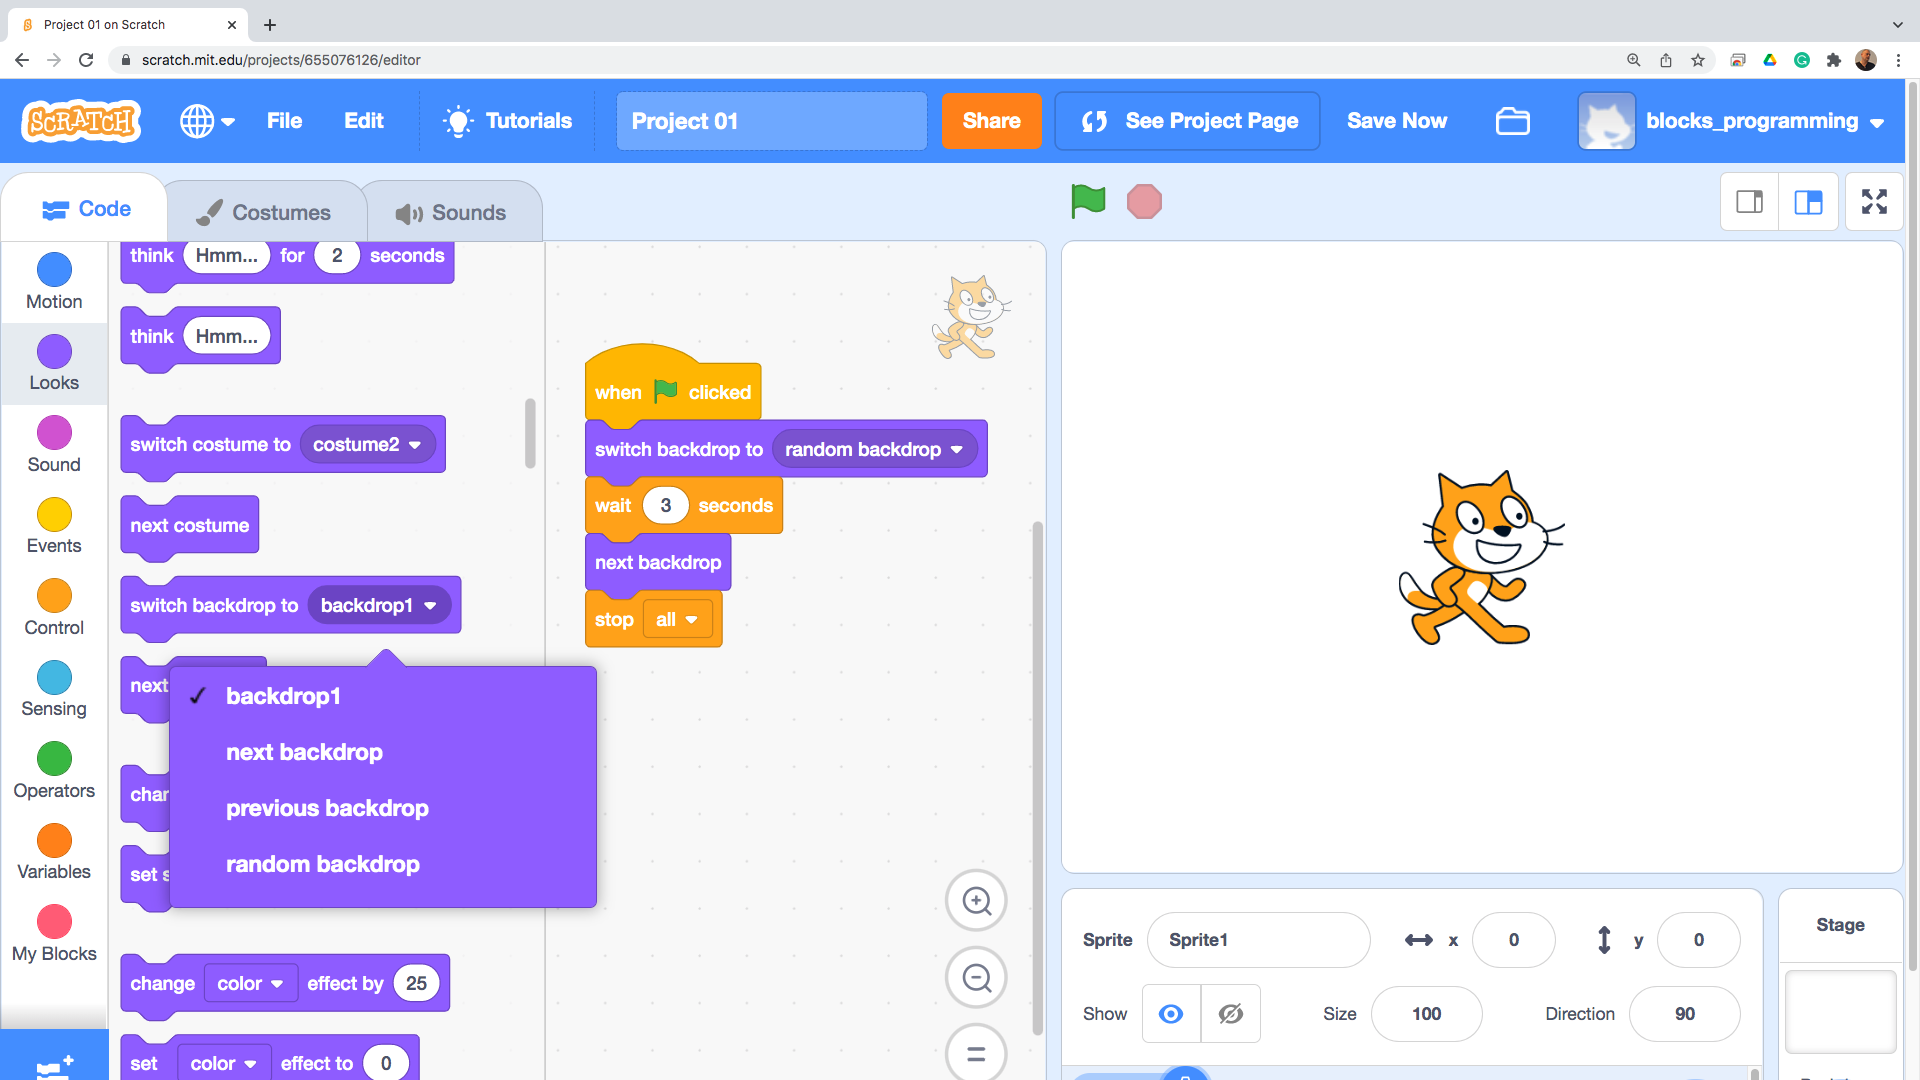
\includegraphics[width=1.0\linewidth,height=0.5\linewidth]{fig0071.png}
%  \caption{Смяна на фона}
%\label{fig0071}
%\end{figure}
%
%За промяната на размера на анимирания герой има две конкретни блокчета, като първото променя размера в абсолютни стойности, а второто променя размера в проценти, спрямо оригиналния размер (Фиг. \ref{fig0072}).
%
%\begin{figure}[H]
%  \centering
%  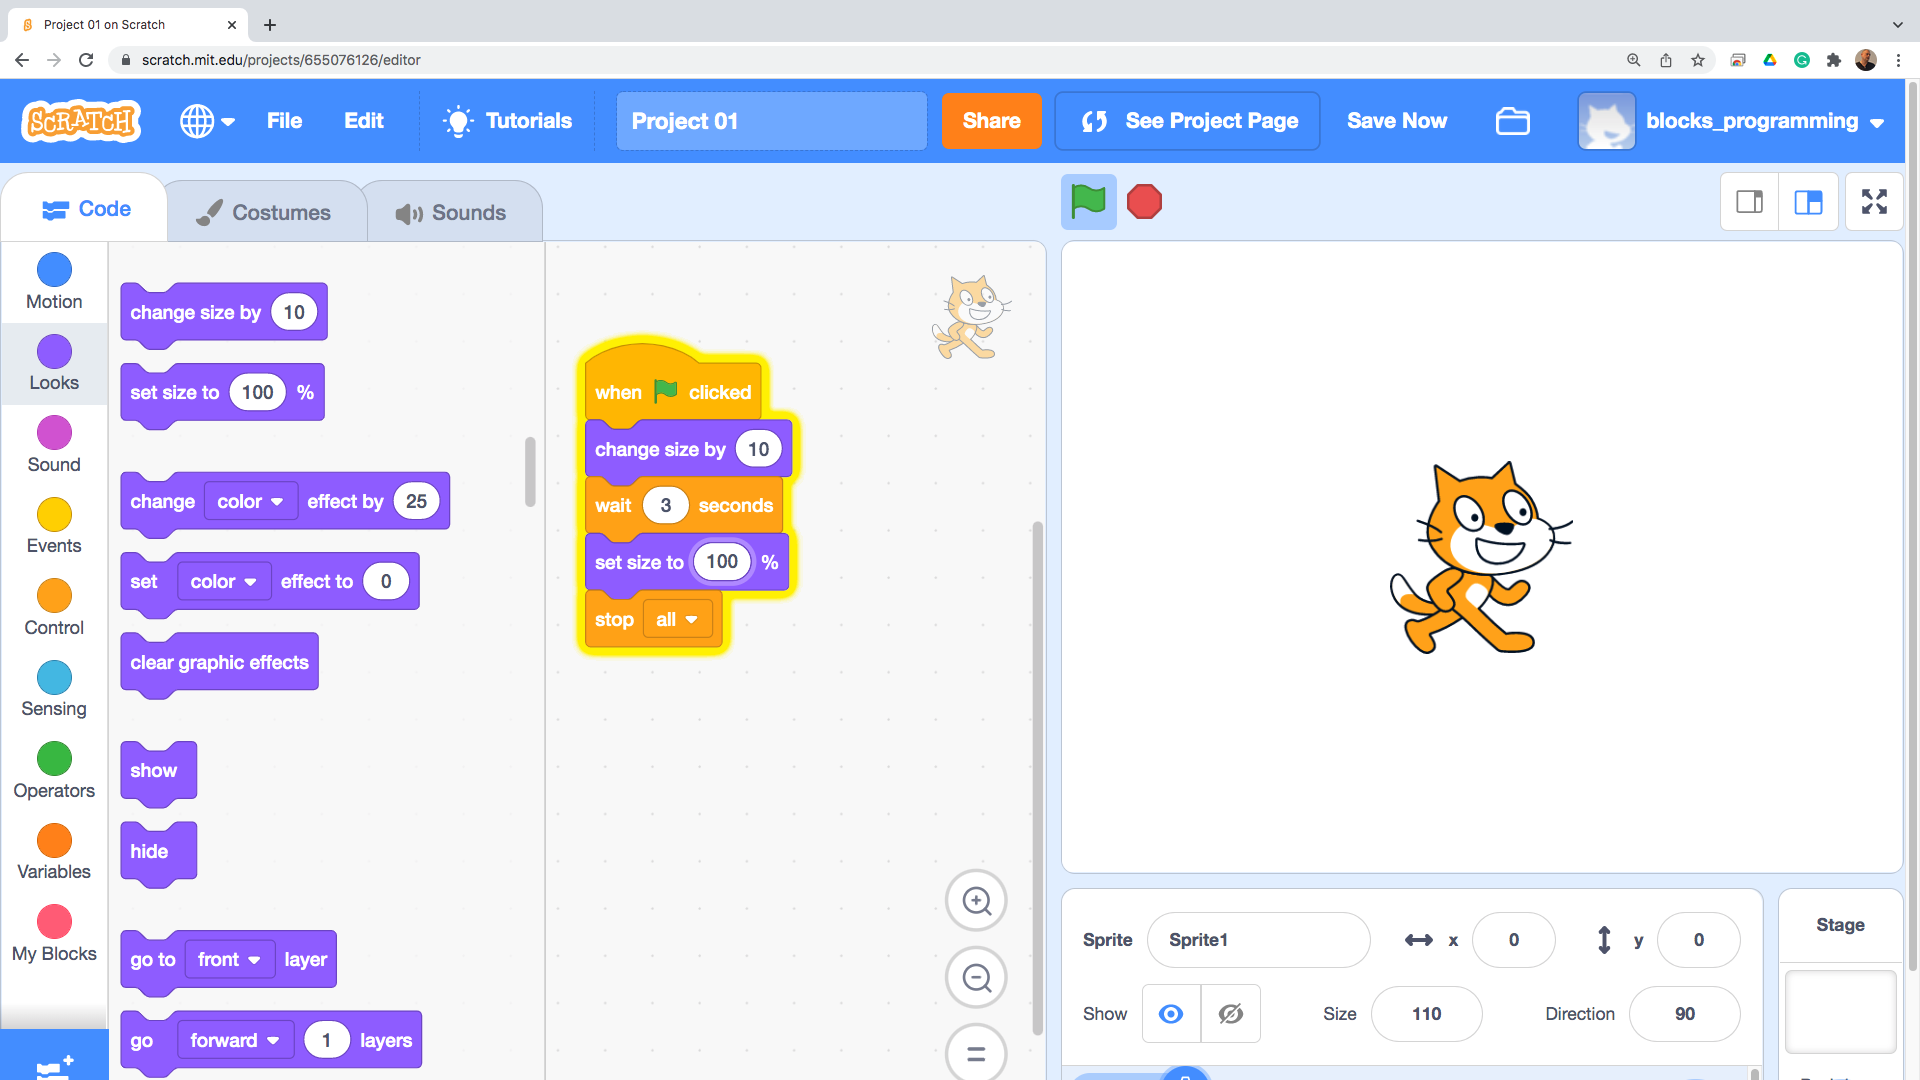
\includegraphics[width=1.0\linewidth,height=0.5\linewidth]{fig0072.png}
%  \caption{Промяна на размерите}
%\label{fig0072}
%\end{figure}
%
%За промяна на визуалното оформление на анимирания герой са предвидени три блокчета (Фиг. \ref{fig0073}). Първите две задават промяна, като промяната може да бъде в цвета, различни изкривявания, пикселизация, мозайка, прозрачност или яркост, а третото блокче отменя всички направени декорации. Първото блокче предизвиква относителна промяна, спрямо текущото състояние на героя, а второто блокче задава абсолютна промяна. Отново е важно да се дадат няколко секунди, така че промените да бъдат ясно различими. 
%
%\begin{figure}[H]
%  \centering
%  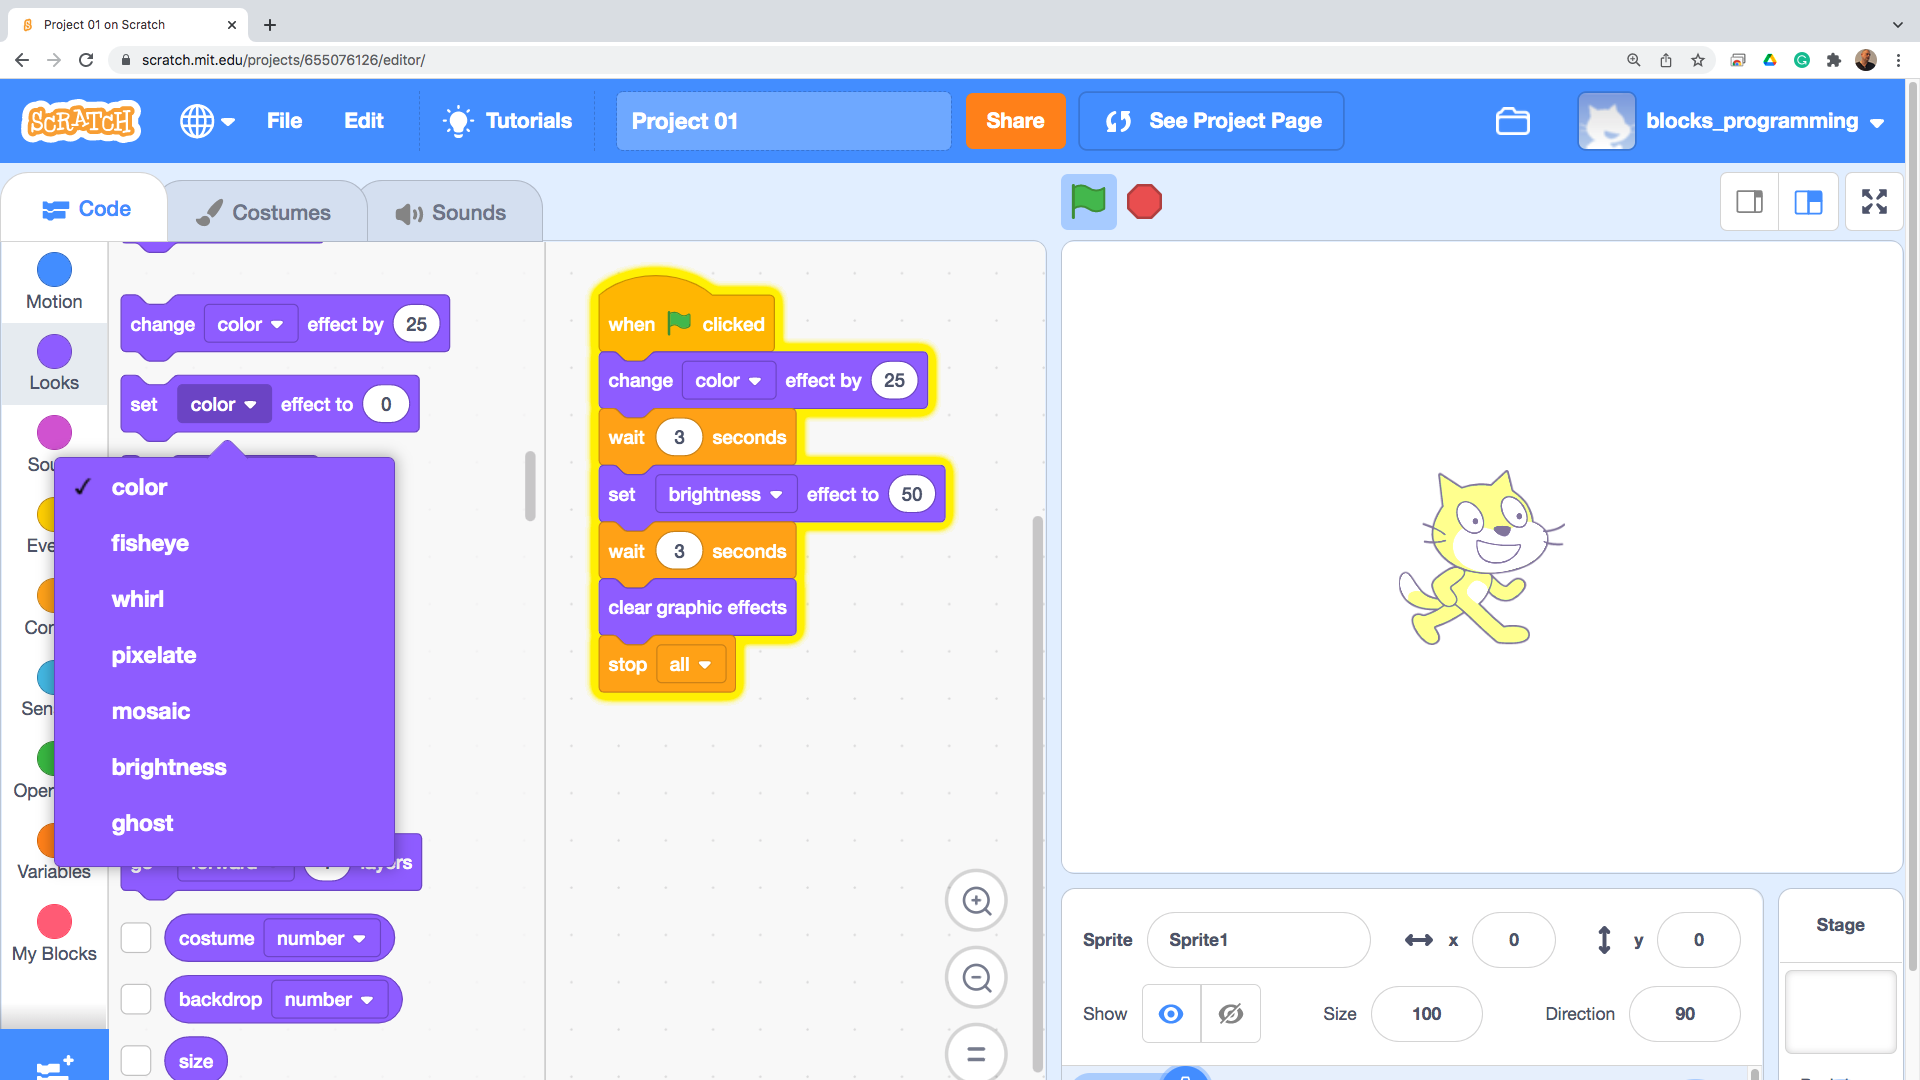
\includegraphics[width=1.0\linewidth,height=0.5\linewidth]{fig0073.png}
%  \caption{Промяна на външния вид}
%\label{fig0073}
%\end{figure}
%
%Работата със спрайтове е предимно за постигане на анимирани ефекти. Различните анимирани герой в сцената имат определени взаимодействия по между си. Сценарият на изработвания проект определя в кой момент всеки от героите се появява на сцената и в кой момент изчезва. За да се осъществи появата и изчезването са предвидени две блокчета, извършващи тези действия (Фиг. \ref{fig0074}).
%
%\begin{figure}[H]
%  \centering
%  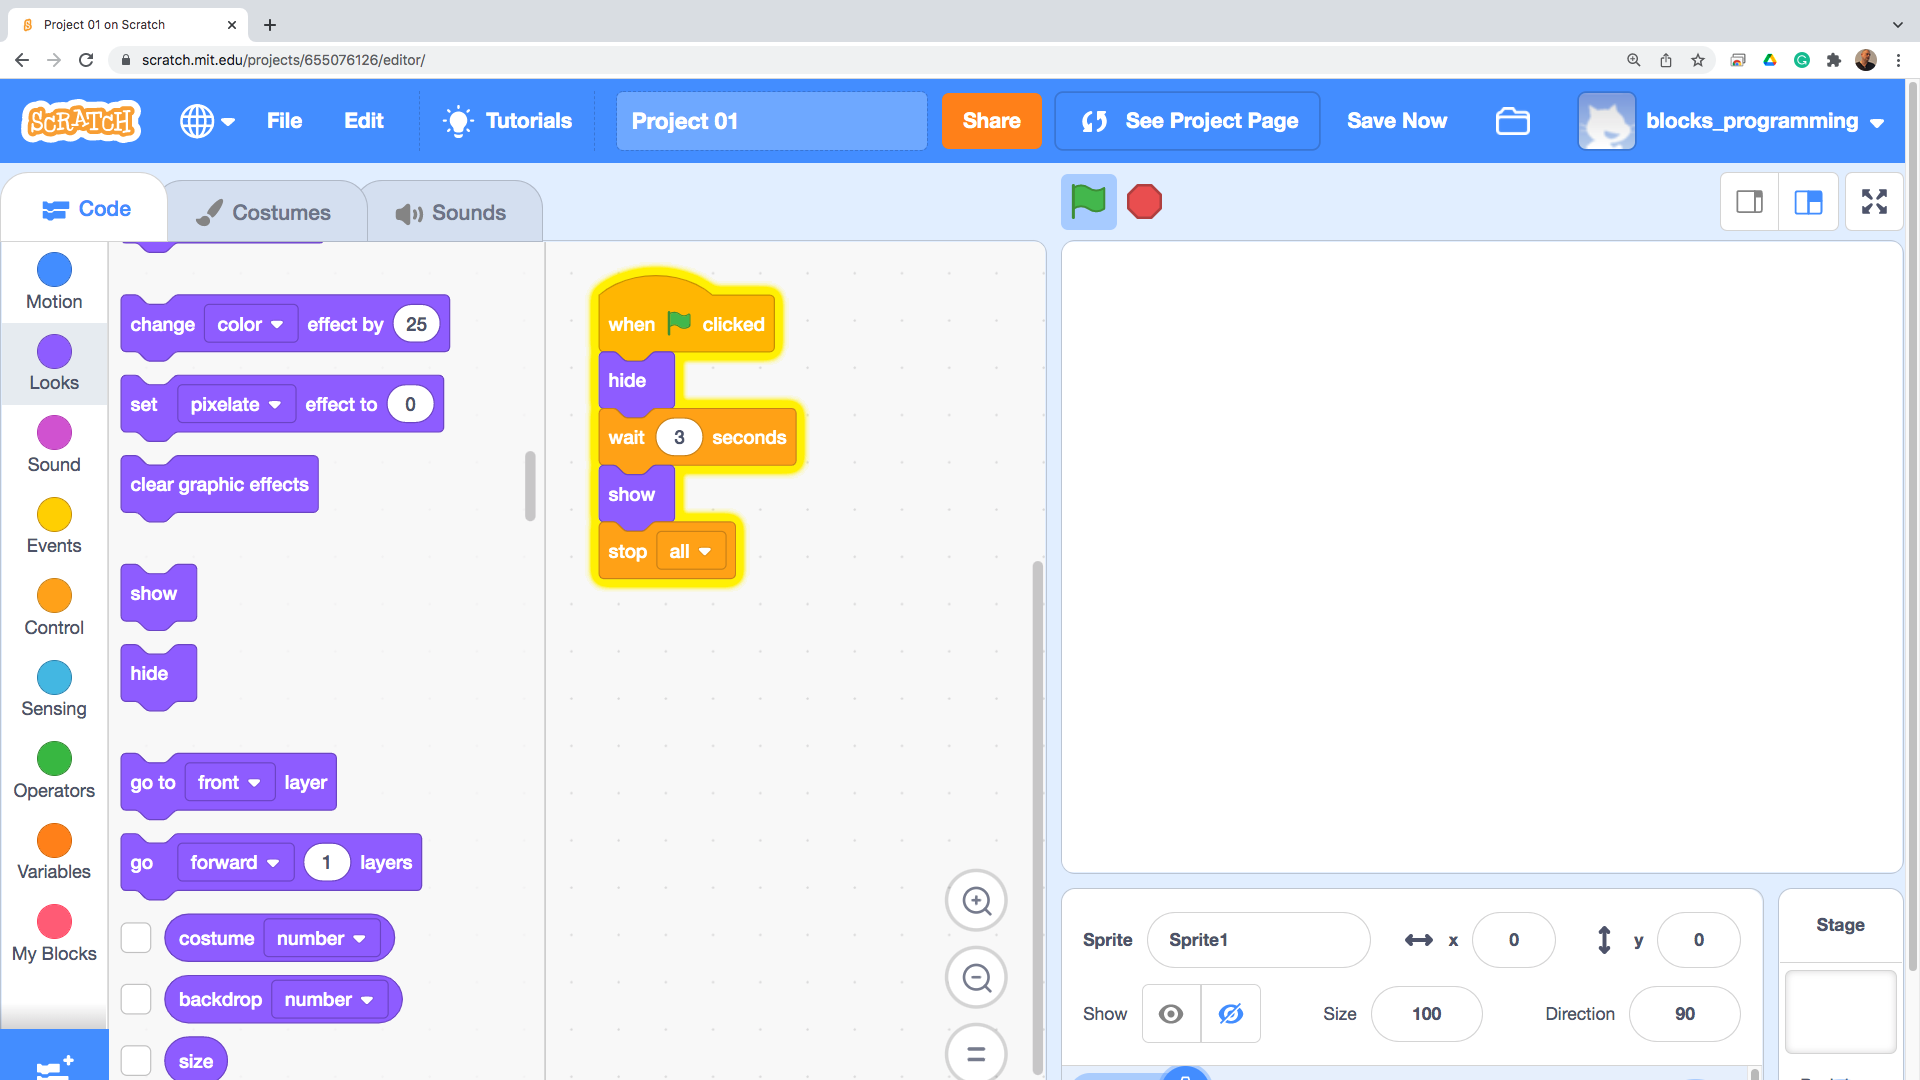
\includegraphics[width=1.0\linewidth,height=0.5\linewidth]{fig0074.png}
%  \caption{Скриване и повява}
%\label{fig0074}
%\end{figure}
%
%Множество програмни продукти, работещи с растерни графични изображения, организират различните изображения в слоеве. Пример за такива са Adobe Photoshop, GIMP, Microsoft Word, LibreOffice Draw и много други. Организацията в слоеве е логична, тъй като различните спрайтове в определени моменти от времето могат да се припокриват. В някои от софтуерните пакети за графична обработка, наличието на слоеве се възприема като Z буфер. В Scratch също е налична възможността за работа със слоеве, като две конкретни блокчета позволяват спрайтът да се придвижва напред и назад по слоевете (Фиг. \ref{fig0075}).
%
%\begin{figure}[H]
%  \centering
%  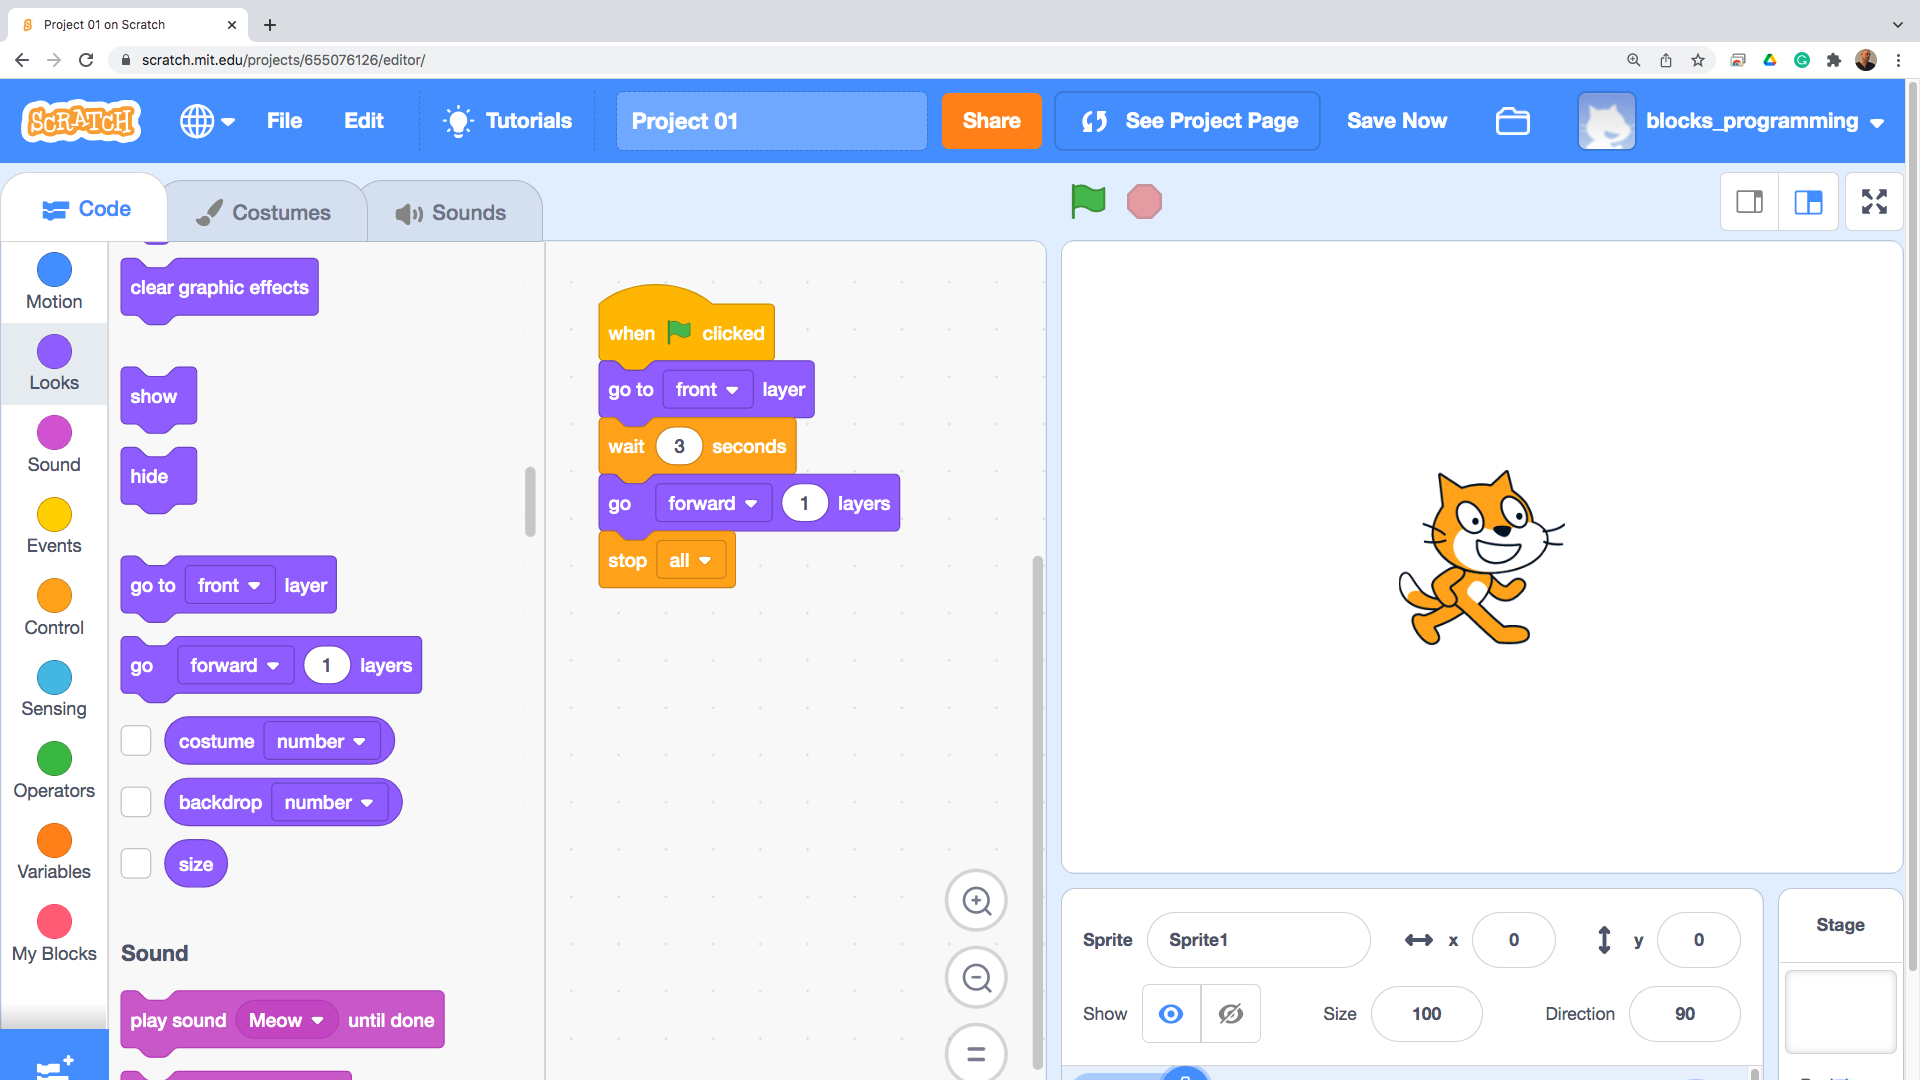
\includegraphics[width=1.0\linewidth,height=0.5\linewidth]{fig0075.png}
%  \caption{Придвижване по слоевете}
%\label{fig0075}
%\end{figure}
%
%Групата блокчета в пурпурен цвят са предназначени за звуково оформление. Изпълнението на звуци се постига с първите две блокчета в групата (Фиг. \ref{fig0076}). Първото блокче изпълнява звука докато той бъде приключен, а второто блокче го стартира и предава изпълнението към следващото блокче. С третото блокче всички изпълняващи се звуци биват спрени. Програмната среда позволява звуци да бъдат записани и от компютъра на потребителя. 
%
%\begin{figure}[H]
%  \centering
%  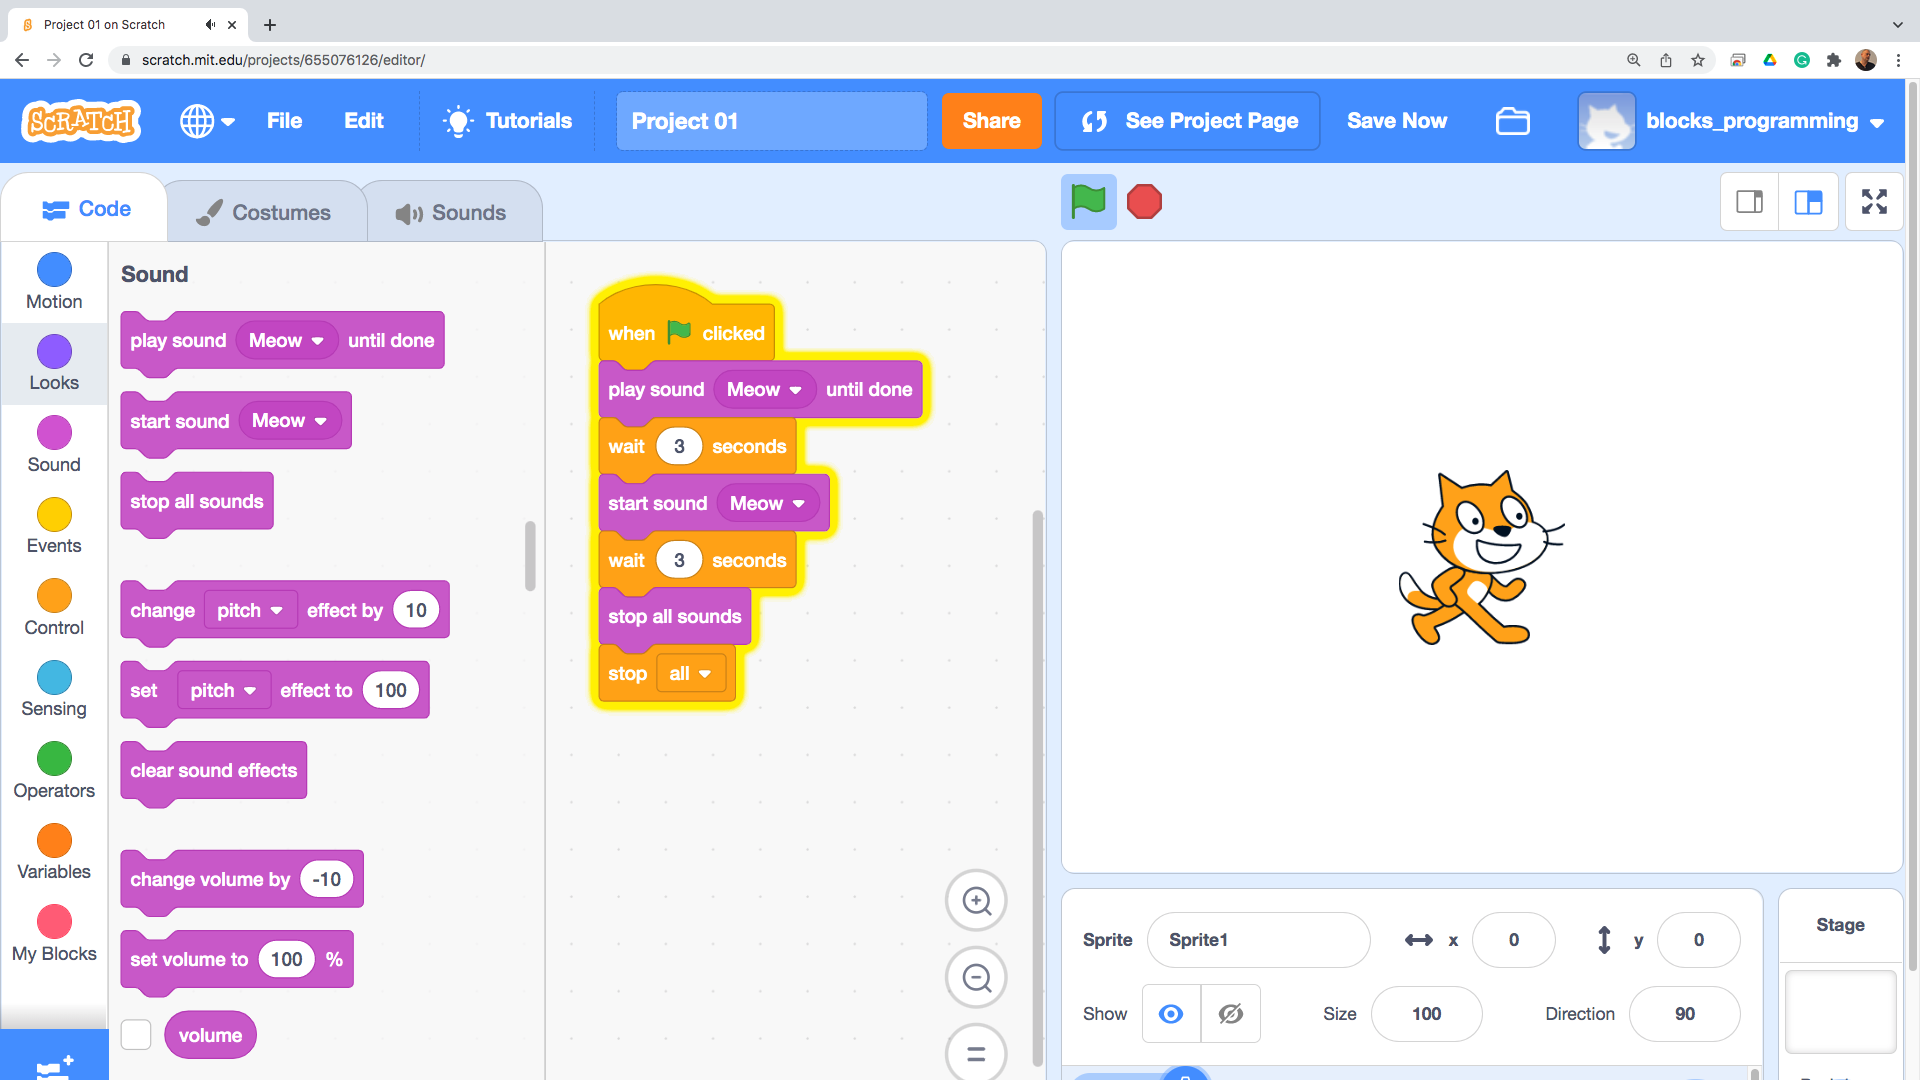
\includegraphics[width=1.0\linewidth,height=0.5\linewidth]{fig0076.png}
%  \caption{Изпълнение на звуци}
%\label{fig0076}
%\end{figure}
%
%Две от характеристиките на звуците могат да се променят с блокчетата за височина (честотна) и стерео озвучаване (ляво/дясно). И двете блокчета имат числени стойности за посочените характеристики (Фиг. \ref{fig0077}).
%
%\begin{figure}[H]
%  \centering
%  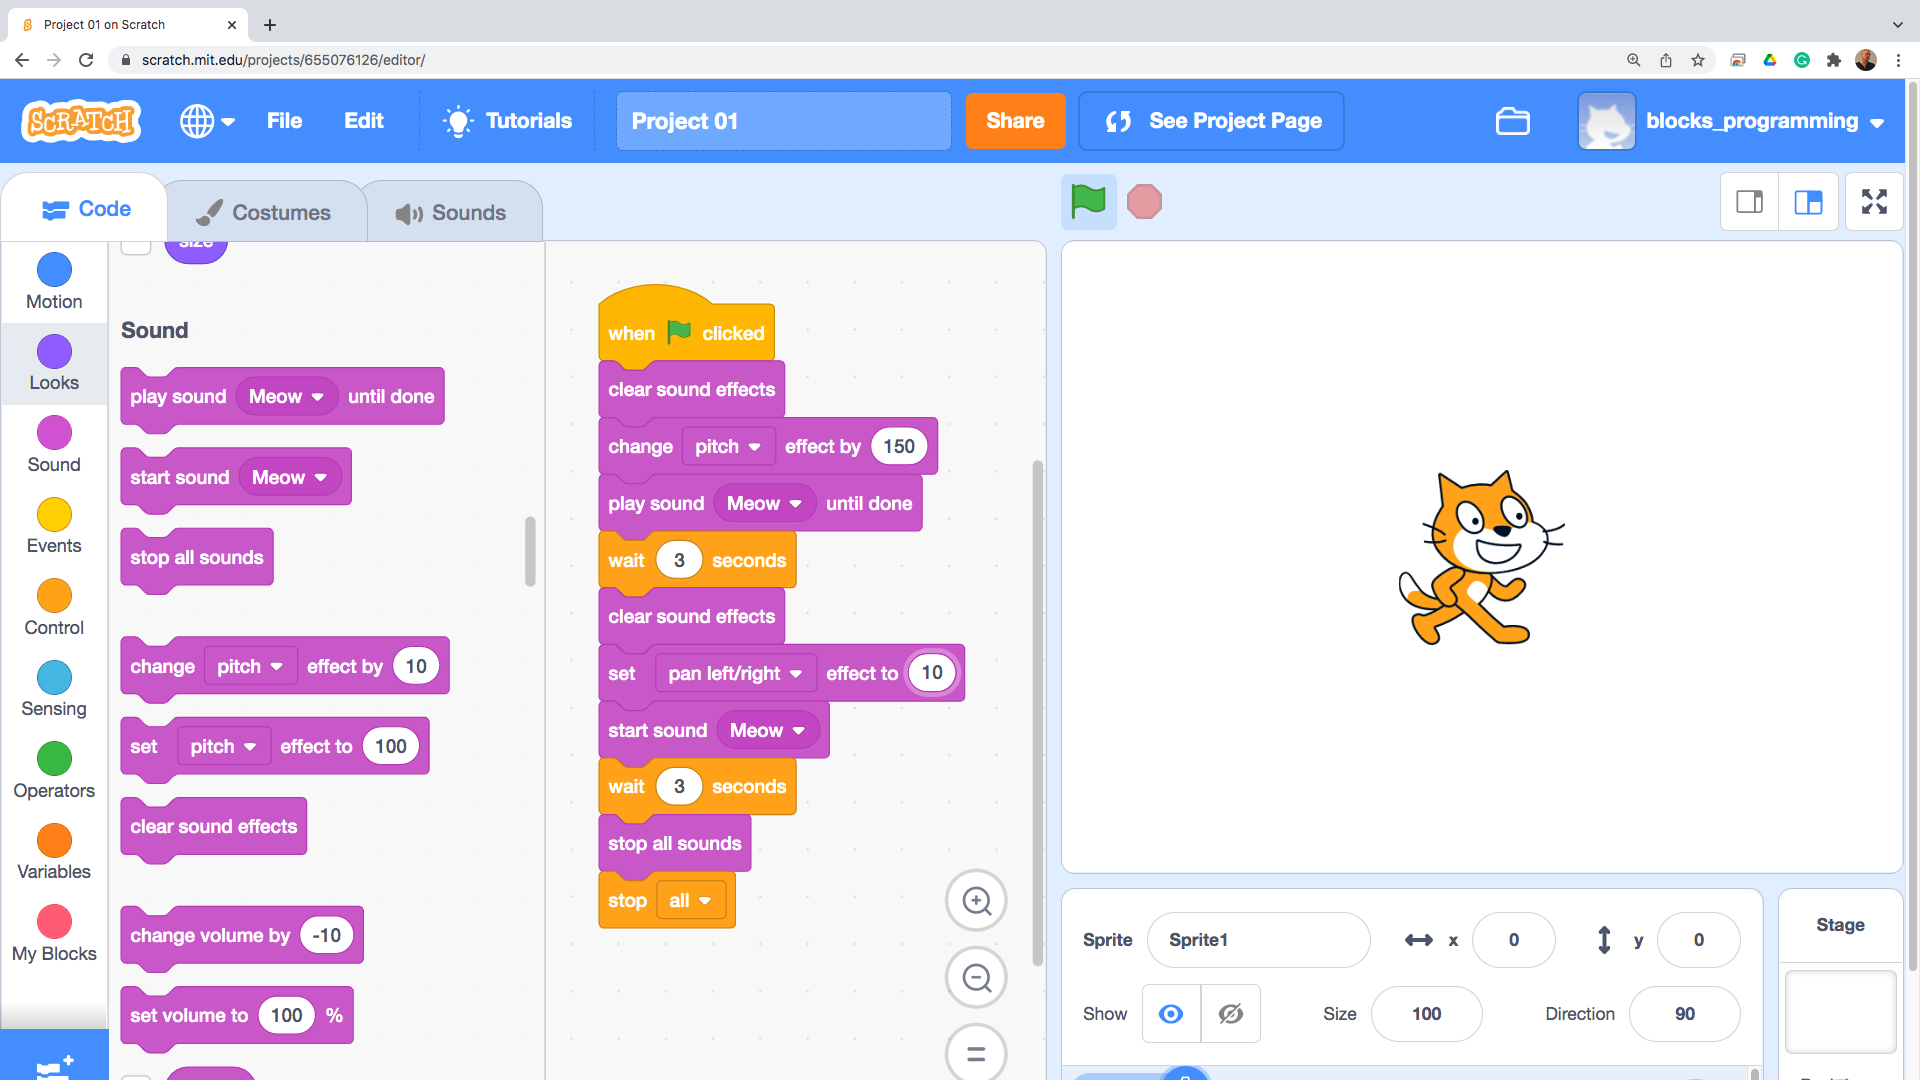
\includegraphics[width=1.0\linewidth,height=0.5\linewidth]{fig0077.png}
%  \caption{Характеристики на звука}
%\label{fig0077}
%\end{figure}
%
%За постигането на една по-богата звукова картина, силата на различните звуци може да се управлява с две блокчета (Фиг. \ref{fig0078}). Първото контролира силата на звука по абсолютна стойност, а второто като проценти. 
%
%\begin{figure}[H]
%  \centering
%  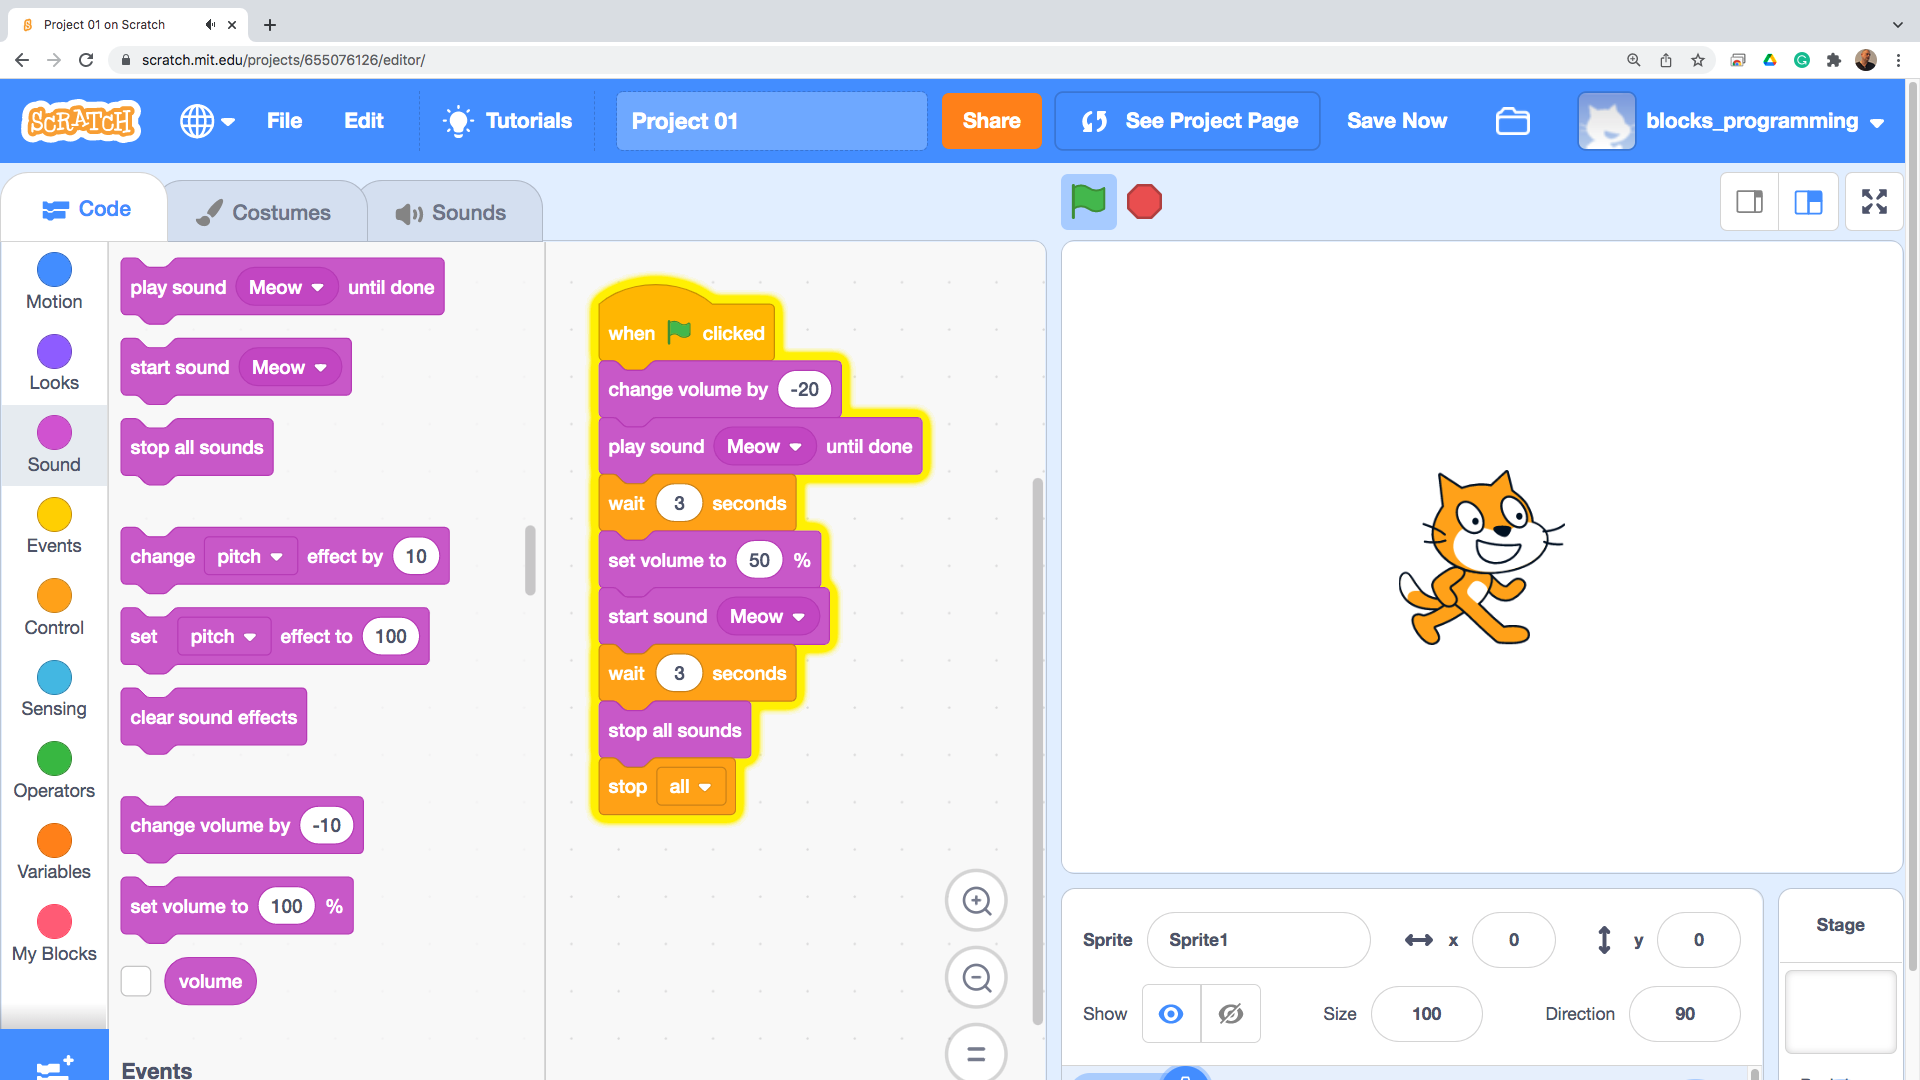
\includegraphics[width=1.0\linewidth,height=0.5\linewidth]{fig0078.png}
%  \caption{Сила на звука}
%\label{fig0078}
%\end{figure}
%
%Оранжевата група блокчета са предназначени за възникване на събития. Събитията са инструмент за изпълнение на инструкции, когато няма ясна престава за момента в който програмните инструкции трябва да се изпълнят. Такова събитие е натискане на бутон по клавиатурата от страна на потребителя (Фиг. \ref{fig0079}).
%
%\begin{figure}[H]
%  \centering
%  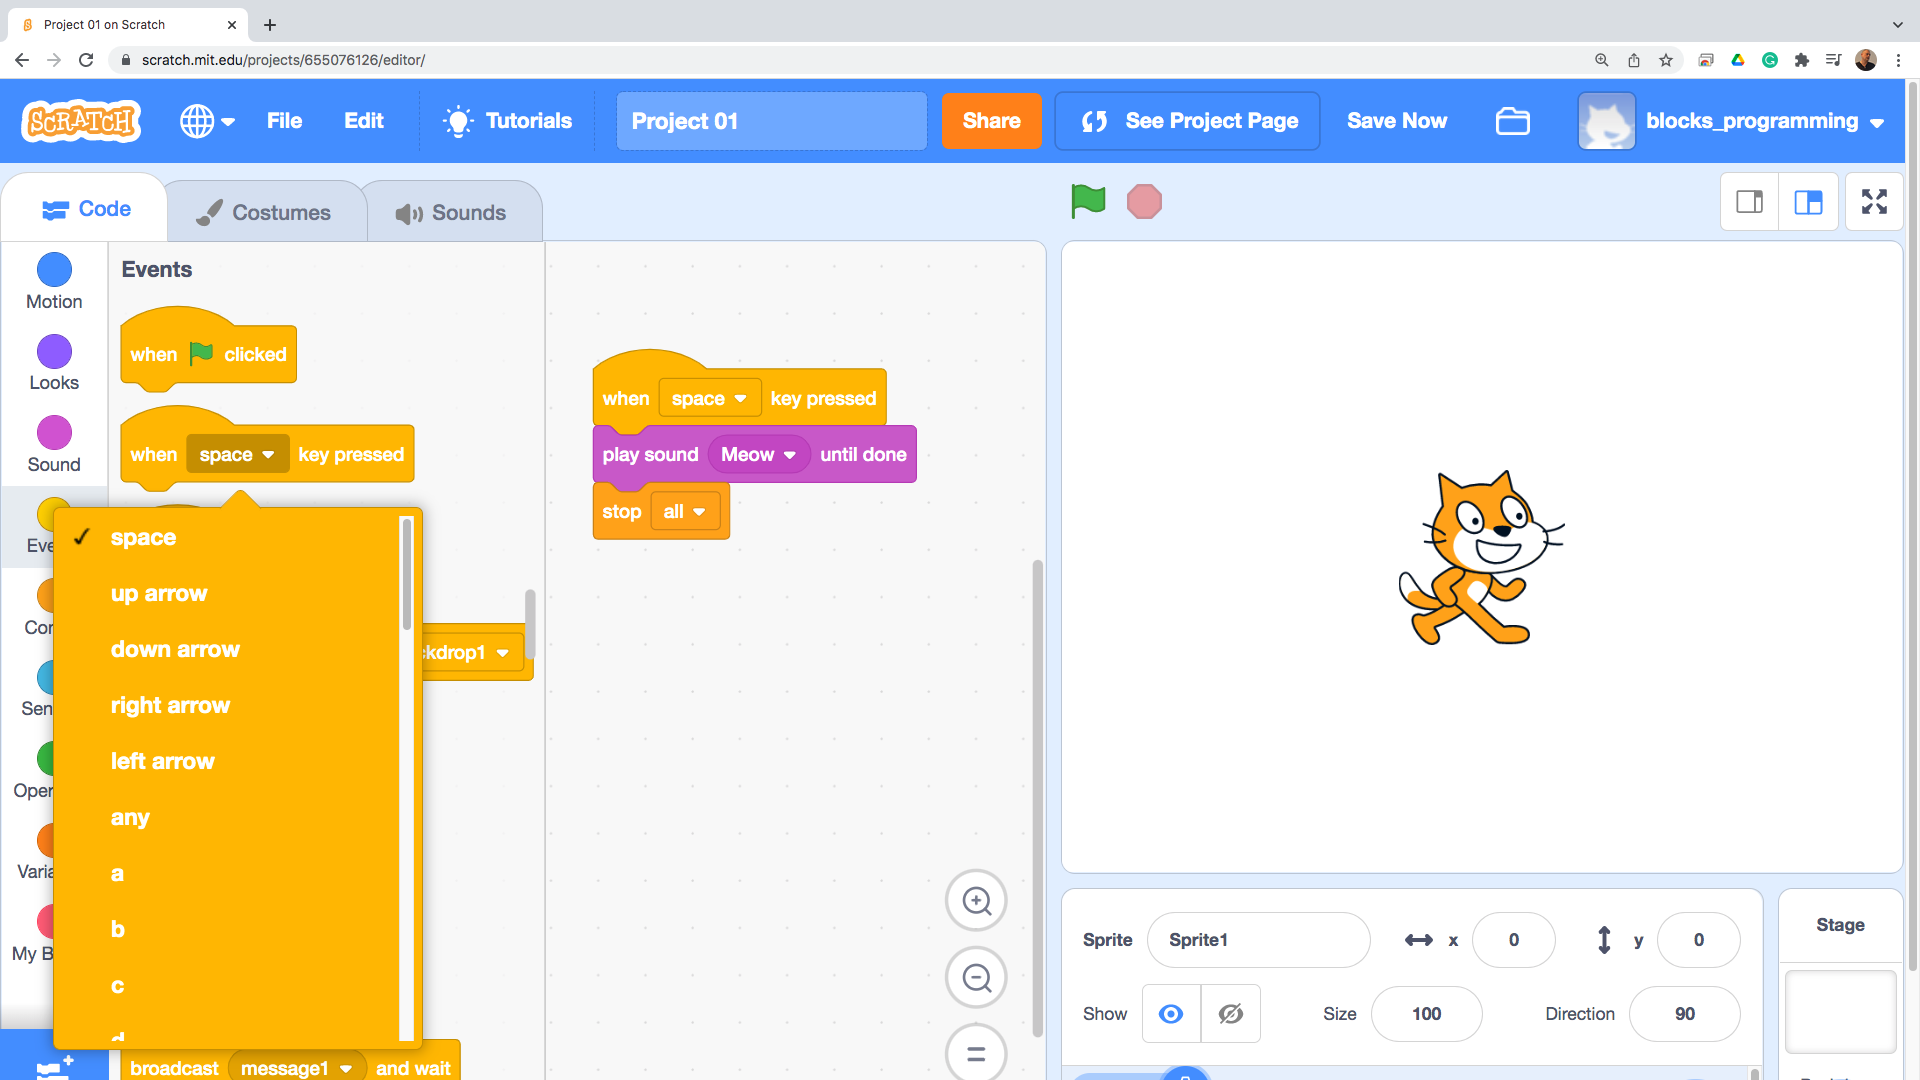
\includegraphics[width=1.0\linewidth,height=0.5\linewidth]{fig0079.png}
%  \caption{Събитие за натискане на клавиш}
%\label{fig0079}
%\end{figure}
%
%Кликването с мишката върху определен спрайт също може да бъде обработено с помощта на подходящо блокче (Фиг. \ref{fig0080}).
%
%\begin{figure}[H]
%  \centering
%  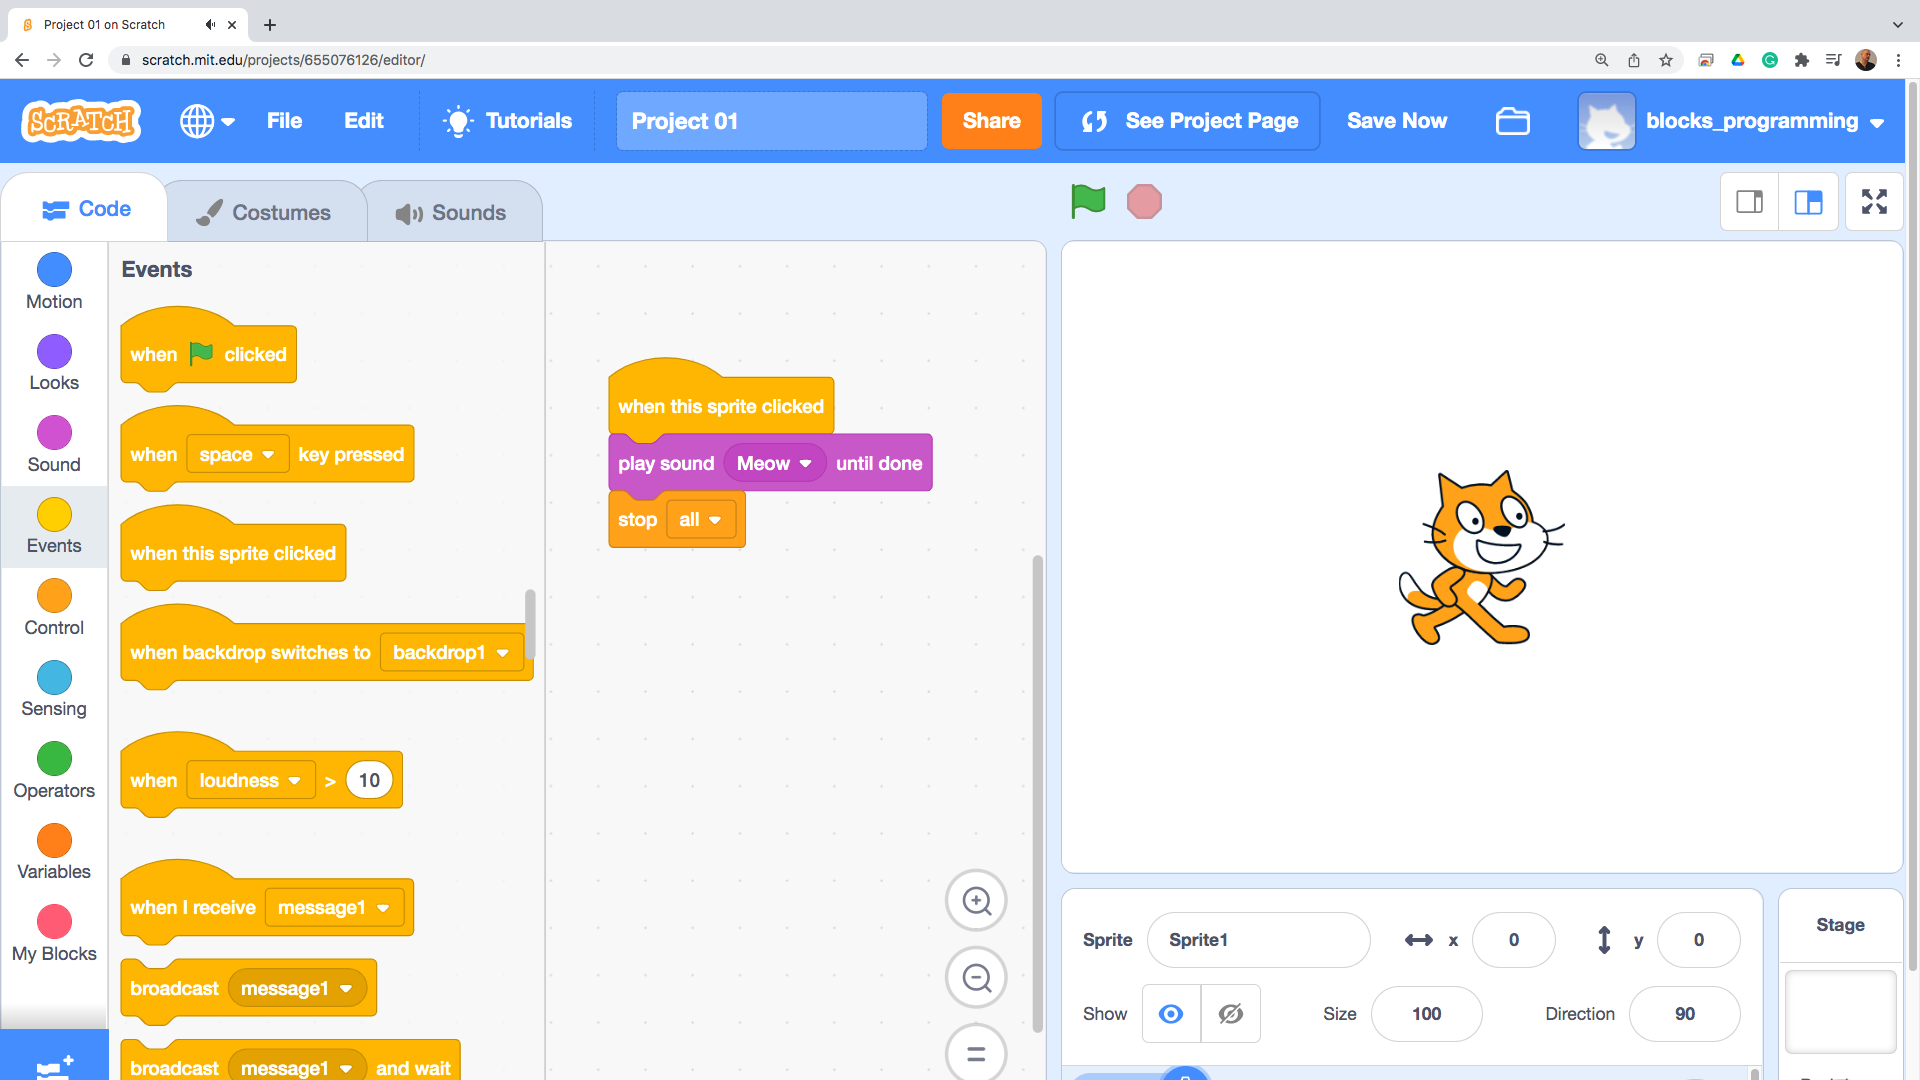
\includegraphics[width=1.0\linewidth,height=0.5\linewidth]{fig0080.png}
%  \caption{Събитие за кликане с мишката}
%\label{fig0080}
%\end{figure}
%
%Смяната на фона също може да предизвика обработване на събитие. За тази цел има предвидено блокче (Фиг. \ref{fig0081}).
%
%\begin{figure}[H]
%  \centering
%  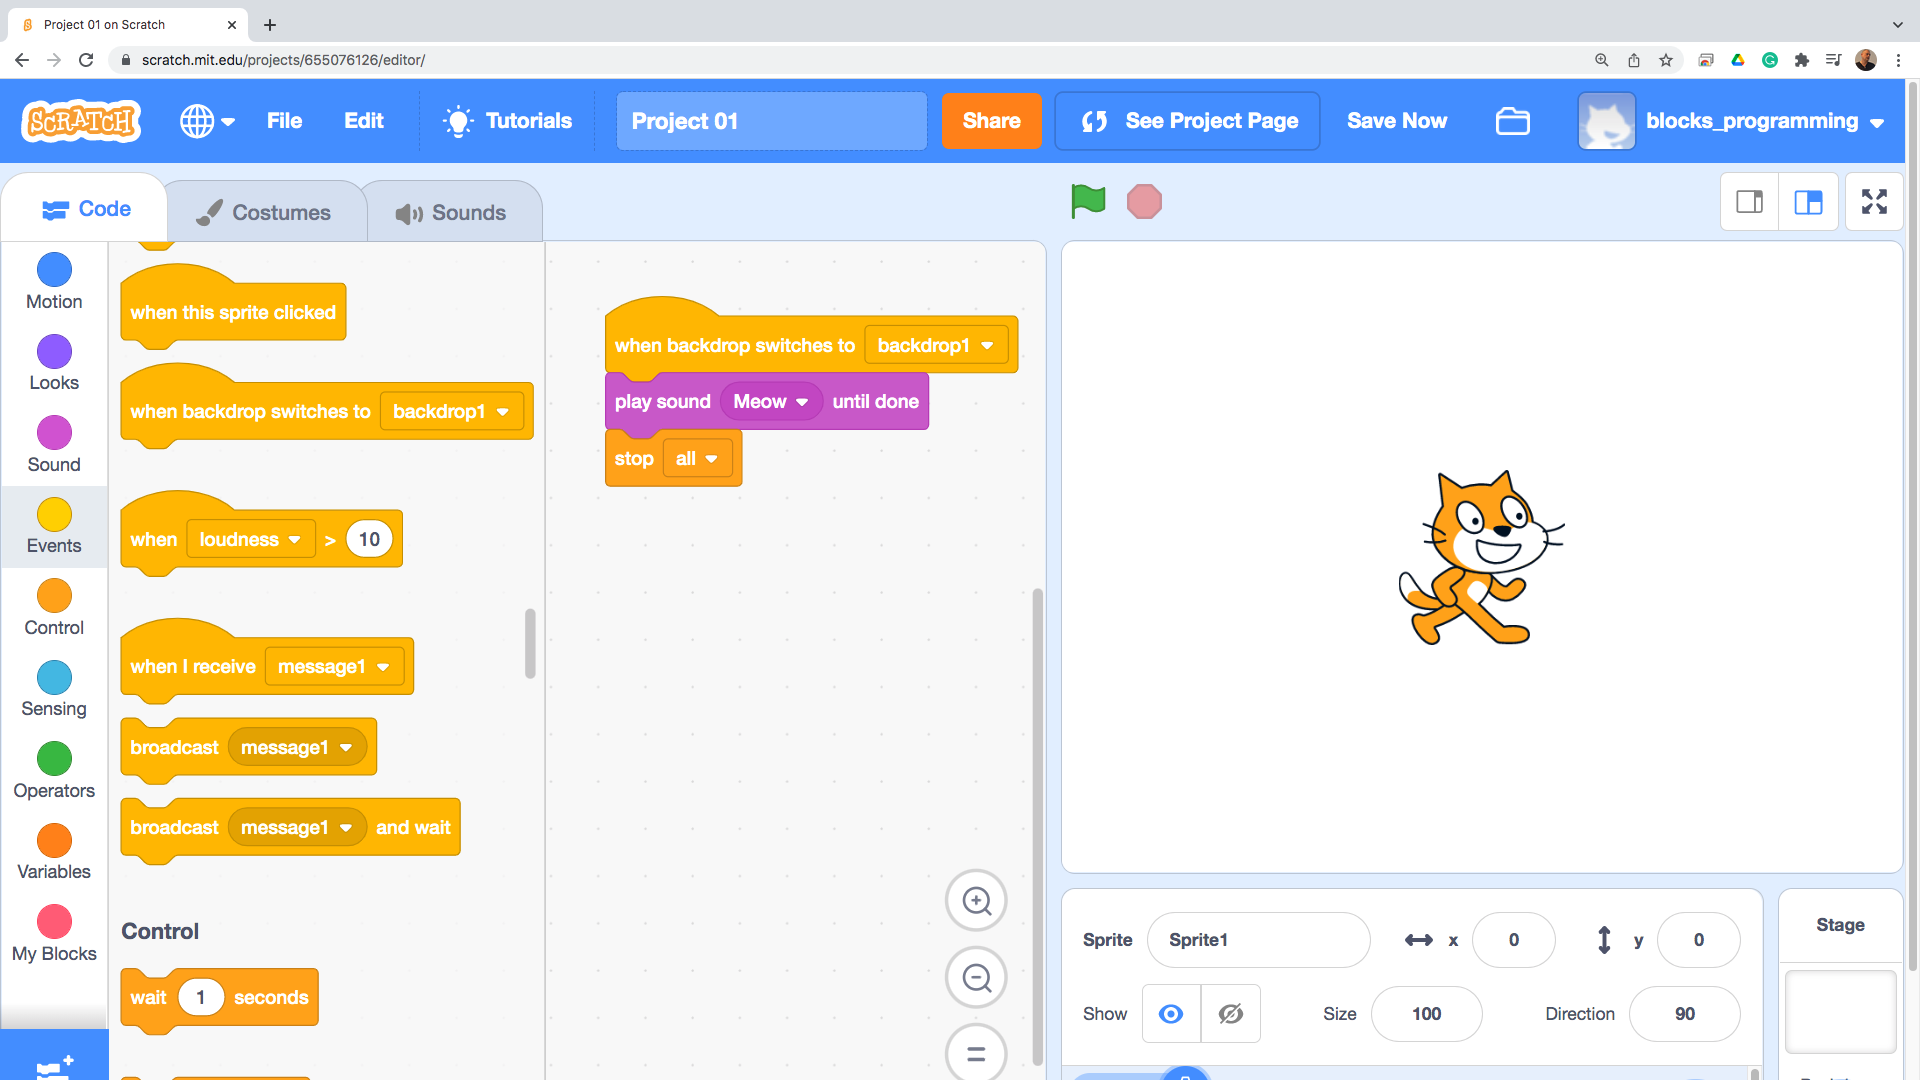
\includegraphics[width=1.0\linewidth,height=0.5\linewidth]{fig0081.png}
%  \caption{Събитие за смяна на фона}
%\label{fig0081}
%\end{figure}
%
%Събитие може да бъде прихванато след изтичане на определено време към таймер или достигане на определено ниво на звук (Фиг. \ref{fig0082}).
%
%\begin{figure}[H]
%  \centering
%  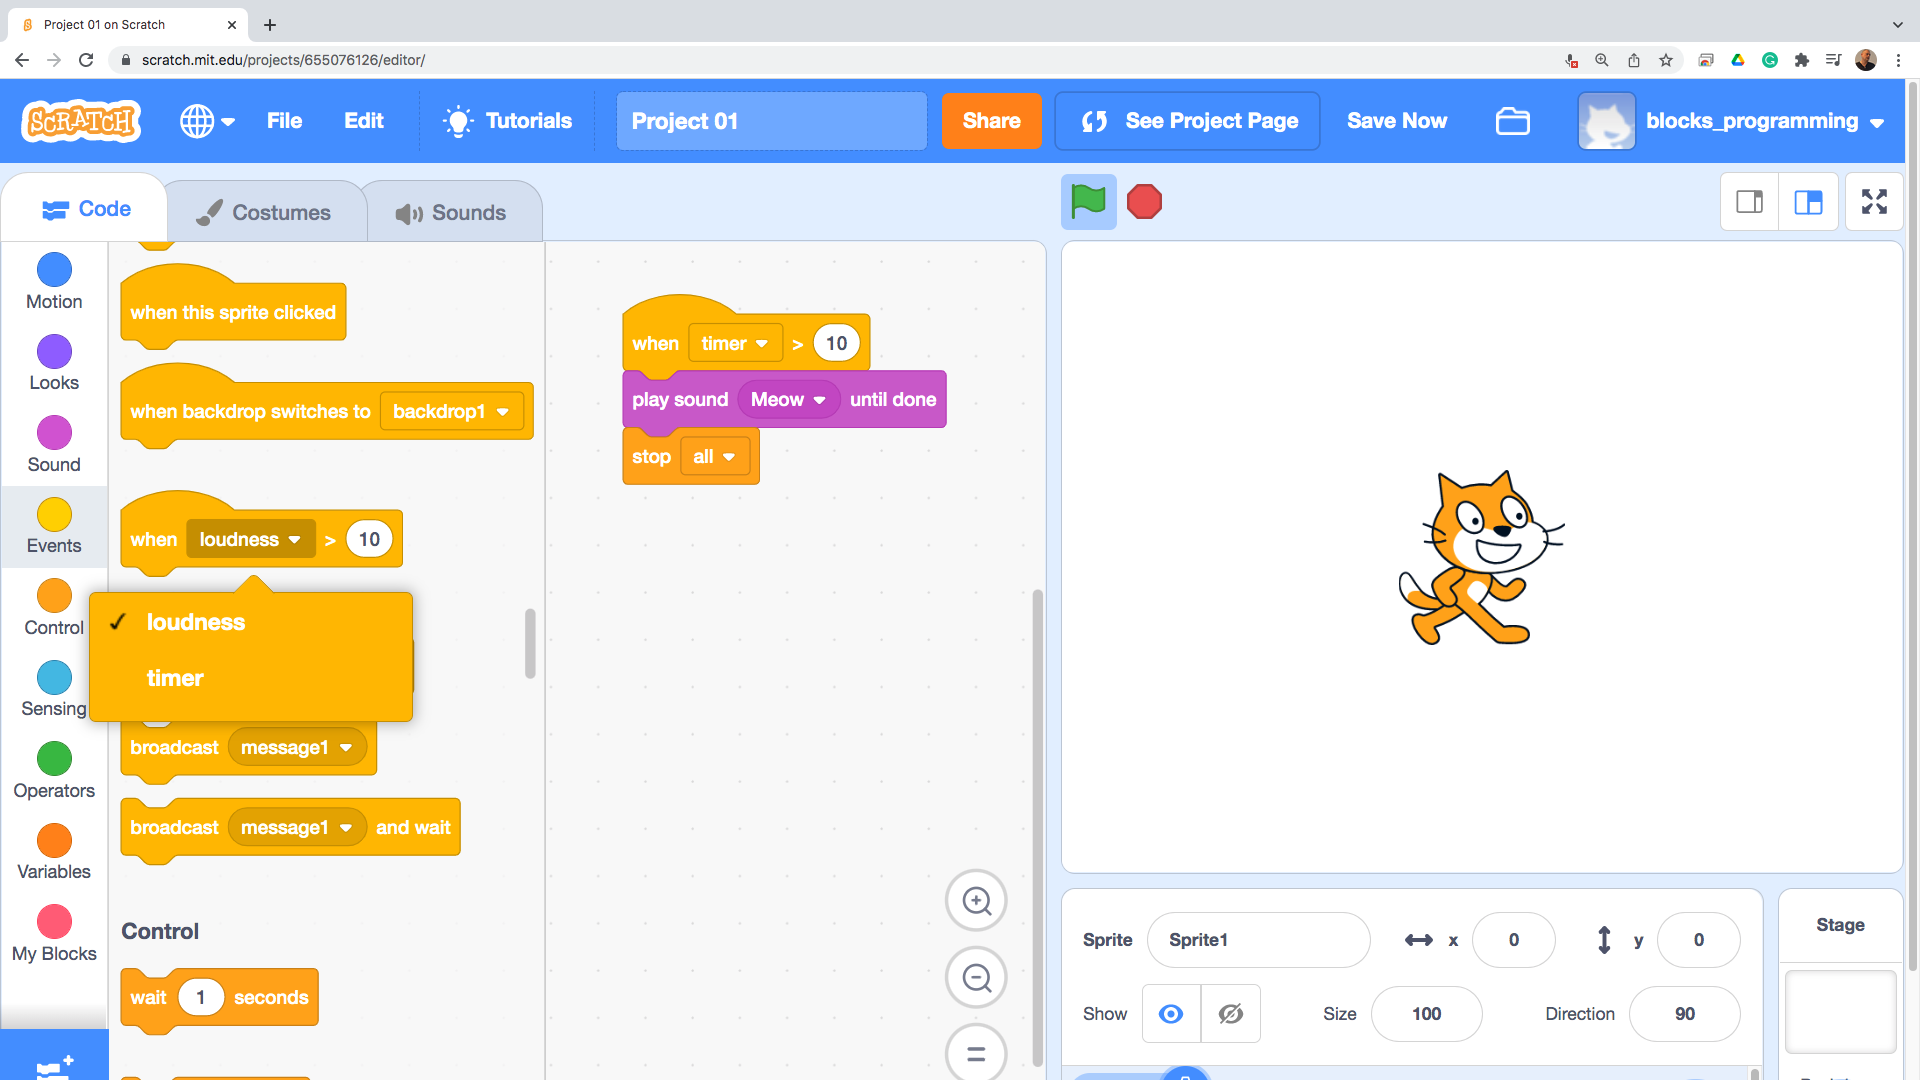
\includegraphics[width=1.0\linewidth,height=0.5\linewidth]{fig0082.png}
%  \caption{Събитие от таймер или звук}
%\label{fig0082}
%\end{figure}
%
%Работата със събития е свързана и с механизъм за предаване/получаване на съобщения. Един блок инструкции може да разпространи предварително дефинирано съобщение, а друг блок инструкции може да се абонира за получаването на точно този вид съобщение (Фиг. \ref{fig0083}).
%
%\begin{figure}[H]
%  \centering
%  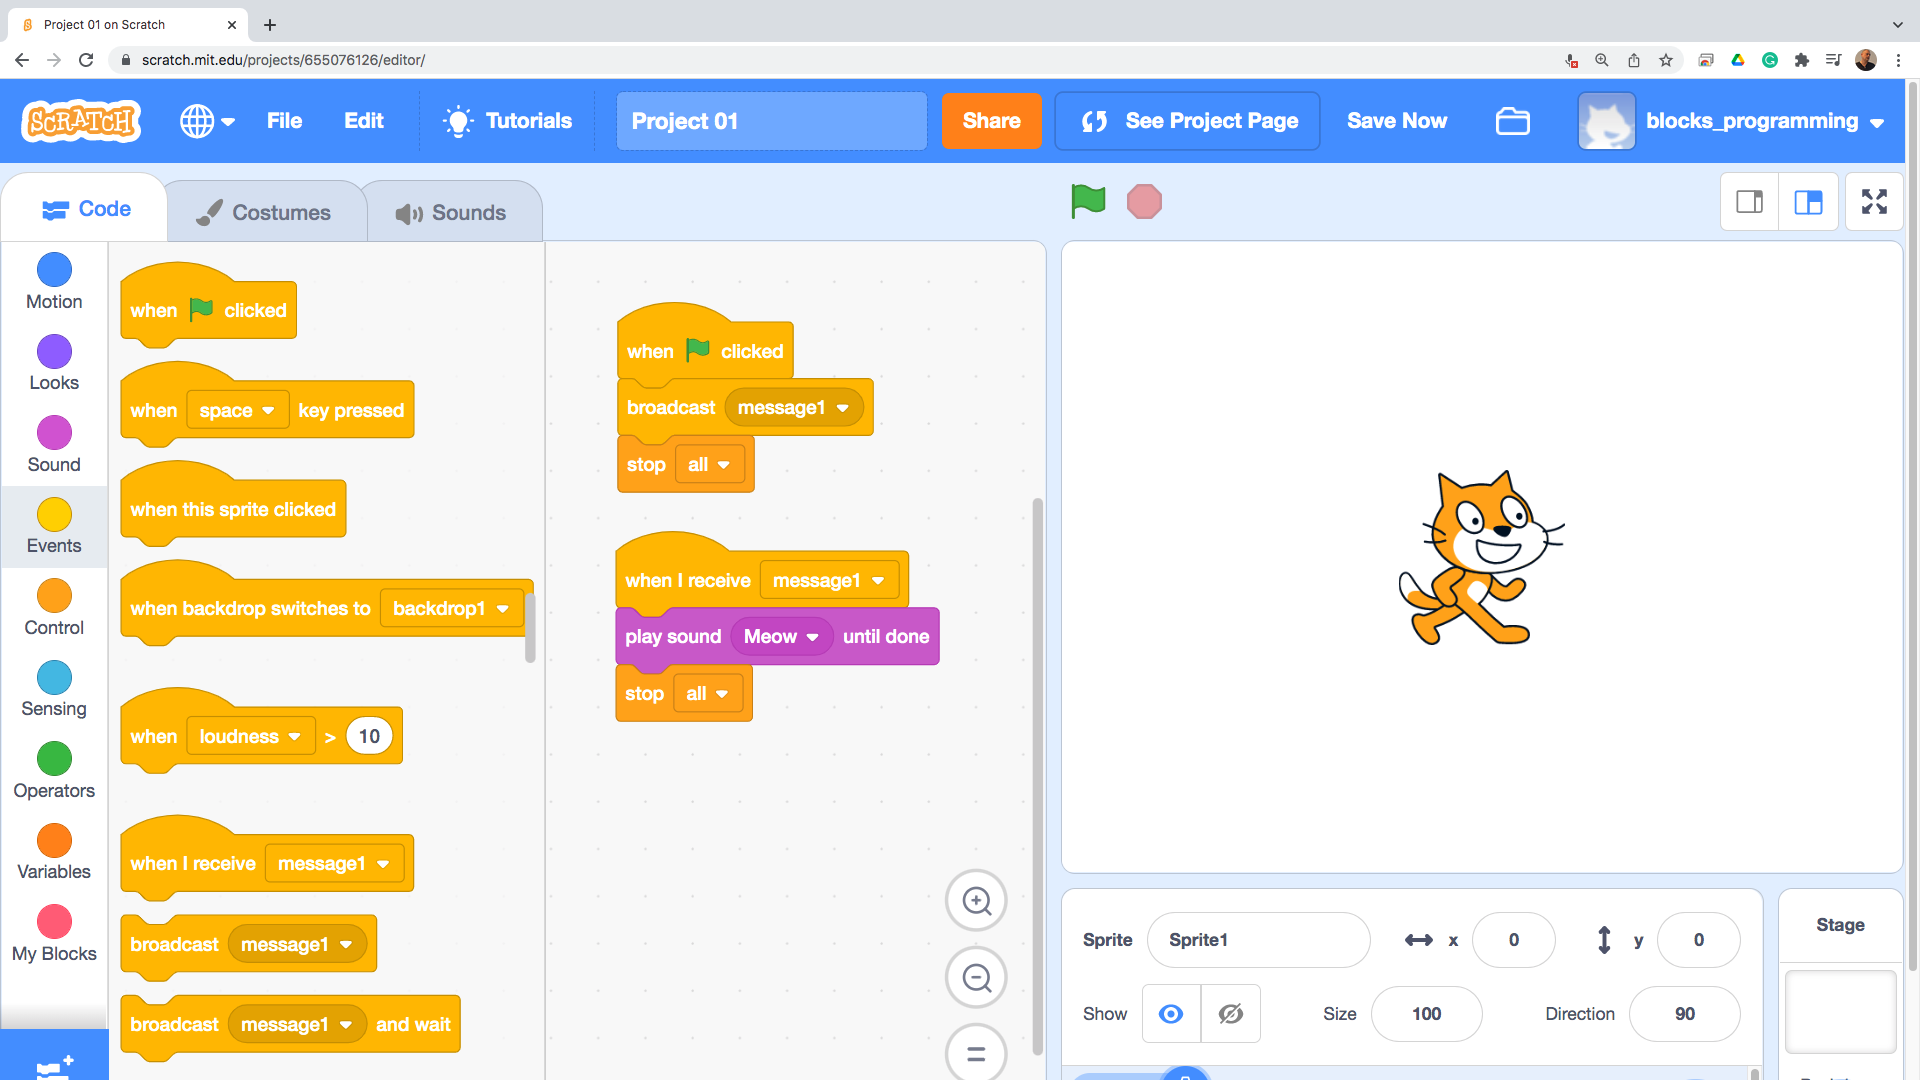
\includegraphics[width=1.0\linewidth,height=0.5\linewidth]{fig0083.png}
%  \caption{Разпространяване и получаване на съобщения}
%\label{fig0083}
%\end{figure}
%
%Тъй като работата с механизма за съобщения може да изисква синхронизация, то има отделно блокче, което разпространява съобщението и изчаква извършването на действията от прихващането му (Фиг. \ref{fig0084}). Програмистът може да създава различни съобщения, които да бъдат изпращани в различни ситуации. 
%
%\begin{figure}[H]
%  \centering
%  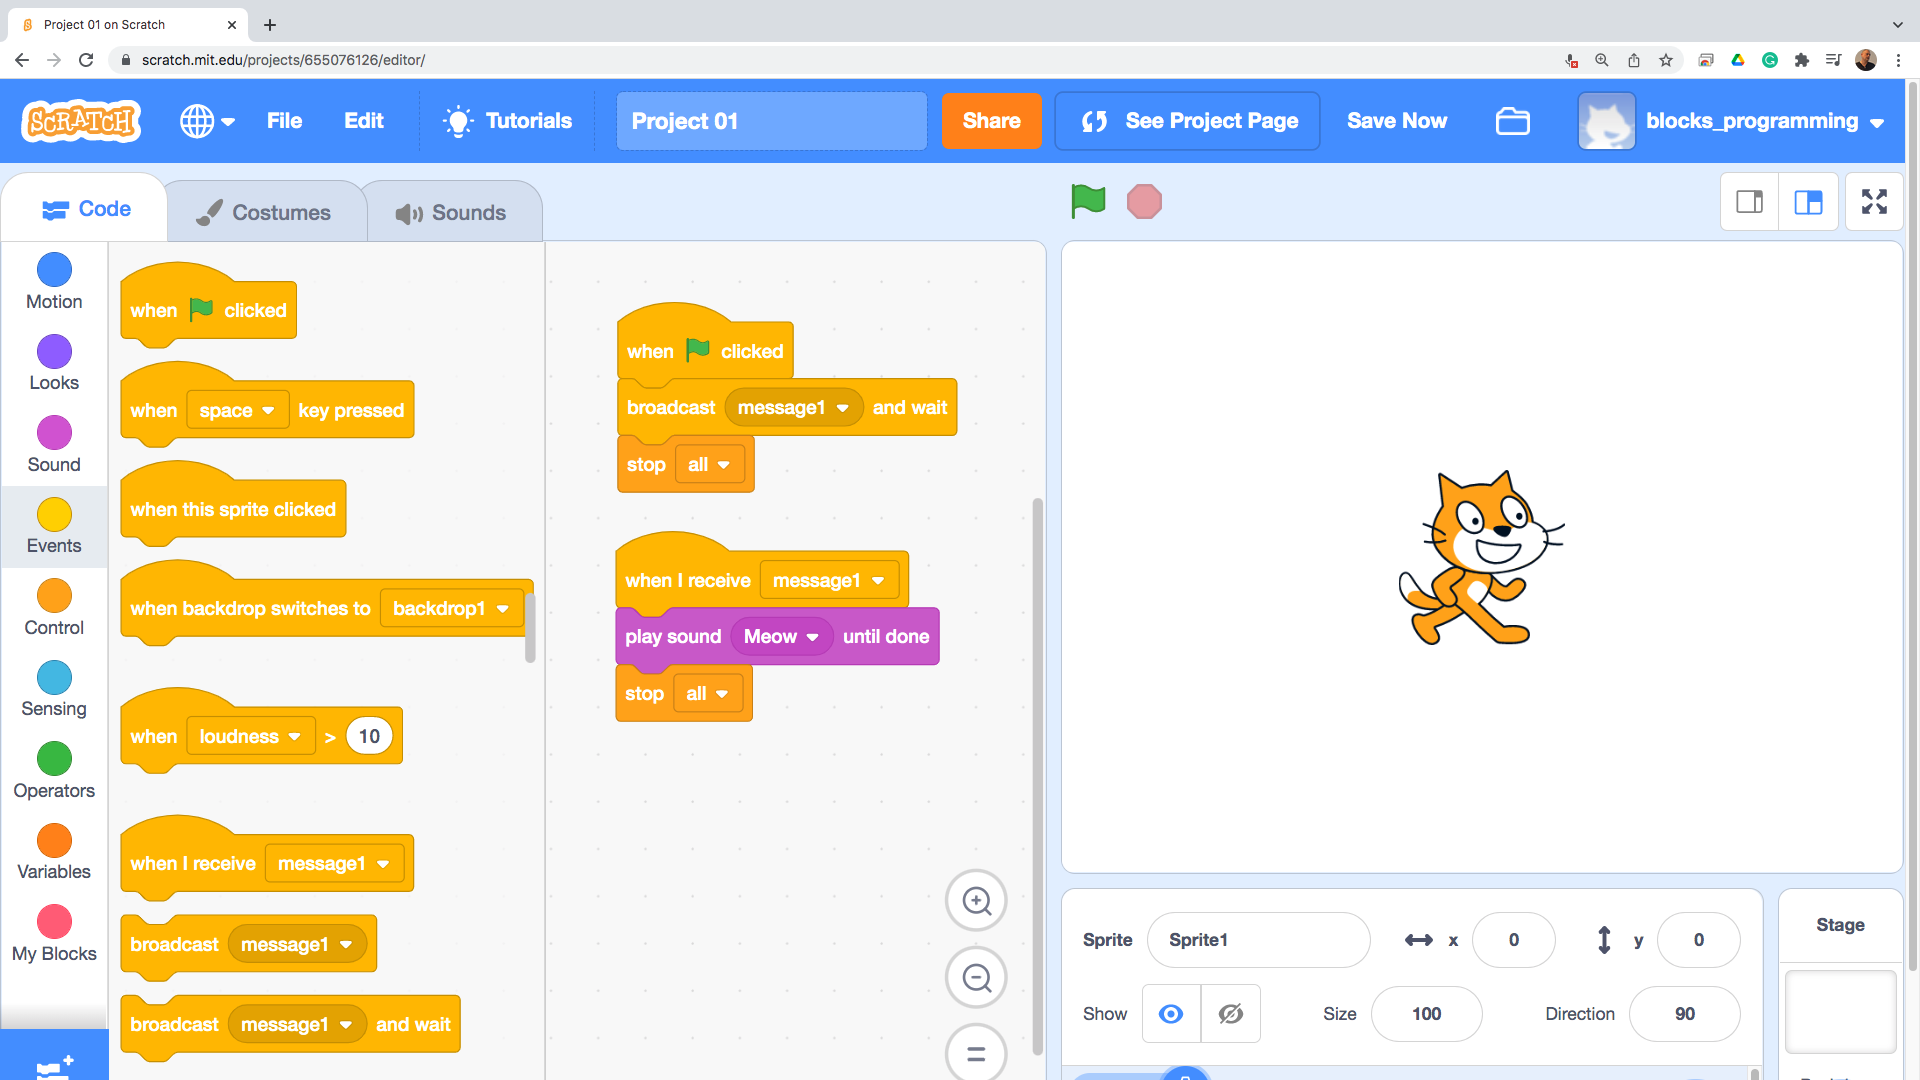
\includegraphics[width=1.0\linewidth,height=0.5\linewidth]{fig0084.png}
%  \caption{Разпространяване на съобщение с изчакване}
%\label{fig0084}
%\end{figure}
%
%Най-важните, а и най-полезните блокчета са организирани в групата на тъмно оранжевите. Това са блокчета, които определят по коя пътека на изпълнение ще се поеме, спрямо възможните избори за изпълнение на инструкции. Когато желанието е определено действие да се изпълни многократно, при зададен брой повторения, за тази цел има конкретно блокче (Фиг. \ref{fig0085}). В програмирането, многократните повторения се осъществяват с помощта на конструкции за цикъл, какъвто е случаят и с това блокче за повторения.
%
%\begin{figure}[H]
%  \centering
%  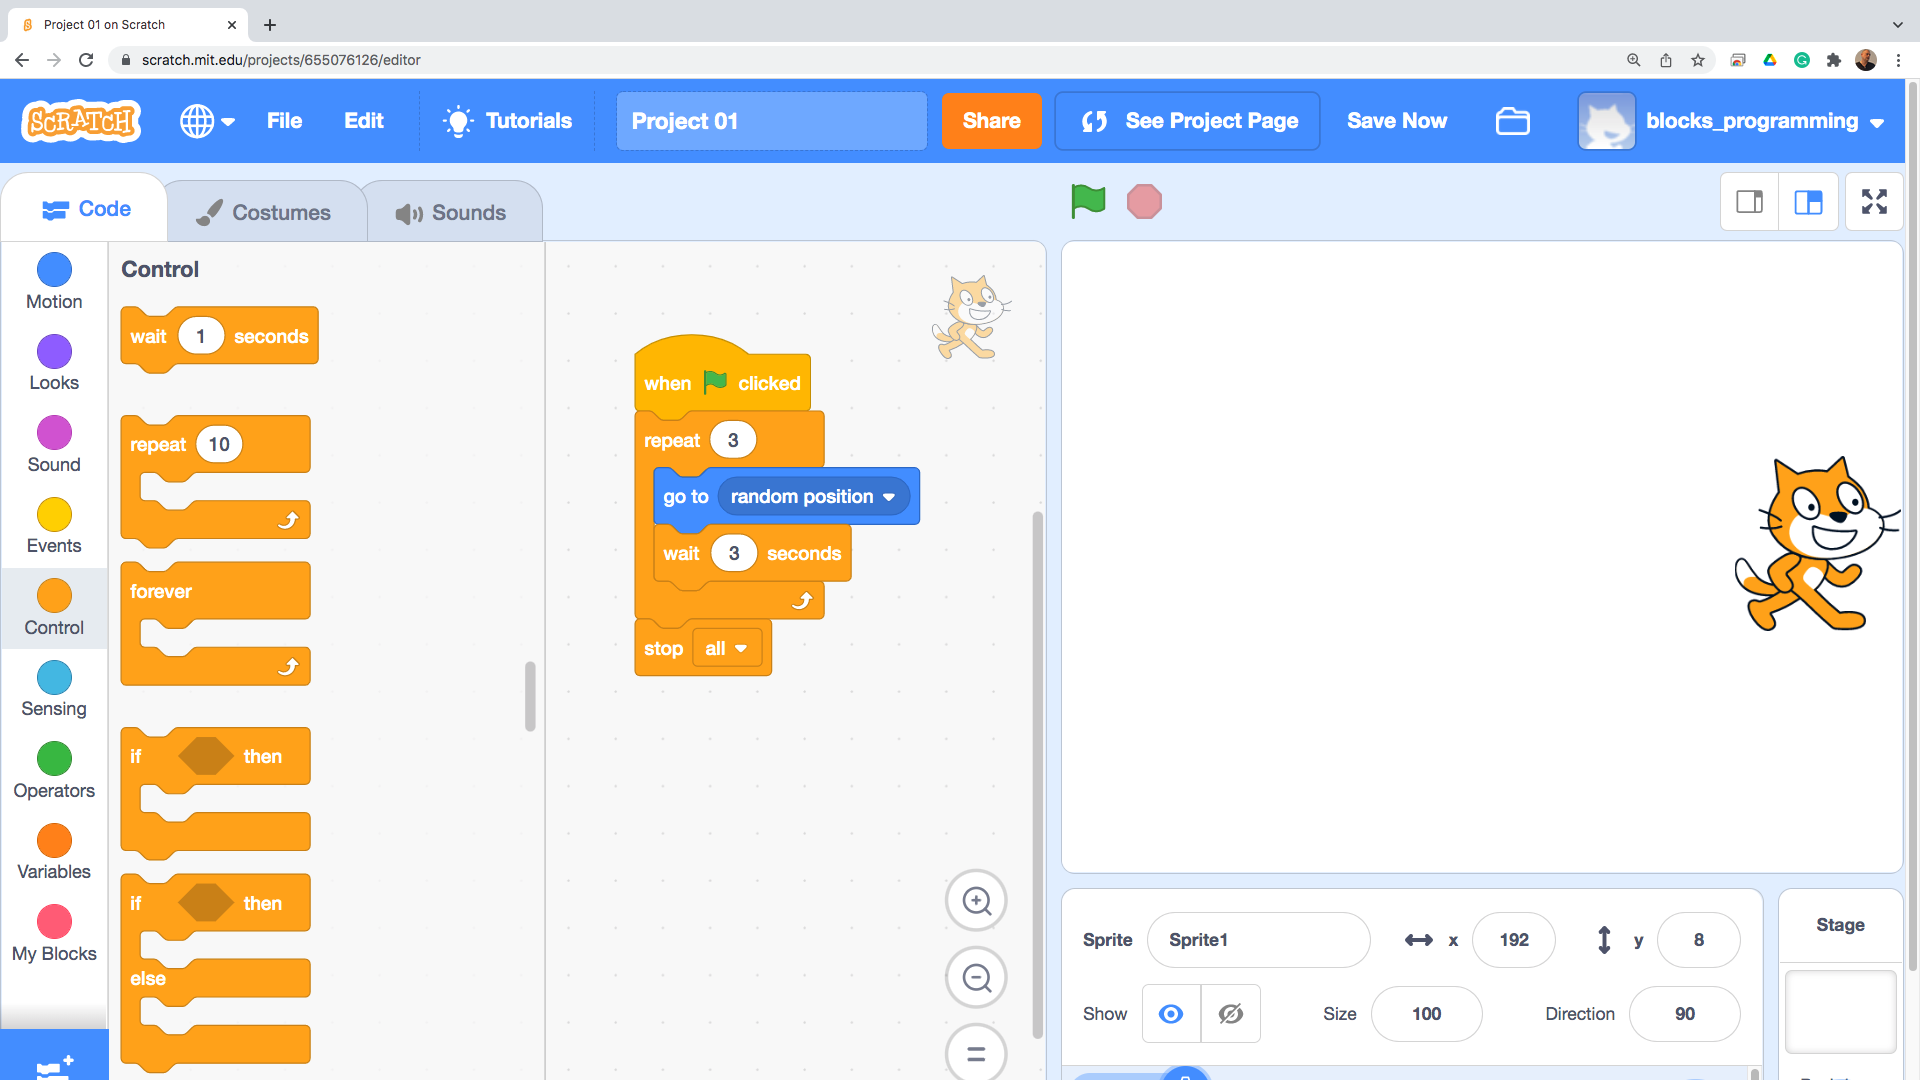
\includegraphics[width=1.0\linewidth,height=0.5\linewidth]{fig0085.png}
%  \caption{Фиксиран брой повторения}
%\label{fig0085}
%\end{figure}
%
%Думичката repeat от английски означава повтори. Числото в блокчето определя колко на брой повторения да бъдат изпълнени, а в слота на блочето се поставят инструкциите, които да бъдат повтаряни. В този пример, котето се премества на случайно избрани координати, след което следва изчакване от предварително определен брой секунди. В много редки ситуации има нужда от безкрайно повтарящ се цикъл, за което е предвидено отделно блокче (Фиг. \ref{fig0086}).
%
%\begin{figure}[H]
%  \centering
%  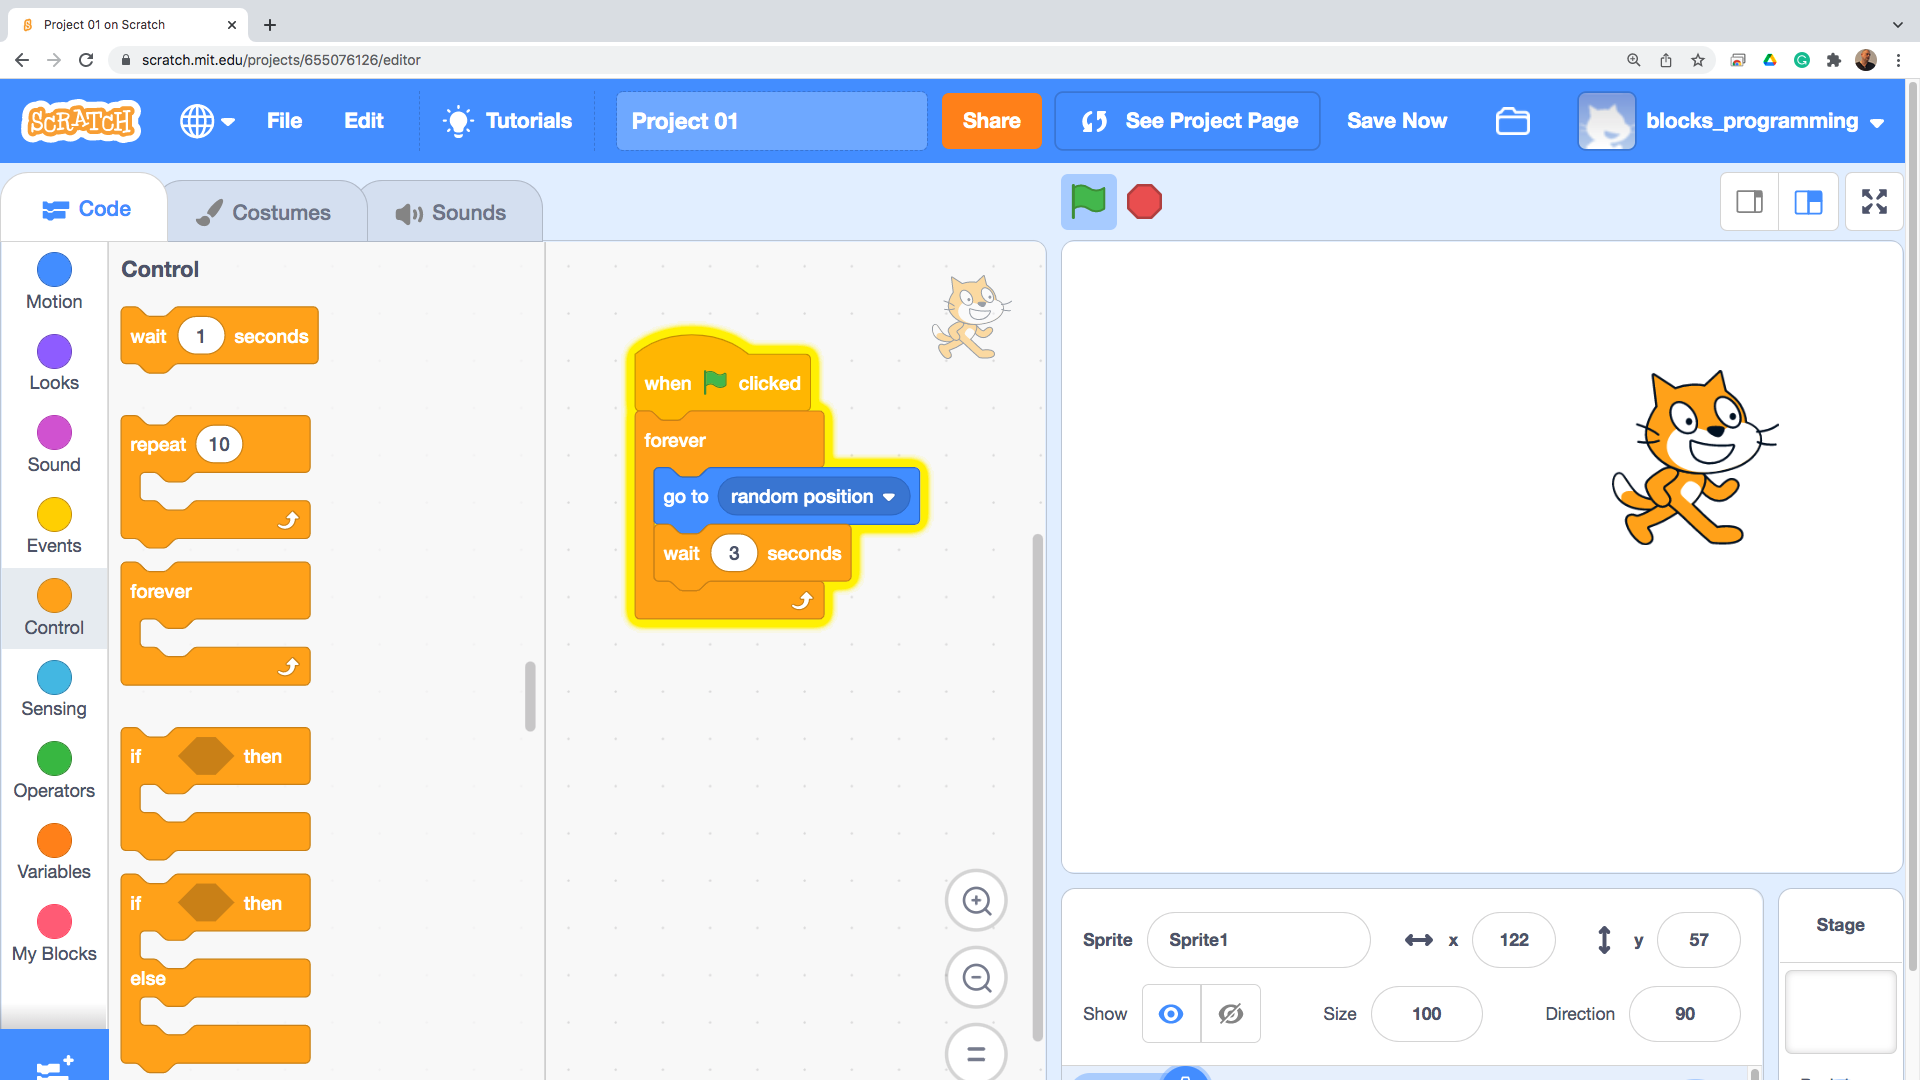
\includegraphics[width=1.0\linewidth,height=0.5\linewidth]{fig0086.png}
%  \caption{Безкрайни повторения}
%\label{fig0086}
%\end{figure}
%
%Следващото блокче е едно от най-важните блокчета в програмирането. То се нарича блокче за изпълнение при условие (Фиг. \ref{fig0087}) или условен преход. Съдържанието на блокчето се изпълнява само, ако условието в заглавната му част се изпълнява.
%
%\begin{figure}[H]
%  \centering
%  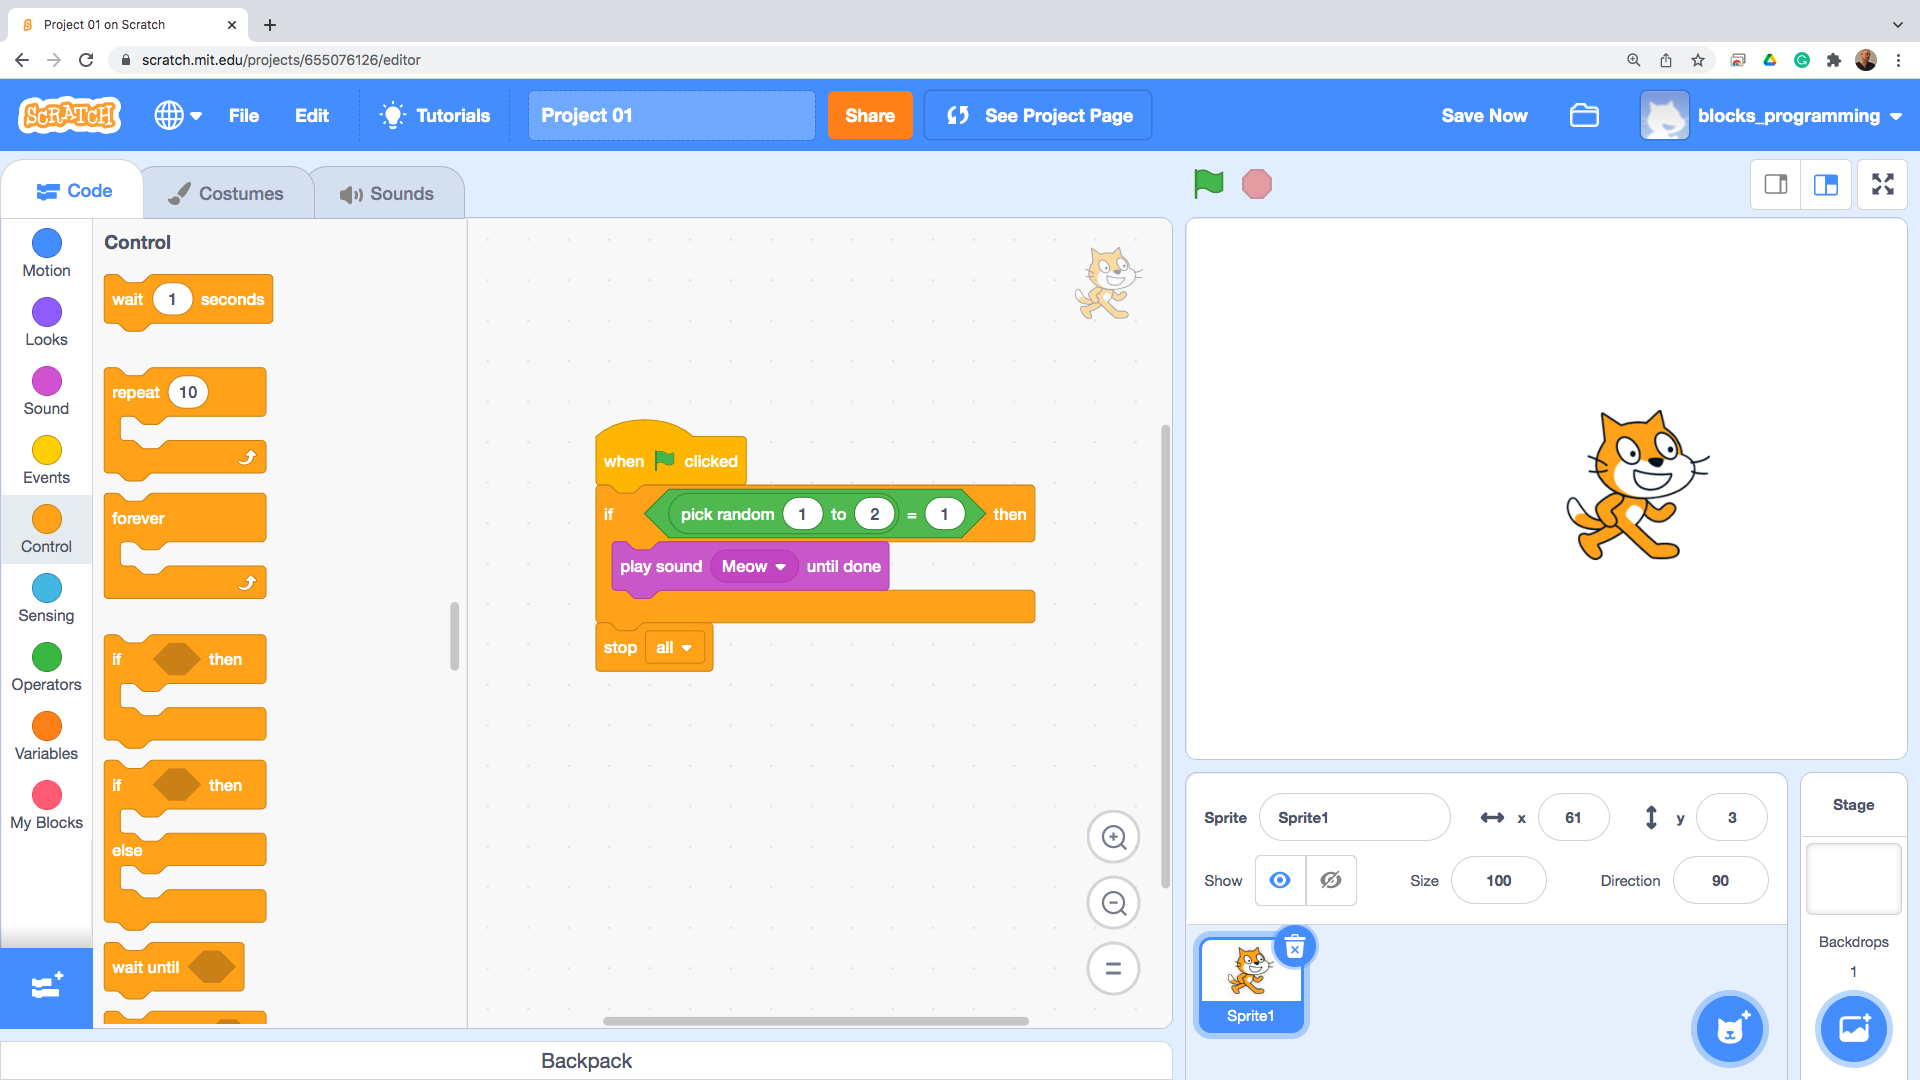
\includegraphics[width=1.0\linewidth,height=0.5\linewidth]{fig0087.png}
%  \caption{Изпълнение при условие}
%\label{fig0087}
%\end{figure}
%
%Това тъмно оранжево блокче не може да се използва само. То винаги е в съчетание с поне едно зелено блокче, а понякога и с две, както е в настоящия пример. Част от зелените блокчета са неправилни шестоъгълници и са направени така, че да пасват в заглавната част на някои от тъмно оранжевите блокчета. Самото шестоъгълно блокче има овален слот в който се поместват някои от зелените овални блокчета. В примера е избрано зелено блокче, което изисква равенство към конкретно число, а за овалното блокче се ползва генератор на случайни числа, според предварително зададен интервал. Ако условието в заглавната част на блокчето за условен преход не бъде изпълнено, то тялото се пропуска и се преминава към следващите инструкции, след блочкето. Блокчето за условен преход има и вариант в който се предвиждат слотове за изпълнение и на двете възможности – вярно условие или невярно условие (Фиг. \ref{fig0088}). Ако условието е изпълнено, се изпълнява първият блок с инструкции. Ако условието не е изпълнено, се изпълнява вторият блок с инструкции.
%
%\begin{figure}[H]
%  \centering
%  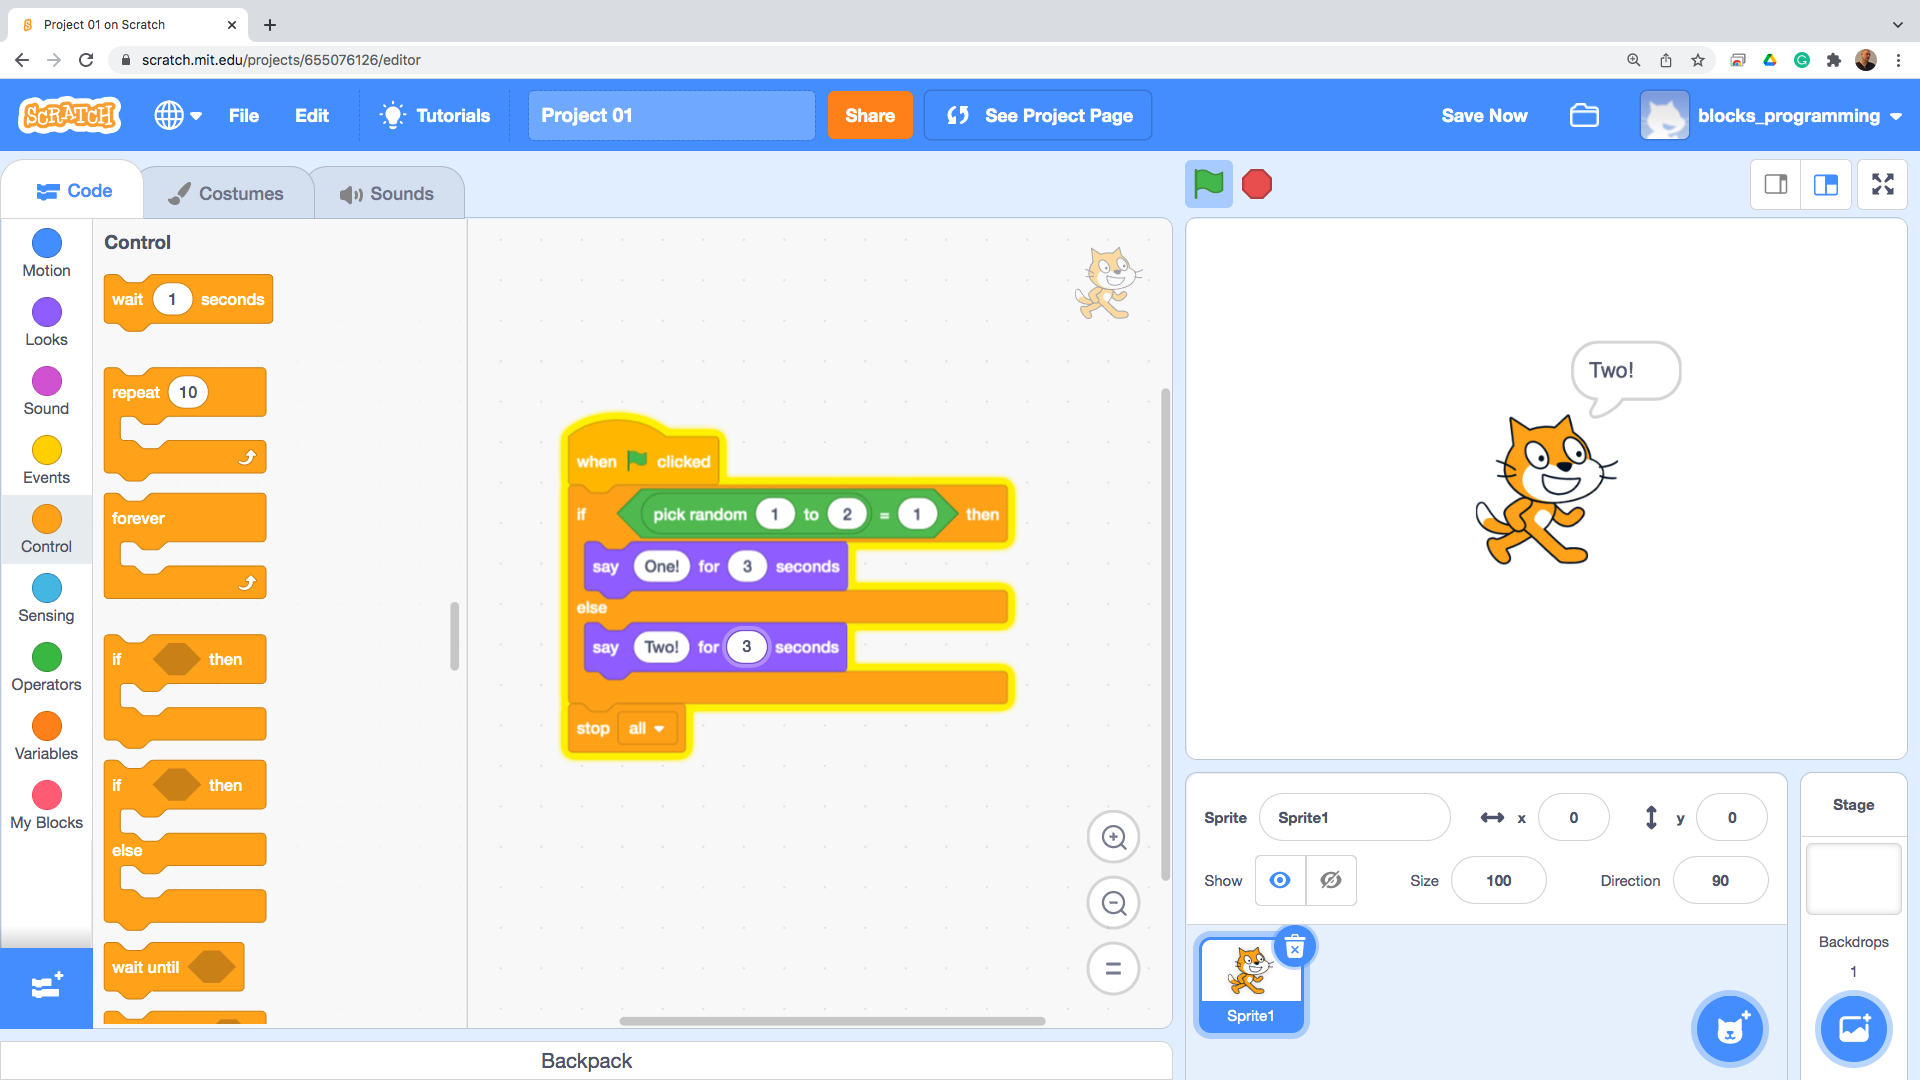
\includegraphics[width=1.0\linewidth,height=0.5\linewidth]{fig0088.png}
%  \caption{Изпълнение при условие с алтернатива}
%\label{fig0088}
%\end{figure}
%
%Следващото интересно блокче прави изчакване докато се случи определено събитие. В случая, събитието е спрайтът да бъде докоснат с мишката (Фиг. \ref{fig0089}). Случи ли се това докосване, изпълнението на програмата продължава към следващото блокче. Какво събитие се очаква е определено с допълнително блокче (светло синьо), което има формата на неправилен шестоъгълник.
%
%\begin{figure}[H]
%  \centering
%  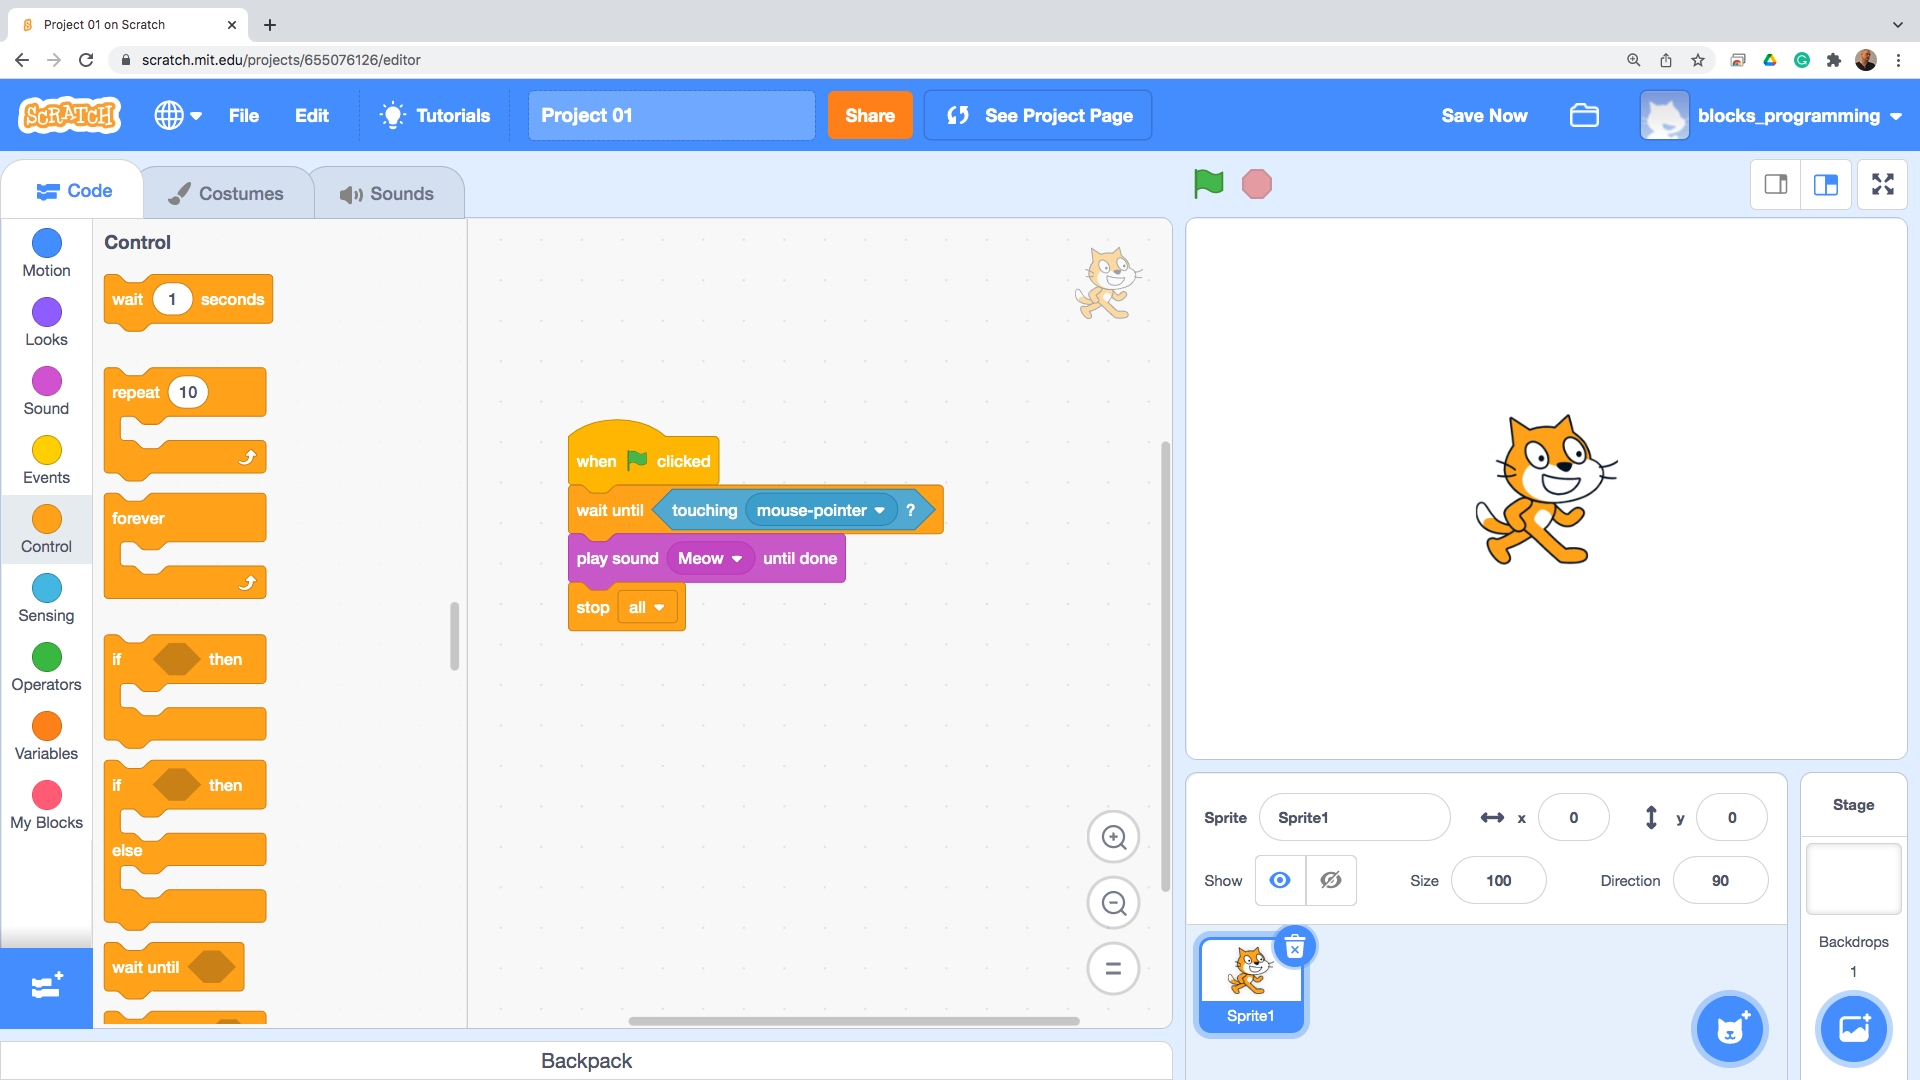
\includegraphics[width=1.0\linewidth,height=0.5\linewidth]{fig0089.png}
%  \caption{Изчакване на условие}
%\label{fig0089}
%\end{figure}
%
%Последните три блокчета в групата на тъмно оранжевите трябва да се демонстрират заедно (Фиг. \ref{fig0090}). Първото блокче задава нова верига от инструкции, когато определен спрай бъде клониран (копие на оригиналния спрайт). Второто блокче служи за клониране на текущия спрайт. А третото блокче служи за изтриване на текущия спрайт. 
%
%\begin{figure}[H]
%  \centering
%  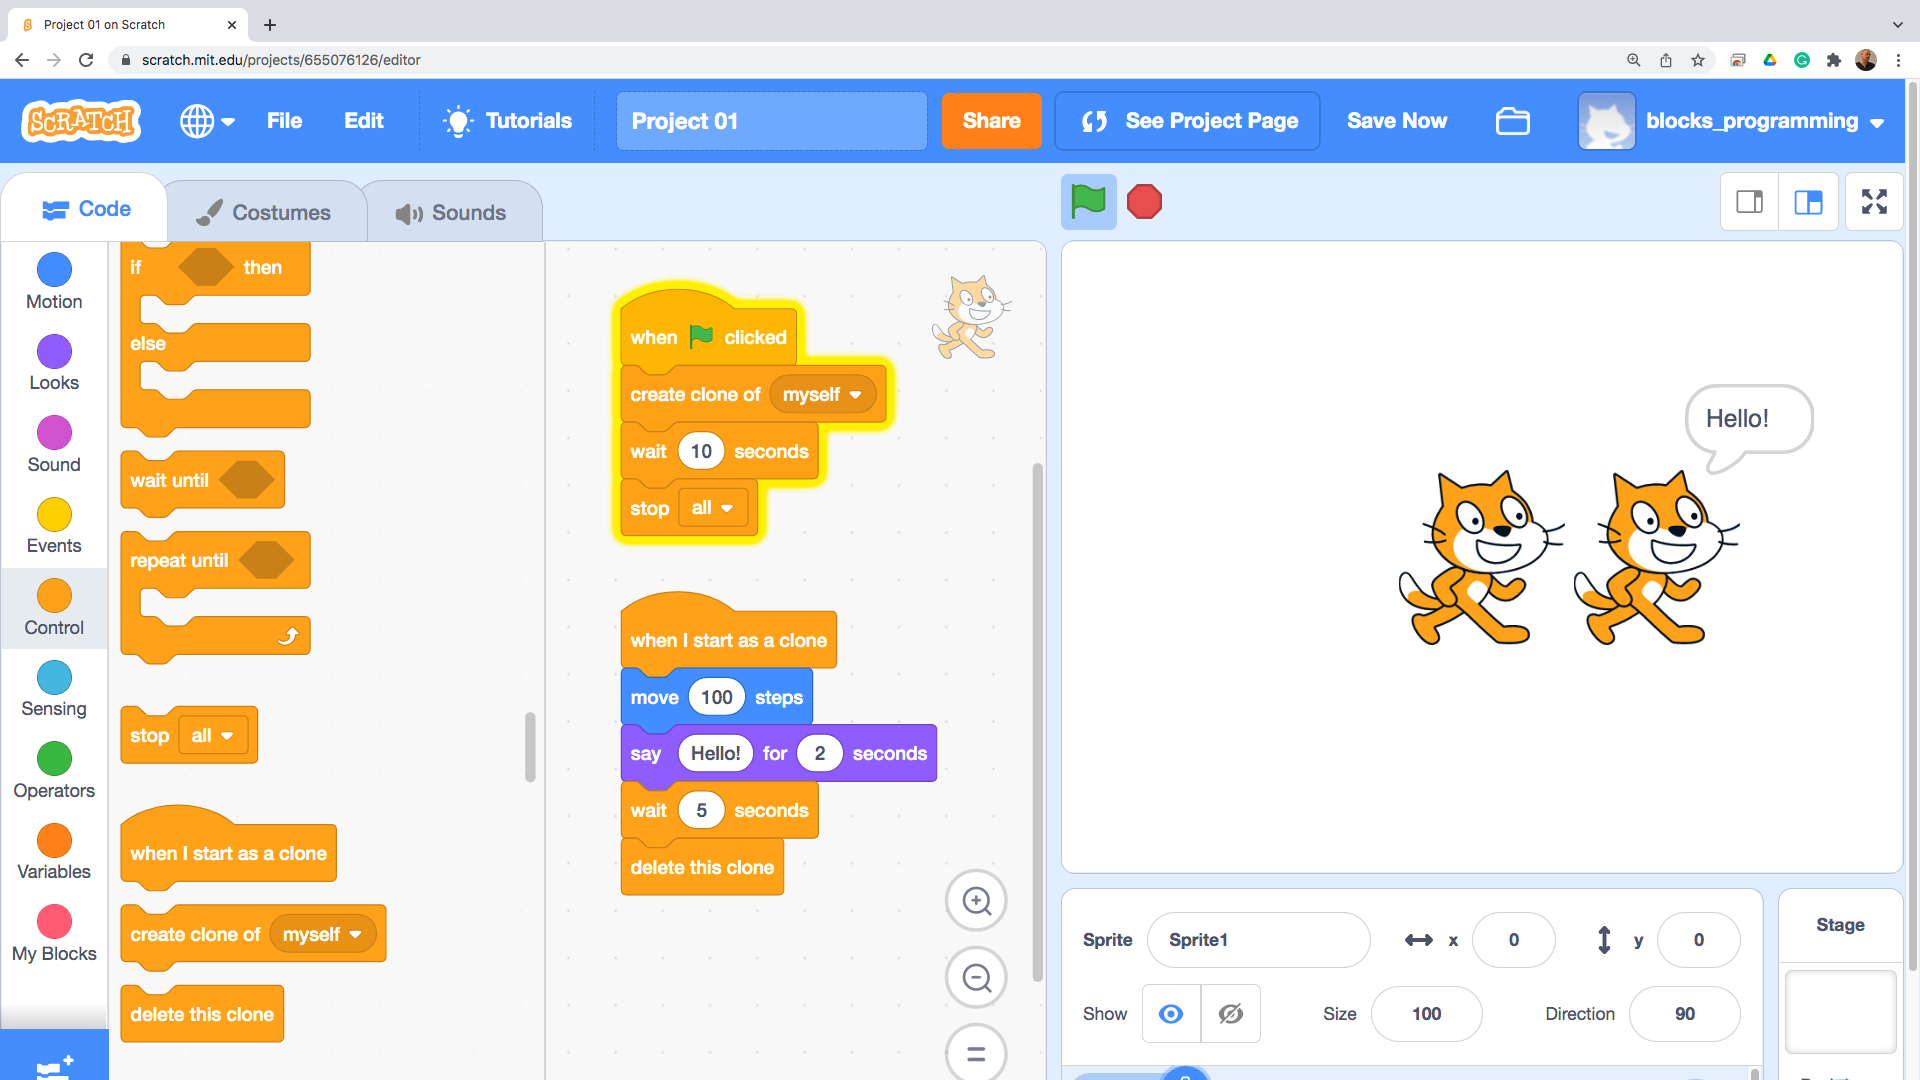
\includegraphics[width=1.0\linewidth,height=0.5\linewidth]{fig0090.png}
%  \caption{Клониране на спрайтове}
%\label{fig0090}
%\end{figure}
%
%Групата на светлосините блокчета е посветена на взаимодействия, отнасящите се до спрайта. Второто блокче в групата е предвидено за изпълняване на условие, когато спрайтът докосне конкретен цвят. Блокчето е с шестоъгълна форма, което подсказва, че е предназначено за вграждане. За да се демонстрира работата на това блокче, ще се завърти един цикъл, който ще премества котето на случайни координати и ще изчаква малък интервал от време, преди следващото преместване (Фиг. \ref{fig0091}). 
%
%\begin{figure}[H]
%  \centering
%  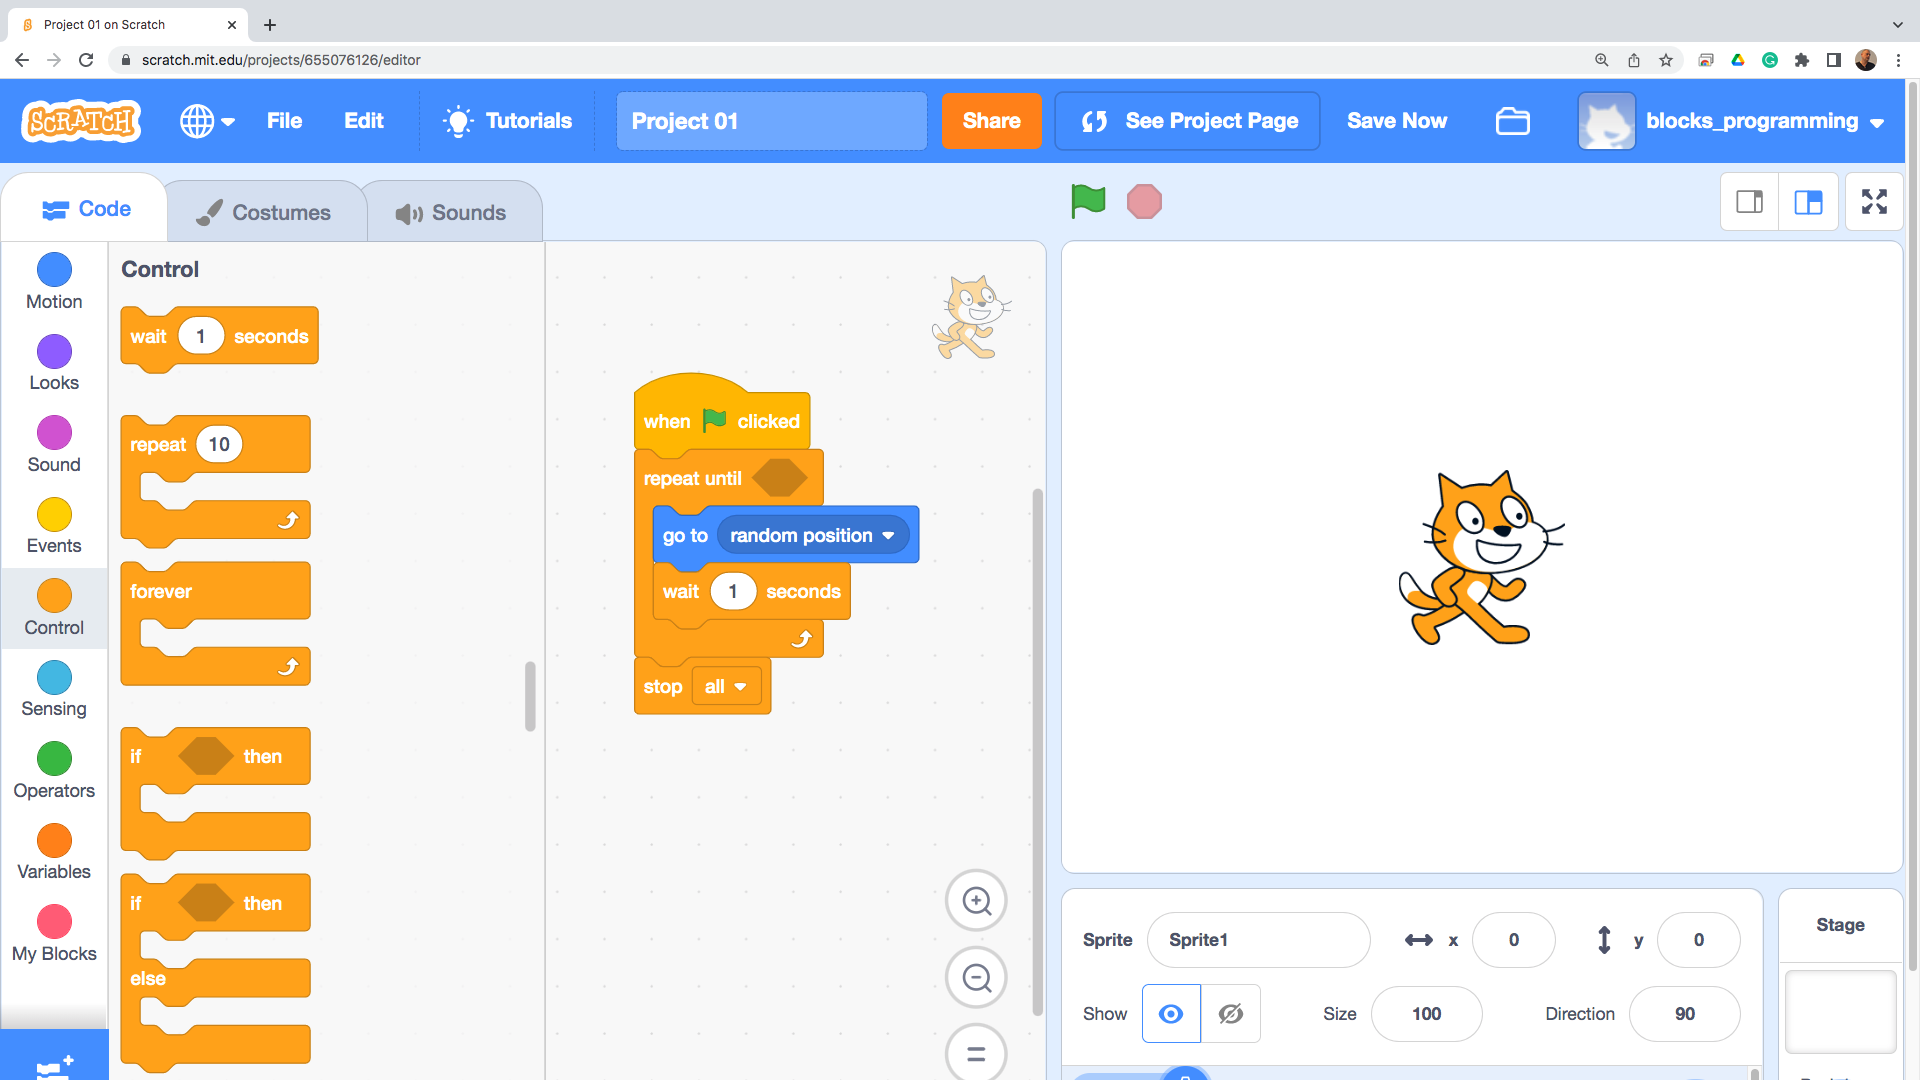
\includegraphics[width=1.0\linewidth,height=0.5\linewidth]{fig0091.png}
%  \caption{Циклично прескачане на случайни координати}
%\label{fig0091}
%\end{figure}
%
%Така направен цикълът ще се върти безкрайно, тъй като не е зададено условие за край. Точно в условието за край мое да се помести блокчето, определящо докосването на цвят. Към сцената ще добавим нов спрайт (Фиг. \ref{fig0092}), на една червена ябълка (Фиг. \ref{fig0093}), която котето трябва да хване. Щом я хване, ще спре да подсказа и ще измяука (Фиг. \ref{fig0094}). 
%
%\begin{figure}[H]
%  \centering
%  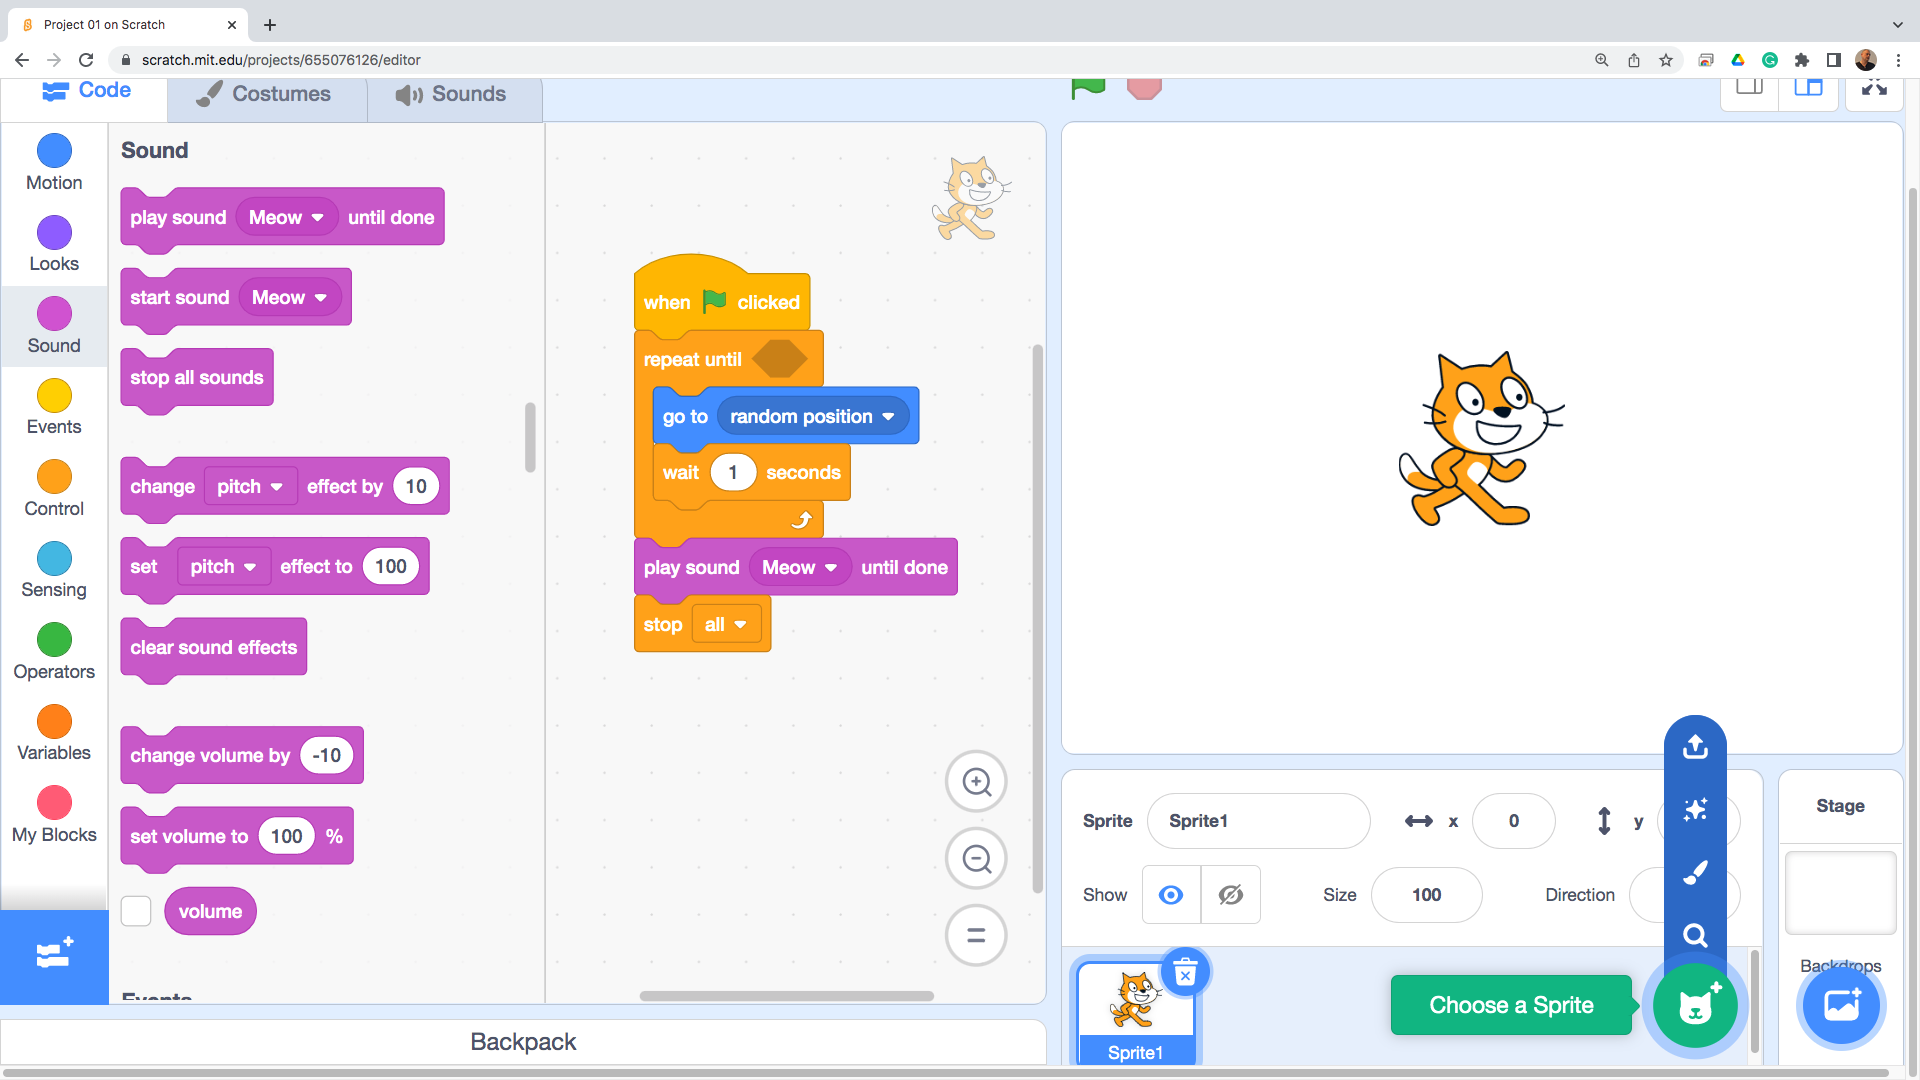
\includegraphics[width=1.0\linewidth,height=0.5\linewidth]{fig0092.png}
%  \caption{Добавяне на спрайт}
%\label{fig0092}
%\end{figure}
%
%\begin{figure}[H]
%  \centering
%  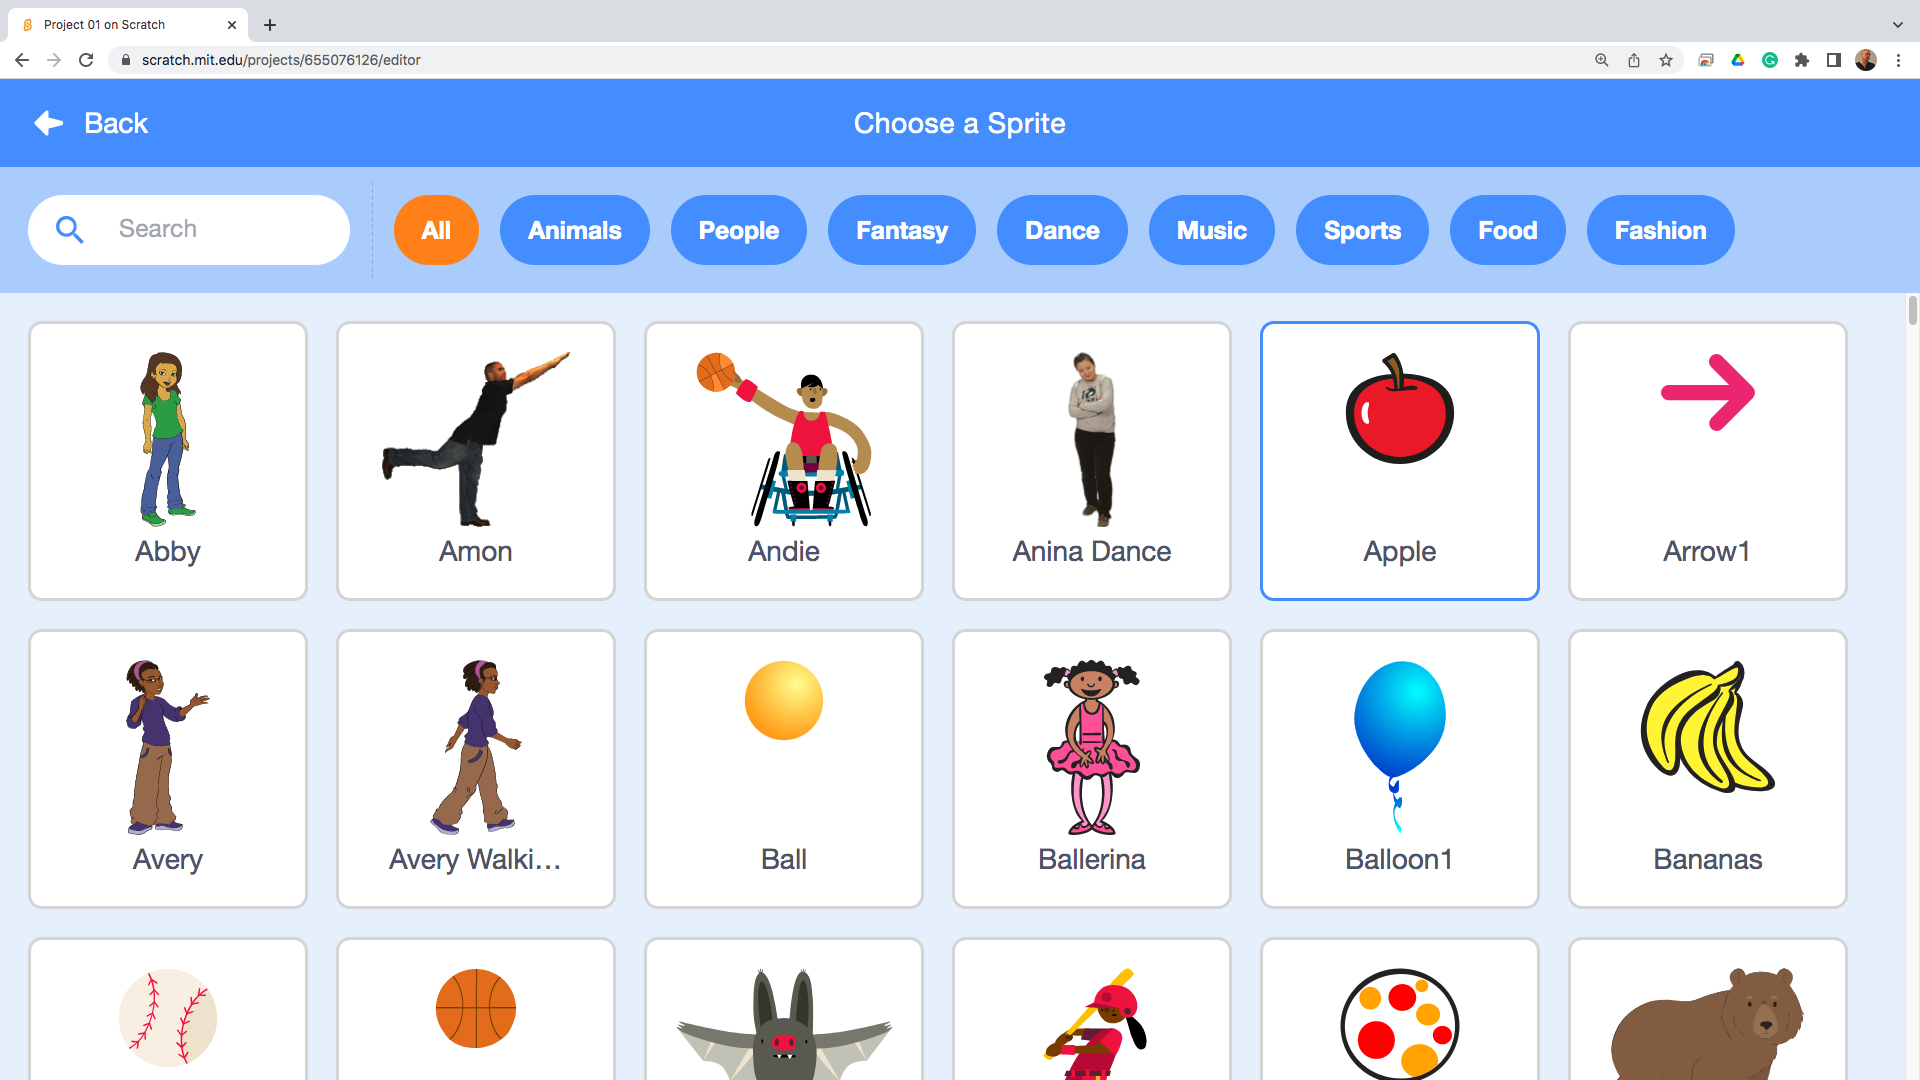
\includegraphics[width=1.0\linewidth,height=0.5\linewidth]{fig0093.png}
%  \caption{Избор на спрайт от галерията}
%\label{fig0093}
%\end{figure}
%
%\begin{figure}[H]
%  \centering
%  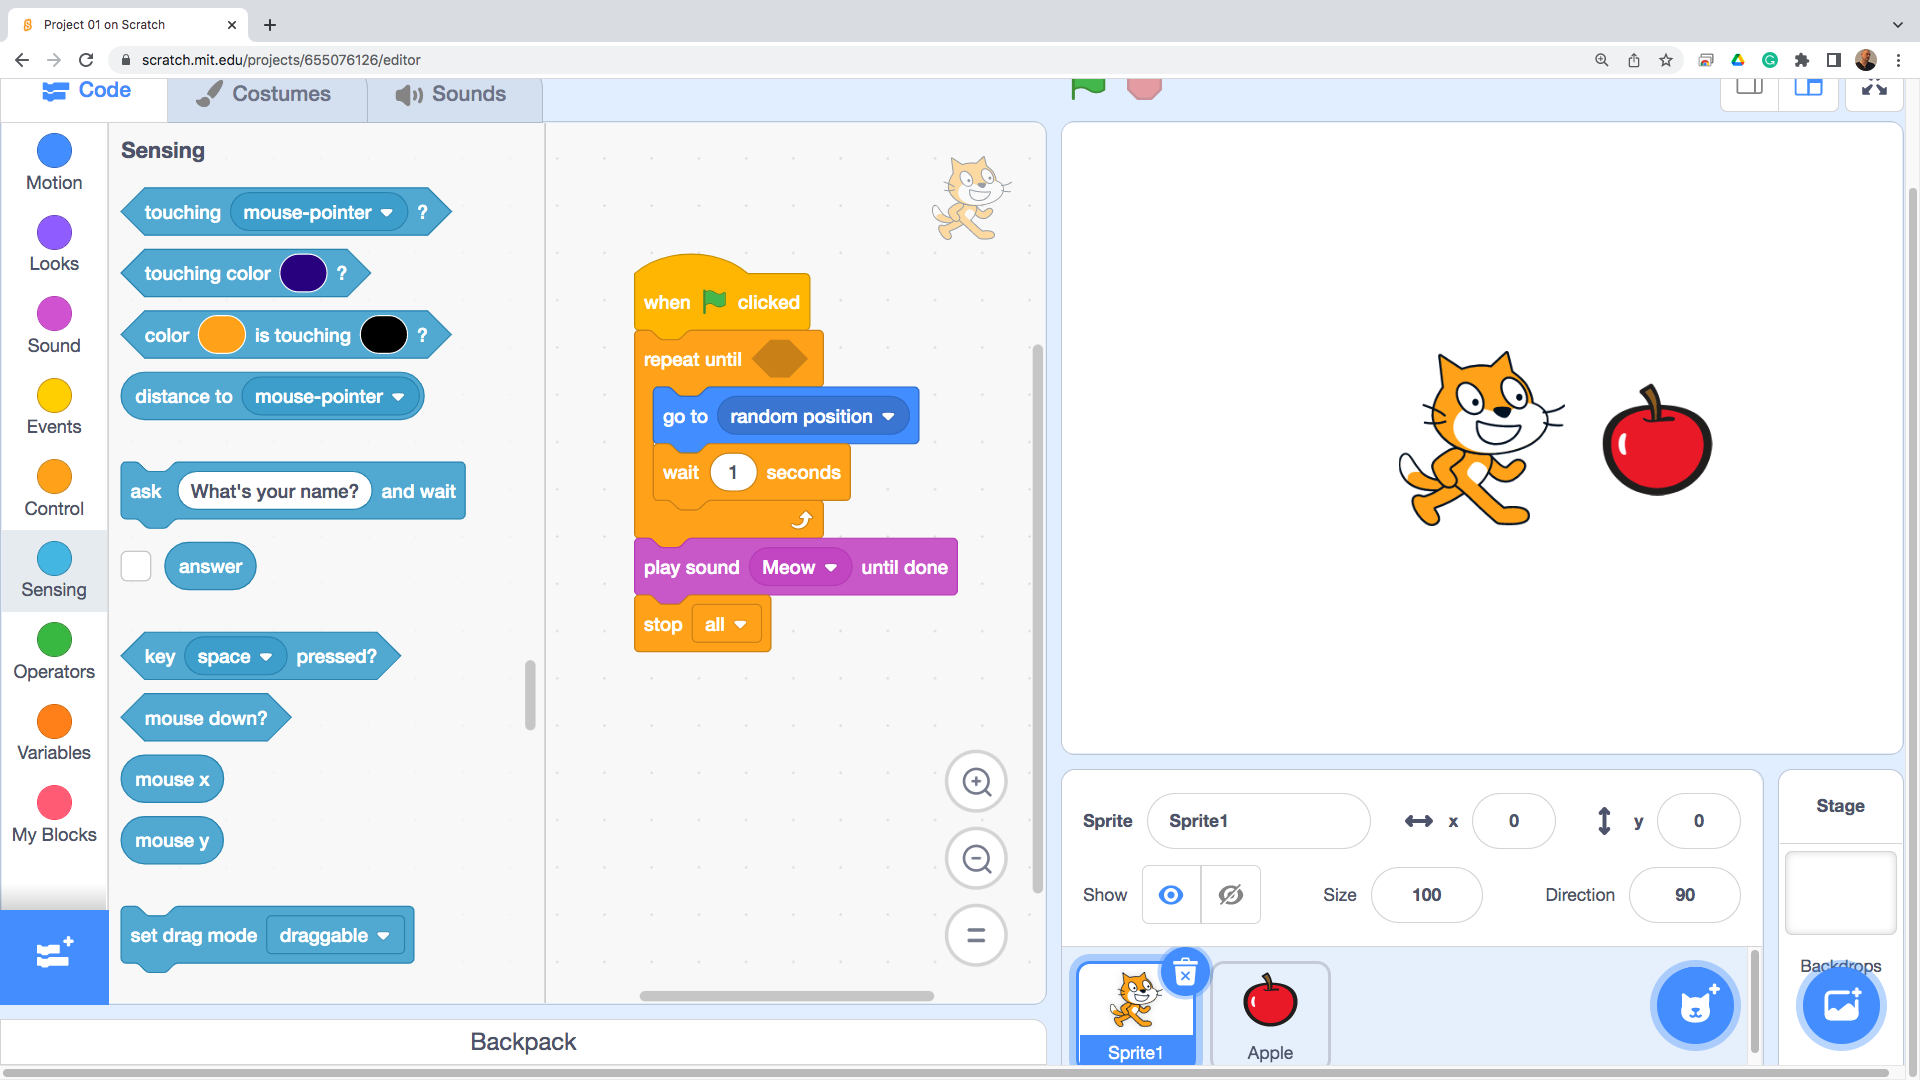
\includegraphics[width=1.0\linewidth,height=0.5\linewidth]{fig0094.png}
%  \caption{Позициониране на ябълката}
%\label{fig0094}
%\end{figure}
%
%При работата със спрайтове, една от най-често решаваните задачи е дали два спрайта се докосват или припокриват. Има различни техники за установяване на колизии между спрайтове, но една от най-ефективните е докосването на определен цвят. При съвременните компютри се работи с малко над 16 милиона различни цвята. Едно разумно подбиране на цветовете, които имат героите, може да даде безгранични възможности за откриване на колизии. Тъй като ябълката е червена, изборът за край на цикъла е когато котето докосне червения цвят (Фиг. \ref{fig0095}).
%
%\begin{figure}[H]
%  \centering
%  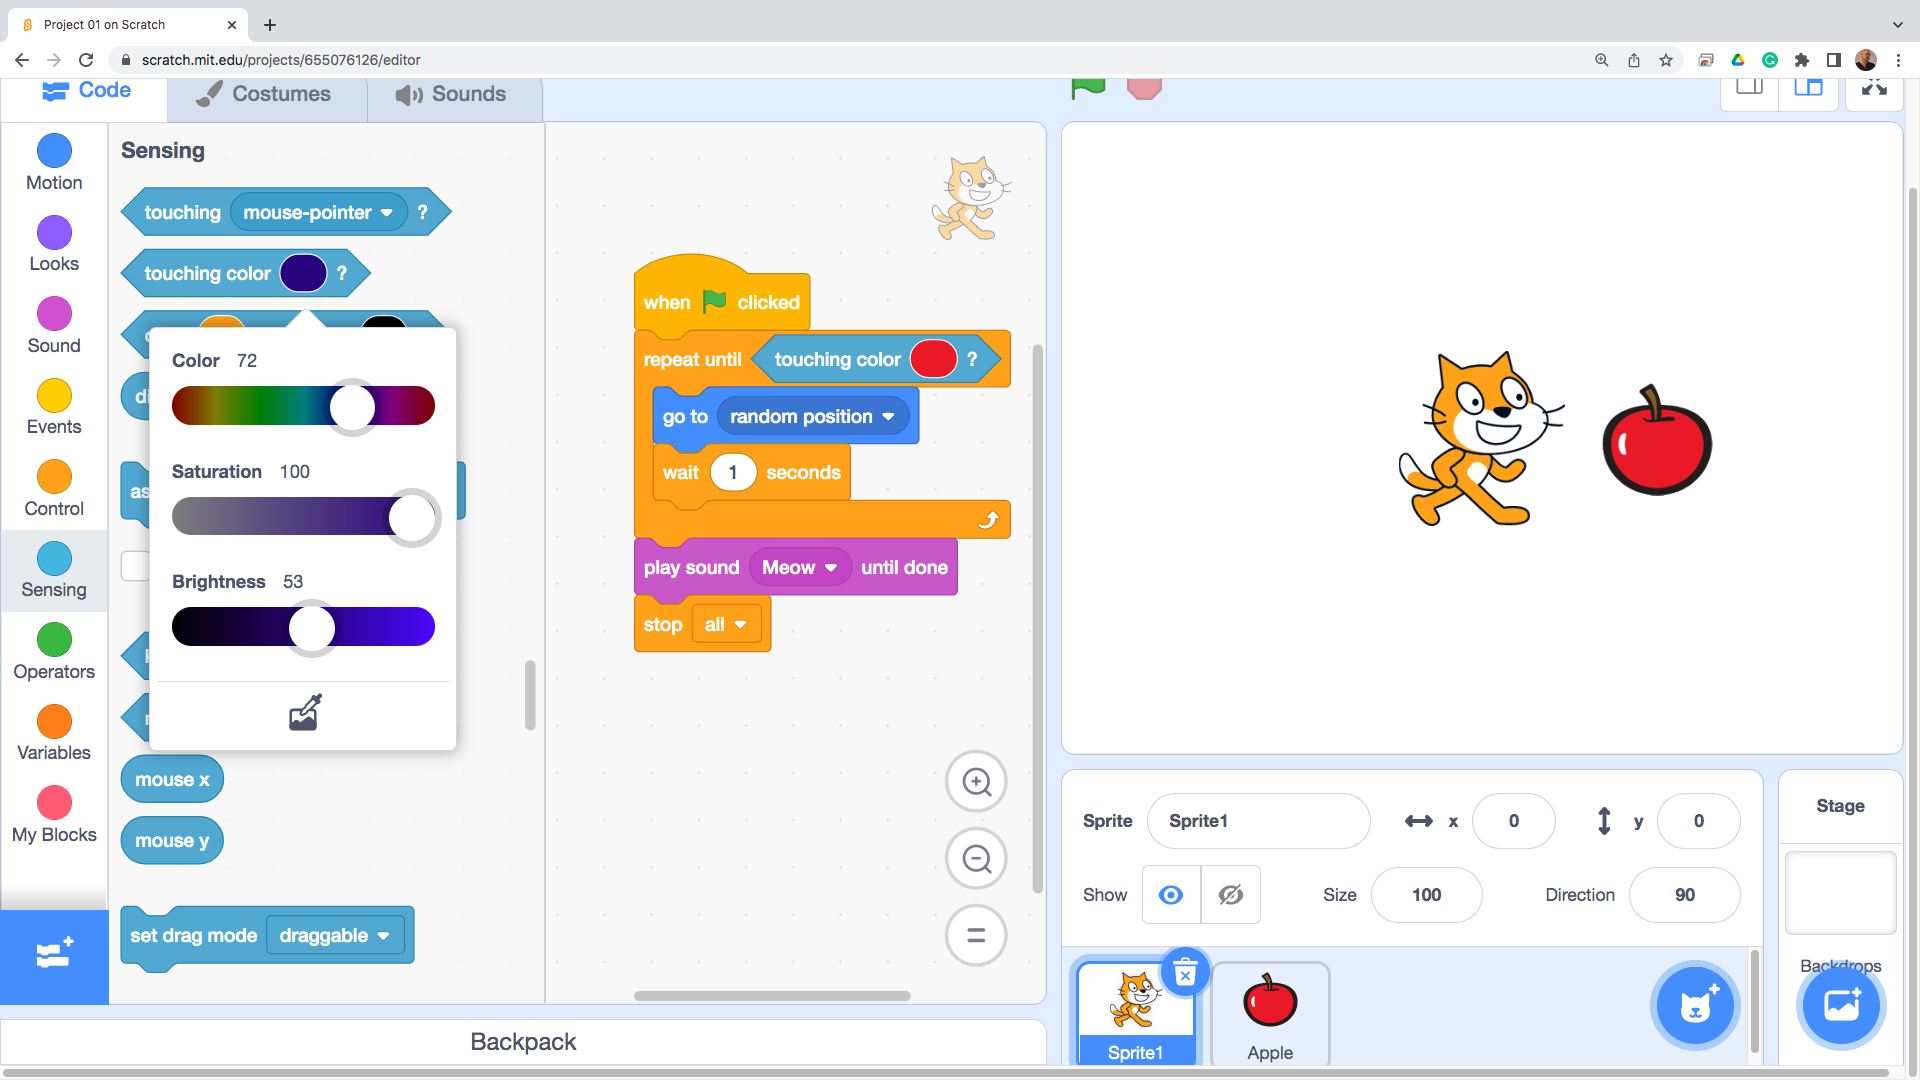
\includegraphics[width=1.0\linewidth,height=0.5\linewidth]{fig0095.png}
%  \caption{Докосване по цвят}
%\label{fig0095}
%\end{figure}
%
%С предходното блокче, независимо коя част на котето докосне ябълката, цикълът спира да се върти и се чува мяукането. Много по-фино определяне на колизията между спрайтовете може да се получи, ако само черният контур на котето се проверява за докосване до червения цвят на ябълката, за което служи следващото блокче (Фиг. \ref{fig0096}).
%
%\begin{figure}[H]
%  \centering
%  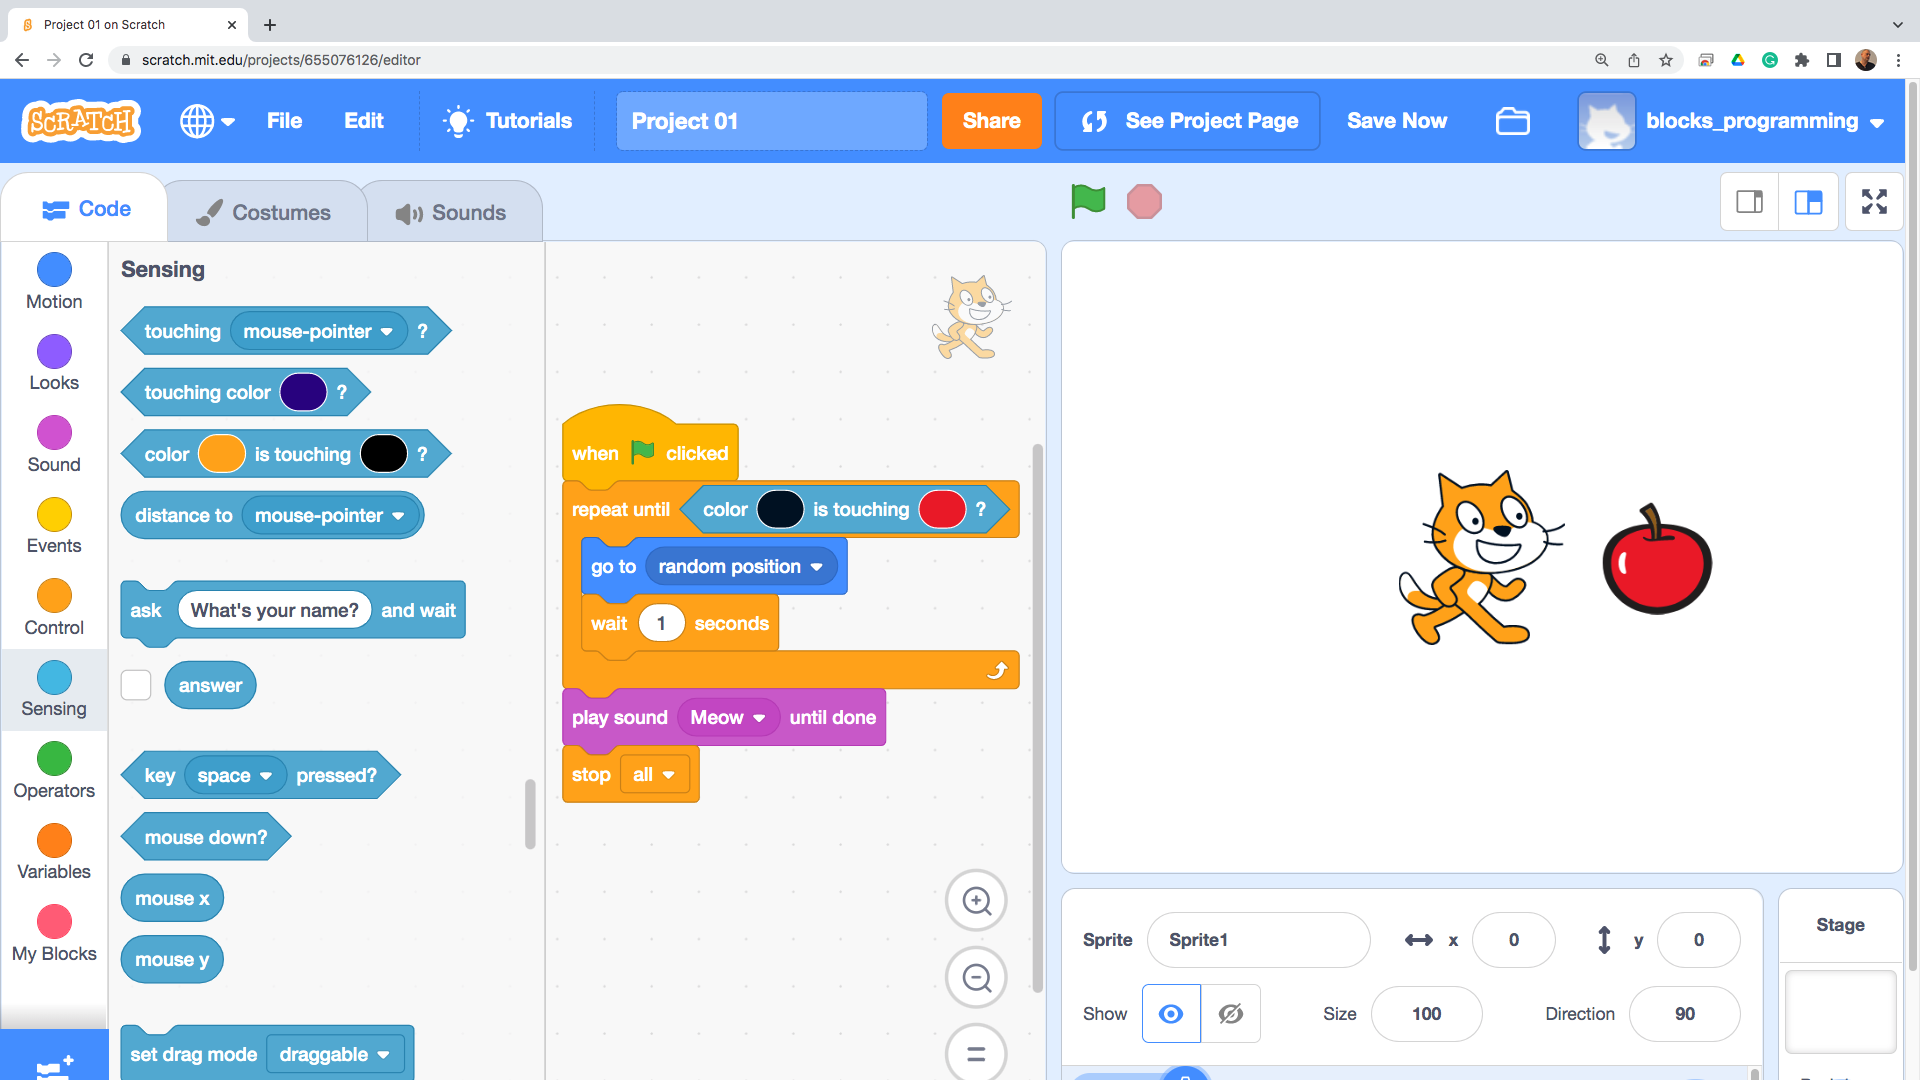
\includegraphics[width=1.0\linewidth,height=0.5\linewidth]{fig0096.png}
%  \caption{Колизия при два предварително зададени цвята}
%\label{fig0096}
%\end{figure}
%
%Следващото блокче е с овална форма и доставя на програмата разстоянието между спрайта и показалеца на мишката. Овалната форма подсказва, че това блокче трябва да бъде вградено в някое от блокчетата за аритметични изрази (Фиг. \ref{fig0097}).
%
%\begin{figure}[H]
%  \centering
%  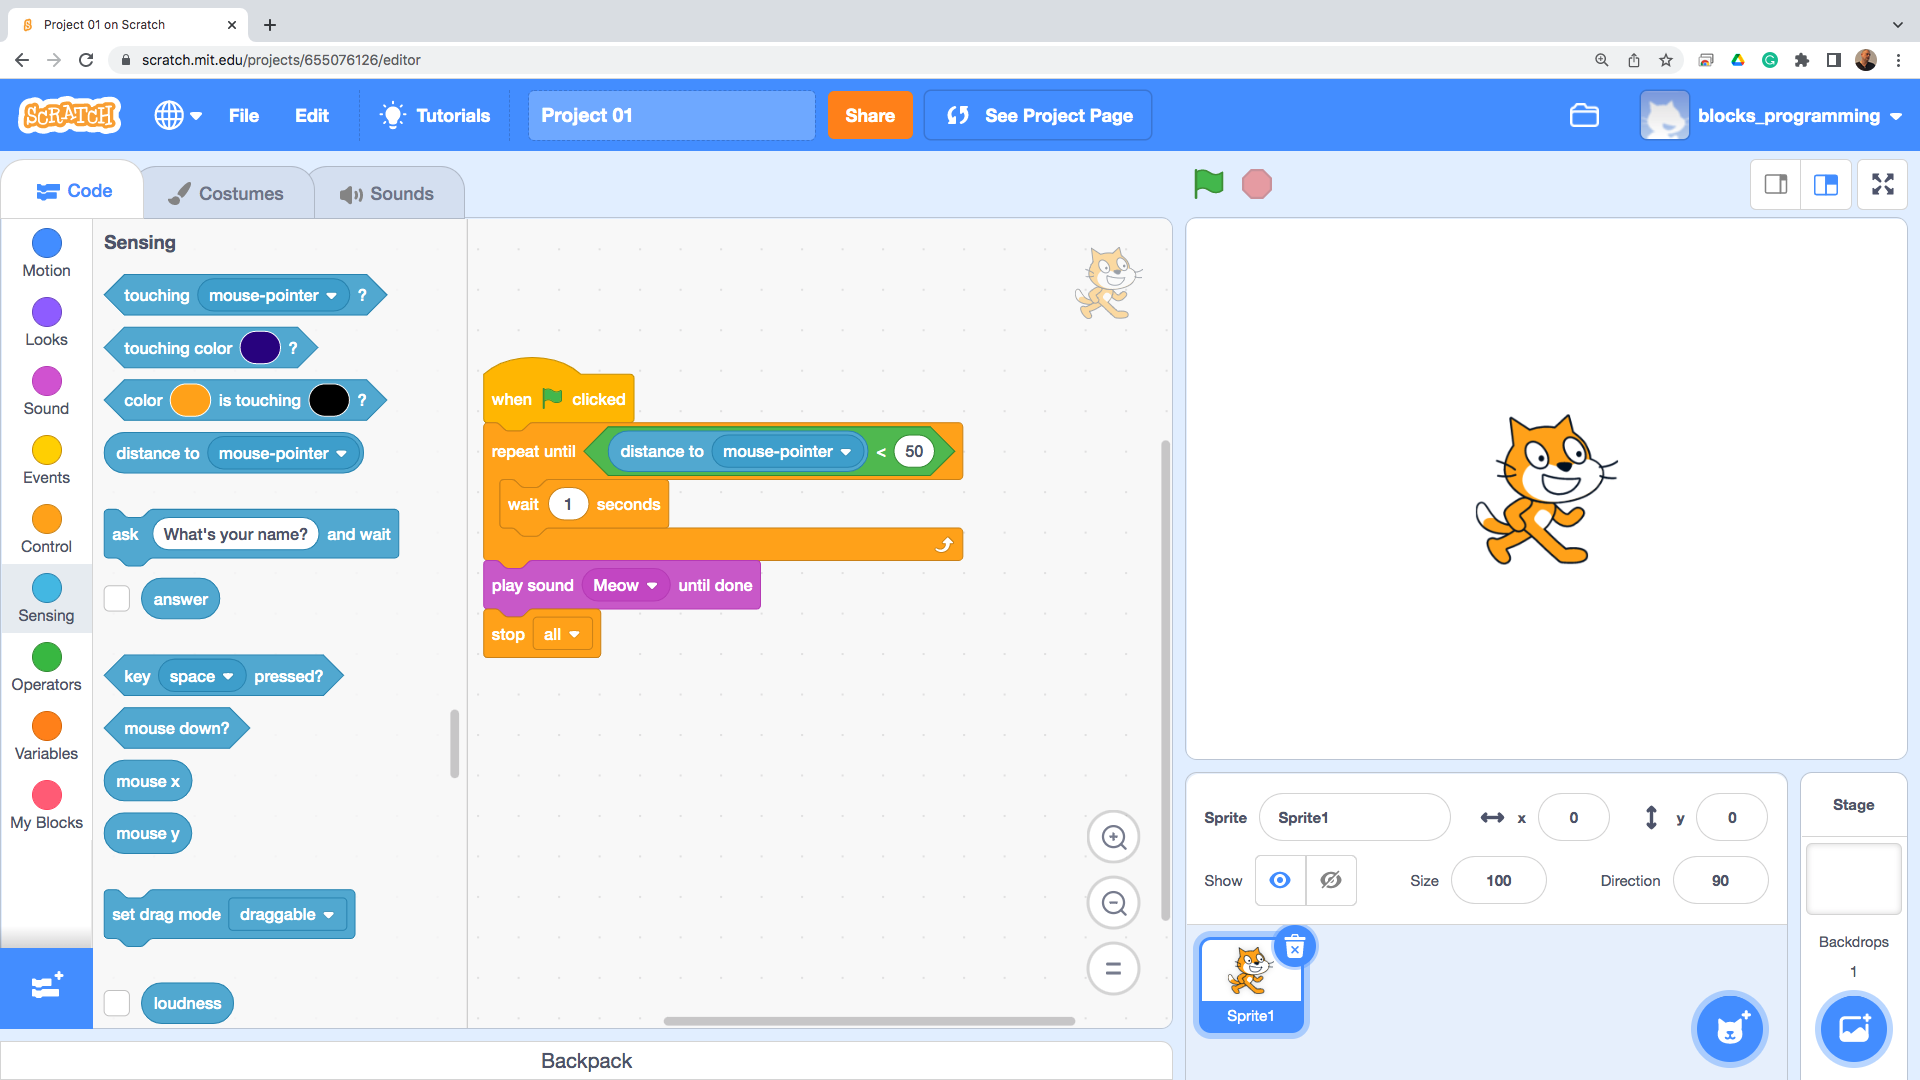
\includegraphics[width=1.0\linewidth,height=0.5\linewidth]{fig0097.png}
%  \caption{Разстояние до показалеца на мишката}
%\label{fig0097}
%\end{figure}
%
%Понякога се налага потребителят да напише нещо. За да се даде тази възможност е следващото блокче в групата на светло сините (Фиг. \ref{fig0098}). Анимираният герой подканя потребителя, като в конкретен текст подсказва какво се очаква да бъде написано. 
%
%\begin{figure}[H]
%  \centering
%  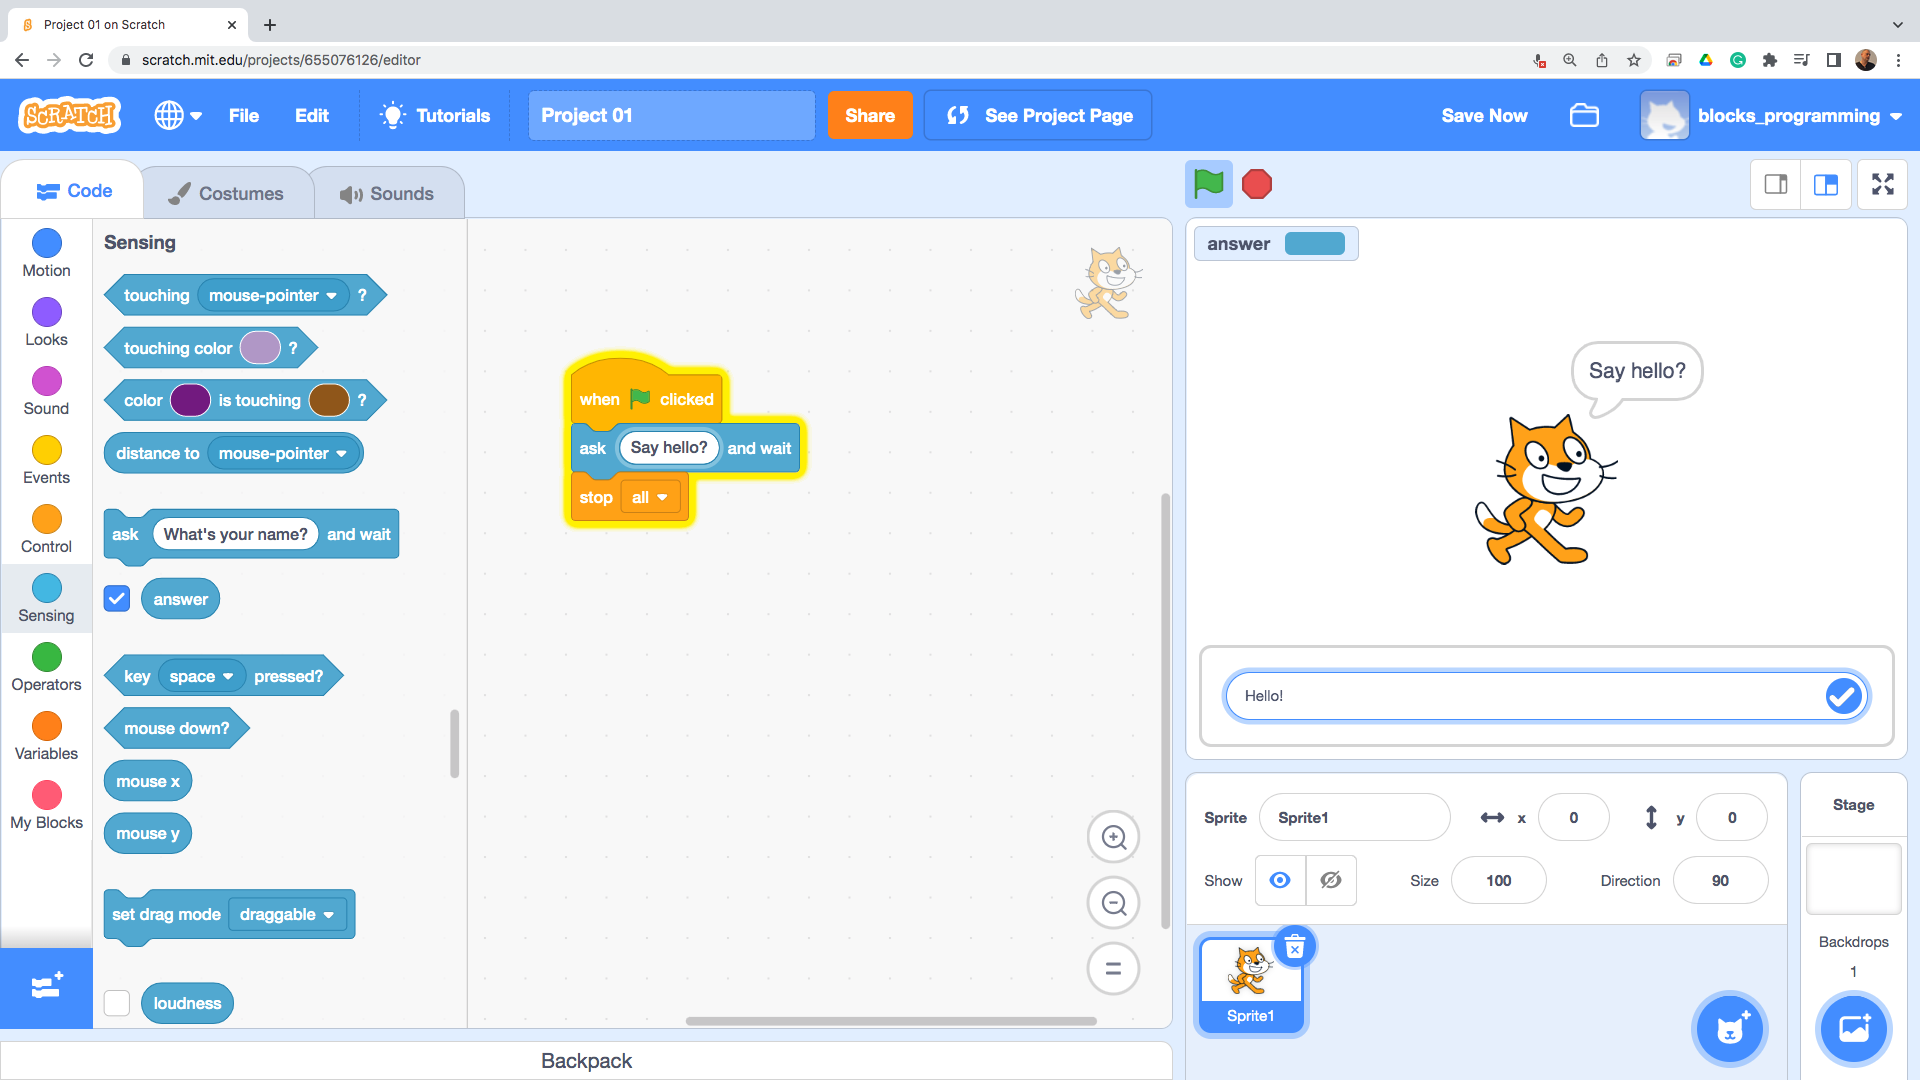
\includegraphics[width=1.0\linewidth,height=0.5\linewidth]{fig0098.png}
%  \caption{Въвеждане на текст}
%\label{fig0098}
%\end{figure}
%
%Следващото блокче е от шестоъгълните и е предназначено за вграждане. Това блокче връща резултат „истина“, когато бъде натиснат определен клавиш (Фиг. \ref{fig0099}).
%
%\begin{figure}[H]
%  \centering
%  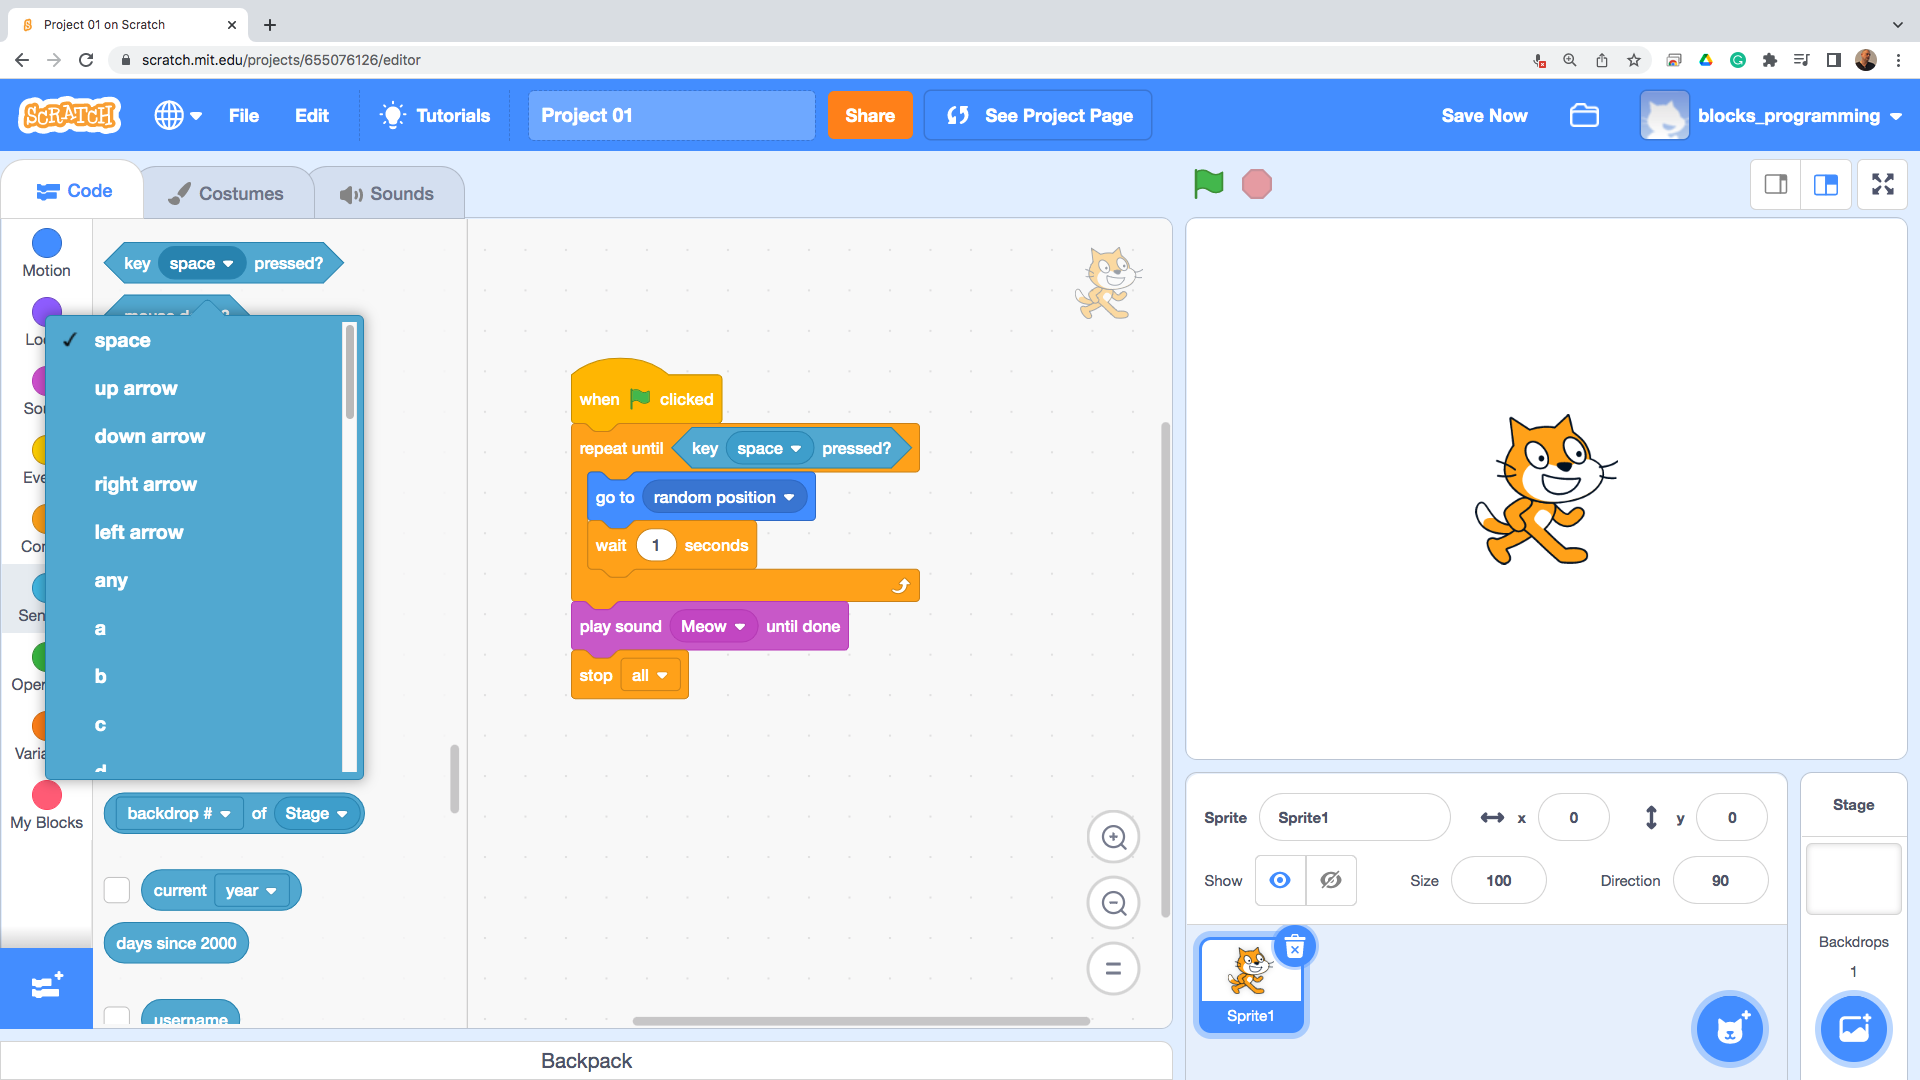
\includegraphics[width=1.0\linewidth,height=0.5\linewidth]{fig0099.png}
%  \caption{Определяне на натиснат клавиш}
%\label{fig0099}
%\end{figure}
%
%Сходно поведение може да се постигне и със следващото блокче, но вместо натискане на клавиш от клавиатурата се очаква натискане на клавиша на мишката (Фиг. \ref{fig0100}).
%
%\begin{figure}[H]
%  \centering
%  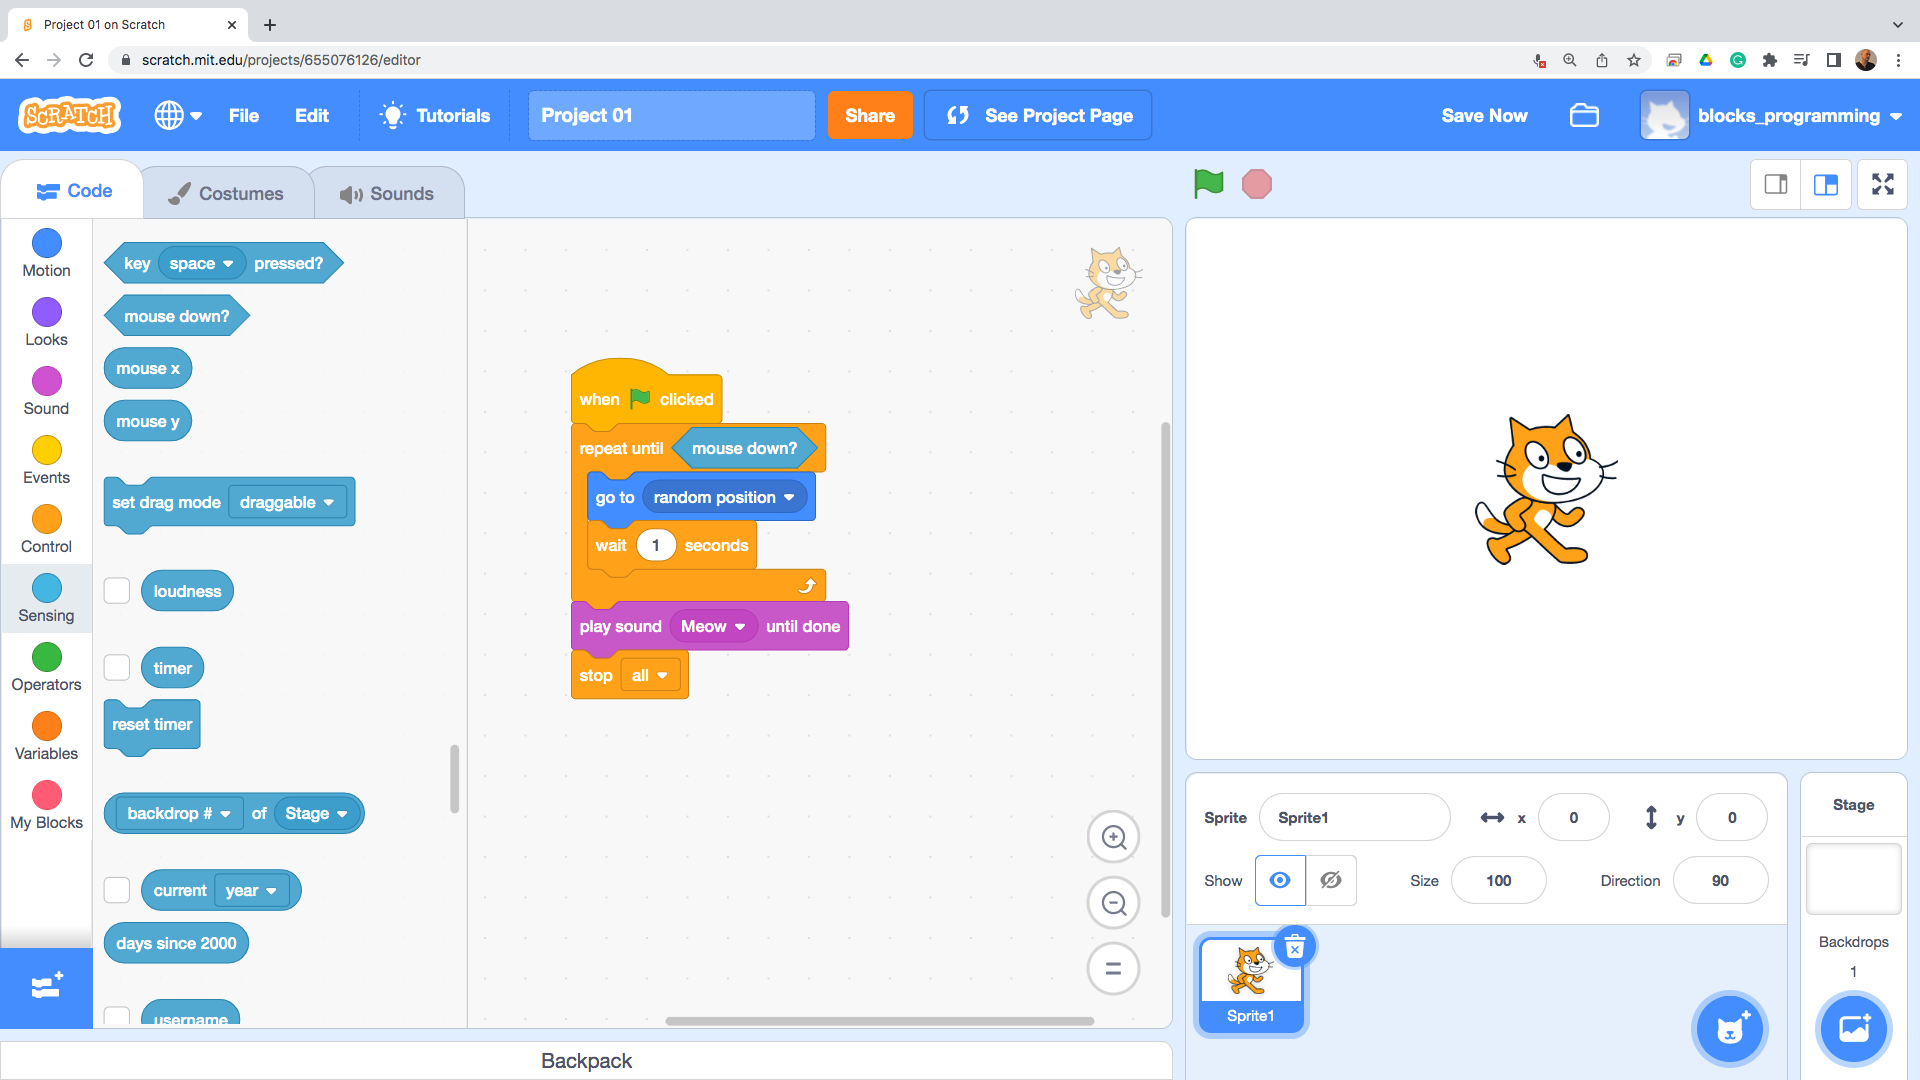
\includegraphics[width=1.0\linewidth,height=0.5\linewidth]{fig0100.png}
%  \caption{Определяне на натиснат бутон от мишката}
%\label{fig0100}
%\end{figure}
%
%Следващите две блокчета са овални и също са за вграждане. Първото дава координатите на анимирания герой по абцисната ос, а второто дава координатите на анимирания герой по ординатната ос (Фиг. \ref{fig0101}).
%
%\begin{figure}[H]
%  \centering
%  \includegraphics[width=1.0\linewidth,height=0.5\linewidth]{fig0101.png}
%  \caption{Координати на анимирания герой}
%\label{fig0101}
%\end{figure}
%
%По време на работа на програмата има функциониращ таймер, който отмерва времето от началото на изпълнението. Със следващото блокче този таймер може да се нулира (Фиг. \ref{fig0102}).
%
%\begin{figure}[H]
%  \centering
%  \includegraphics[width=1.0\linewidth,height=0.5\linewidth]{fig0102.png}
%  \caption{Нулиране на таймера}
%\label{fig0102}
%\end{figure}
%
%Следващото блокче е от овалните и служи за доставяне на информация за фона, променливи или нивото на звука (Фиг. \ref{fig0103}).
%
%\begin{figure}[H]
%  \centering
%  \includegraphics[width=1.0\linewidth,height=0.5\linewidth]{fig0103.png}
%  \caption{Информация за компоненти от сцената}
%\label{fig0103}
%\end{figure}
%
%Последното блокче в групата е предвидено също за вграждане и връща броя дни от година 2000 (Фиг. \ref{fig0104}).
%
%\begin{figure}[H]
%  \centering
%  \includegraphics[width=1.0\linewidth,height=0.5\linewidth]{fig0104.png}
%  \caption{Брой дни от началото на века}
%\label{fig0104}
%\end{figure}
%
%Групата на зелените блокчета е предназначена за вграждане. Първите четири блокчета са с овална форма и са предвидени за аритметичните операции – събиране, изваждане, умножение и делене (Фиг. \ref{fig0105}).
%
%\begin{figure}[H]
%  \centering
%  \includegraphics[width=1.0\linewidth,height=0.5\linewidth]{fig0105.png}
%  \caption{Аритметични операции}
%\label{fig0105}
%\end{figure}
%
%Блокчето за избор на случайно число вече е демонстрирано, но то идеално пасва в трите блокчета, които следват след него. Това са блокчета за сравнение и са предвидени за вграждане в блокчетата за управление на изпълнението (Фиг. \ref{fig0106}).
%
%\begin{figure}[H]
%  \centering
%  \includegraphics[width=1.0\linewidth,height=0.5\linewidth]{fig0106.png}
%  \caption{Операции за сравнение}
%\label{fig0106}
%\end{figure}
%
%Следват три блокчета с шестоъгълна форма (Фиг. \ref{fig0107}), които служат за вграждане в блокчета за контрол на управлението. Трите блокчета изпълняват трите основни логически операции („и“, „или“, „не“). При първото блокче и двете условия трябва да са изпълнени за да се влезе в конструкцията за условен преход. Точно поради тази причина, логическата операция се нарича „и“. При второто блокче или едното условие, или другото условие трябва да бъде изпълнено, за да се влезе в конструкцията за условен преход. Точно поради тази причина, логическата операция се нарича „или“. При третото блокче, резултата се обръща, така че в конструкцията за условен преход се влиза при невярно условие. Поради тази причина, тази операция се нарича „отрицание“.
%
%\begin{figure}[H]
%  \centering
%  \includegraphics[width=1.0\linewidth,height=0.5\linewidth]{fig0107.png}
%  \caption{Логически операции}
%\label{fig0107}
%\end{figure}
%
%Следващите четири блокчета са за работа със символни низове (Фиг. \ref{fig0108}). Първите три са с овална форма, а последното е с шестоъгълна форма. Първото блокче слепва два символни низа. Второто блокче определя буква на определена позиция в символния низ. Третото блокче определя дължината на символния низ. Четвъртото блокче търси определена буква в символния низ. 
%
%\begin{figure}[H]
%  \centering
%  \includegraphics[width=1.0\linewidth,height=0.5\linewidth]{fig0108.png}
%  \caption{Работа със символни низове}
%\label{fig0108}
%\end{figure}
%
%Последните три блокчета в групата на зелените са предназначени за работа с функции (Фиг. \ref{fig0109}). Първото блокче изчислява остатъкът от целочислено делене. Второто блокче закръглява дробно число до цялата му част. Третото блокче предлага пресмятането на цял списък от математически функции. 
%
%\begin{figure}[H]
%  \centering
%  \includegraphics[width=1.0\linewidth,height=0.5\linewidth]{fig0109.png}
%  \caption{Математически функции}
%\label{fig0109}
%\end{figure}
%
%Последната група блокчета е групата на тъмно оранжевите (Фиг. \ref{fig0110}). Те са предназначени за работа с променливи. Често при писането на програми е необходимо междинните пресметнати резултати да бъдат запазени временно и в последствие да бъдат използвани за следващи пресмятания. Това се постига чрез променливите. Променливите са временни контейнери, които съхраняват зададените им стойности. Първото блокче в групата служи за установяване на стойност на променливата. Второто блокче в групата служи за промяна на стойността на променливата. Третото блокче в групата служи за програмна визуализация на променливата. Последното блокче в групата служи за скриване на визуализацията. 
%
%\begin{figure}[H]
%  \centering
%  \includegraphics[width=1.0\linewidth,height=0.5\linewidth]{fig0110.png}
%  \caption{Работа с променливи}
%\label{fig0110}
%\end{figure}
%
%След като вече са представени всички най-важни конструкции в програмната среда на Scratch, може да се премине към следващите стъпки за писането на по-сложни програми, съчетавайки базовите блокчета по подходящ начин.

\section{Изразни средства в App Inventor}

Основна разлика между App Inventor и Scratch е, че в App Inventor не се използват спрайтове, а се изгражда графичен потребителски интерфейс. Причината за това е, че App Inventor стъпва на класическия подход за писане на Android приложения. Тази разлика налага да се разгледат два вида изразни средства в App Inventor, а именно компонентите на графичния интерфейс и програмните блокчета за изграждане на серия от инструкции.

Изграждането на приложение в App Inventor започва в нов, празен екран (Фиг. \ref{fig0111}). Екраните се наричат сцени и работата на програмата преминава от сцена в сцена. Когато програмата е нещо съвсем простичка, може да се реализира и само е една сцена. 

\begin{figure}[H]
  \centering
  \includegraphics[width=1.0\linewidth,height=0.5\linewidth]{fig0111.png}
  \caption{Начална сцена}
\label{fig0111}
\end{figure}

\subsection{Графичен интерфейс}

Компонентите на графичния интерфейс са организирани в групи, както са организирани блокчетата за изпълнение на инструкции. Повечето визуални компоненти имат графично оформление, директно на екрана, но има и компоненти, които не се визуализират. Пример за не визуализиращи се компоненти са мениджърите за управление на оформлението. Тези мениджъри са представени във втората група и функцията им е да служат като групиращи компоненти, които подреждат визуално представените компоненти. 

От дясно на работната сцена е представена йерархична структура на позиционираните графични компоненти. В този панел може да се изтриват компоненти или да бъдат преименувани. Най- в дясно е разположен панел с характеристиките на текущо избрания графичен компоненти. Компонентите имат различни характеристики и те могат да се установяват докато се проектира самия интерфейс. 

В първата група са включени основните компоненти за изграждане на графичен потребителски интерфейс. Първият компонент в тази група е бутонът (Фиг. \ref{fig0112}). Поставянето му в работната площ на сцената става чрез избиране с мишката и влачене до работното пространство. Бутонът има характеристики свързани с текста върху самия компонент, възможността за поставяне на изображение, размери, форма, големина на шрифта, цветове на фона и на предния план, както и някои други.

\begin{figure}[H]
  \centering
  \includegraphics[width=1.0\linewidth,height=0.5\linewidth]{fig0112.png}
  \caption{Графичен компонент за бутон}
\label{fig0112}
\end{figure}

След бутона следва компонент за маркиране (Фиг. \ref{fig0113}), който има сходна функционалност на бутона, но се маркира състояние на включен или изключен. Често намира приложение за обозначаване на свойства. Най-важната характеристика на този компонент е дали е в установено състояние или в изключено. 

\begin{figure}[H]
  \centering
  \includegraphics[width=1.0\linewidth,height=0.5\linewidth]{fig0113.png}
  \caption{Графичен компонент за отмятане}
\label{fig0113}
\end{figure}

Въвеждането на дати от потребителя е процес, който може да доведе до много грешки. Причината за това е, че различните месеци имат различна продължителност, а месец февруари се определя от високосните години и дали съответната високосна година е кратна на четиристотин. За да се избегнат грешките при въвеждането на дати Android предлага визуален компонент, който да се ползва за контролирано въвеждане на дати (Фиг. \ref{fig0114}).

\begin{figure}[H]
  \centering
  \includegraphics[width=1.0\linewidth,height=0.5\linewidth]{fig0114.png}
  \caption{Графичен компонент за въвеждане на дати}
\label{fig0114}
\end{figure}

При различните версии или частни модификации на операционната система Android, компонентът за въвеждане на дати може да има различно представяне. Една от възможностите е под формата на брояч с три сегмента за ден, месец и година (Фиг. \ref{fig0115}).

\begin{figure}[H]
  \centering
  \includegraphics[width=1.0\linewidth,height=0.5\linewidth]{fig0115.png}
  \caption{Въвеждане на дата}
\label{fig0115}
\end{figure}

\subsection{Програмни конструкции}

